%%%%%%%%%%%%%%%%%%%%%%%%%%%%%%%%%%%%%%%%%
% Classicthesis Typographic Thesis
% LaTeX Template
% Version 1.3 (15/2/14)
%
% This template has been downloaded from:
% http://www.LaTeXTemplates.com
%
% Original author:
% André Miede (http://www.miede.de)
%
% License:
% CC BY-NC-SA 3.0 (http://creativecommons.org/licenses/by-nc-sa/3.0/)
%
% General Tips:
% 1) Make sure to edit the classicthesis-config.file
% 2) New enumeration (A., B., C., etc in small caps): \begin{aenumerate} \end{aenumerate}
% 3) For margin notes: \marginpar or \graffito{}
% 4) Do not use bold fonts in this style, it is designed around them
% 5) Use tables as in the examples
% 6) See classicthesis-preamble.sty for useful commands
%
%%%%%%%%%%%%%%%%%%%%%%%%%%%%%%%%%%%%%%%%%

%----------------------------------------------------------------------------------------
%	PACKAGES AND OTHER DOCUMENT CONFIGURATIONS
%----------------------------------------------------------------------------------------

\documentclass[
		twoside,openright,titlepage,numbers=noenddot,headinclude,%1headlines,
                footinclude=true,cleardoublepage=empty,
                BCOR=5mm,paper=a4,fontsize=11pt, % Binding correction, paper type and font size
                ngerman,american, % Languages
                ]{scrreprt} 
                
% Includes the file which contains all the document configurations and packages - make sure to edit this file
%%%%%%%%%%%%%%%%%%%%%%%%%%%%%%%%%%%%%%%%%
% Thesis Configuration File
%
% The main lines to change in this file are in the DOCUMENT VARIABLES
% section, the rest of the file is for advanced configuration.
%
%%%%%%%%%%%%%%%%%%%%%%%%%%%%%%%%%%%%%%%%%

%----------------------------------------------------------------------------------------
%	DOCUMENT VARIABLES
%	Fill in the lines below to enter your information into the thesis template
%	Each of the commands can be cited anywhere in the thesis
%----------------------------------------------------------------------------------------

% Remove drafting to get rid of the '[ Date - classicthesis version 4.0 ]' text at the bottom of every page
\PassOptionsToPackage{eulerchapternumbers,listings,pdfspacing,subfig,beramono,parts,manychapters}{classicthesis}
% Available options: drafting parts nochapters linedheaders eulerchapternumbers beramono eulermath pdfspacing minionprospacing tocaligned dottedtoc manychapters listings floatperchapter subfig
% Adding 'dottedtoc' will make page numbers in the table of contents flushed right with dots leading to them

\newcommand{\myTitle}{Computer-Assisted Translation at the Service of Translators\xspace}
\newcommand{\mySubtitle}{A Unified Methodology\xspace}
\newcommand{\myDegree}{Master's Programme in Language Technology\xspace}
\newcommand{\myName}{Daniel Vidal Hussey\xspace}
\newcommand{\myProf}{Put name here\xspace}
\newcommand{\myOtherProf}{Put name here\xspace}
\newcommand{\mySupervisor}{Aarne Ranta\xspace}
\newcommand{\myExaminer}{Simon Dobnik}
\newcommand{\myFaculty}{Faculty of Arts\xspace}
\newcommand{\myDepartment}{Department of Philosophy, Linguistics and Theory of Science\xspace}
\newcommand{\myUni}{University of Gothenburg\xspace}
\newcommand{\myLocation}{Gothenburg, Sweden\xspace}
\newcommand{\myTime}{September 2015\xspace}
\newcommand{\myVersion}{Version 1.0\xspace}

%----------------------------------------------------------------------------------------
%	USEFUL COMMANDS
%----------------------------------------------------------------------------------------

\newcommand{\ie}{i.\,e.\xspace}
\newcommand{\Ie}{I.\,e.\xspace}
\newcommand{\eg}{e.\,g.\xspace}
\newcommand{\Eg}{E.\,g.\xspace} 

\newcommand{\style}{\spacedlowsmallcaps{style}\xspace} 
\newcommand{\scratch}{\spacedlowsmallcaps{scratch}\xspace} 
\newcommand{\charlotte}{\spacedlowsmallcaps{charlotte}\xspace}
\newcommand{\ai}{\spacedlowsmallcaps{ai}\xspace}
\newcommand{\garfield}{\spacedlowsmallcaps{garfield}\xspace}

\newcounter{dummy} % Necessary for correct hyperlinks (to index, bib, etc.)
\providecommand{\mLyX}{L\kern-.1667em\lower.25em\hbox{Y}\kern-.125emX\@}

%----------------------------------------------------------------------------------------
%	PACKAGES
%----------------------------------------------------------------------------------------

\usepackage{minted}
%\usemintedstyle{manni}
%\usepackage{scrhack}

%------------------------------------------------

%\usepackage{lipsum} % Used for inserting dummy 'Lorem ipsum' text into the template
%------------------------------------------------
 
%\PassOptionsToPackage{latin9}{inputenc} % latin9 (ISO-8859-9) = latin1+"Euro sign"
\PassOptionsToPackage{utf8}{inputenc} % UTF-8
\usepackage{inputenc}
 
 %------------------------------------------------

%\PassOptionsToPackage{ngerman,american}{babel}  % Change this to your language(s)
%\PassOptionsToPackage{american}{babel}  % Change this to your language(s)
% Spanish languages need extra options in order to work with this template
\PassOptionsToPackage{spanish,es-lcroman}{babel}
\usepackage{babel}

%------------------------------------------------			

%\PassOptionsToPackage{square,numbers}{natbib}
%\PassOptionsToPackage{authoryear,round,colon}{natbib}
% \usepackage{natbib}
 % Use (author, year) style http://tex.stackexchange.com/questions/130858/classicthesis-citation-style-author-year-instead-of-numerical
\usepackage[
    backend=biber,
    style=authoryear,
    sorting=nyt,
    citestyle=apa,
    backref=true
]{biblatex}
 \addbibresource{Bibliography.bib}
 \DefineBibliographyStrings{english}{%
  backrefpage = {Cited on page},% originally "cited on page"
  backrefpages = {Cited on pages},% originally "cited on pages"
}
 
 %------------------------------------------------

\PassOptionsToPackage{fleqn}{amsmath} % Math environments and more by the AMS 
 \usepackage{amsmath}
 
 %------------------------------------------------

\PassOptionsToPackage{T1}{fontenc} % T2A for cyrillics
\usepackage{fontenc}

%------------------------------------------------

\usepackage{xspace} % To get the spacing after macros right

%------------------------------------------------

\usepackage{mparhack} % To get marginpar right

%------------------------------------------------

%\usepackage{fixltx2e} % Fixes some LaTeX stuff 

%------------------------------------------------

\PassOptionsToPackage{smaller}{acronym} % Include printonlyused in the first bracket to only show acronyms used in the text
\usepackage{acronym} % nice macros for handling all acronyms in the thesis

%------------------------------------------------

%\renewcommand*{\acsfont}[1]{\textssc{#1}} % For MinionPro
%\renewcommand{\bflabel}[1]{{#1}\hfill} % Fix the list of acronyms

%------------------------------------------------

\PassOptionsToPackage{pdftex}{graphicx}
\usepackage{graphicx} 

%----------------------------------------------------------------------------------------
%	FLOATS: TABLES, FIGURES AND CAPTIONS SETUP
%----------------------------------------------------------------------------------------

\usepackage{tabularx} % Better tables
\setlength{\extrarowheight}{3pt} % Increase table row height
\newcommand{\tableheadline}[1]{\multicolumn{1}{c}{\spacedlowsmallcaps{#1}}}
\newcommand{\myfloatalign}{\centering} % To be used with each float for alignment
\usepackage{caption}
\captionsetup{format=hang,font=small}
\usepackage{subfig}  

%----------------------------------------------------------------------------------------
%	CODE LISTINGS SETUP
%----------------------------------------------------------------------------------------

\usepackage{listings} 
%\lstset{emph={trueIndex,root},emphstyle=\color{BlueViolet}}%\underbar} % for special keywords
\lstset{language=[LaTeX]Tex, % Specify the language for listings here
keywordstyle=\color{RoyalBlue}, % Add \bfseries for bold
basicstyle=\small\ttfamily, % Makes listings a smaller font size and a different font
%identifierstyle=\color{NavyBlue}, % Color of text inside brackets
commentstyle=\color{Green}\ttfamily, % Color of comments
stringstyle=\rmfamily, % Font type to use for strings
numbers=left, % Change left to none to remove line numbers
numberstyle=\scriptsize, % Font size of the line numbers
stepnumber=1, % Increment of line numbers
numbersep=8pt, % Distance of line numbers from code listing
showstringspaces=false, % Sets whether spaces in strings should appear underlined
breaklines=true, % Force the code to stay in the confines of the listing box
%frameround=ftff, % Uncomment for rounded frame
frame=tb, % Frame border - none/leftline/topline/bottomline/lines/single/shadowbox/L
belowcaptionskip=.75\baselineskip % Space after the "Listing #: Desciption" text and the listing box
}

%----------------------------------------------------------------------------------------
%	HYPERREFERENCES
%----------------------------------------------------------------------------------------

\PassOptionsToPackage{pdftex,hyperfootnotes=false,pdfpagelabels}{hyperref}
\usepackage{hyperref}  % backref linktocpage pagebackref
\pdfcompresslevel=9
\pdfadjustspacing=1

\hypersetup{
% Uncomment the line below to remove all links (to references, figures, tables, etc)
%draft, 
colorlinks=true, linktocpage=true, pdfstartpage=3, pdfstartview=FitV,
% Uncomment the line below if you want to have black links (e.g. for printing black and white)
%colorlinks=false, linktocpage=false, pdfborder={0 0 0}, pdfstartpage=3, pdfstartview=FitV, 
breaklinks=true, pdfpagemode=UseNone, pageanchor=true, pdfpagemode=UseOutlines,
plainpages=false, bookmarksnumbered, bookmarksopen=true, bookmarksopenlevel=1,
hypertexnames=true, pdfhighlight=/O, urlcolor=webbrown, linkcolor=RoyalBlue, citecolor=webgreen,
%------------------------------------------------
% PDF file meta-information
pdftitle={\myTitle},
pdfauthor={\textcopyright\ \myName, \myUni, \myDepartment},
pdfsubject={},
pdfkeywords={},
pdfcreator={pdfLaTeX},
pdfproducer={LaTeX with hyperref and classicthesis}
%------------------------------------------------
}   

%----------------------------------------------------------------------------------------
%	BACKREFERENCES
%----------------------------------------------------------------------------------------

\usepackage{ifthen} % Allows the user of the \ifthenelse command
\newboolean{enable-backrefs} % Variable to enable backrefs in the bibliography
\setboolean{enable-backrefs}{false} % Variable value: true or false

\newcommand{\backrefnotcitedstring}{\relax} % (Not cited.)
\newcommand{\backrefcitedsinglestring}[1]{(Cited on page~#1.)}
\newcommand{\backrefcitedmultistring}[1]{(Cited on pages~#1.)}
\ifthenelse{\boolean{enable-backrefs}} % If backrefs were enabled
{
\PassOptionsToPackage{hyperpageref}{backref}
\usepackage{backref} % to be loaded after hyperref package 
\renewcommand{\backreftwosep}{ and~} % separate 2 pages
\renewcommand{\backreflastsep}{, and~} % separate last of longer list
\renewcommand*{\backref}[1]{}  % disable standard
\renewcommand*{\backrefalt}[4]{% detailed backref
\ifcase #1 
\backrefnotcitedstring
\or
\backrefcitedsinglestring{#2}
\else
\backrefcitedmultistring{#2}
\fi}
}{\relax} 

%----------------------------------------------------------------------------------------
%	AUTOREFERENCES SETUP
%	Redefines how references in text are prefaced for different 
%	languages (e.g. "Section 1.2" or "section 1.2")
%----------------------------------------------------------------------------------------

\makeatletter
\@ifpackageloaded{babel}
{
\addto\extrasamerican{
\renewcommand*{\figureautorefname}{Figure}
\renewcommand*{\tableautorefname}{Table}
\renewcommand*{\partautorefname}{Part}
\renewcommand*{\chapterautorefname}{Chapter}
\renewcommand*{\sectionautorefname}{Section}
\renewcommand*{\subsectionautorefname}{Section}
\renewcommand*{\subsubsectionautorefname}{Section}
}
\addto\extrasngerman{
\renewcommand*{\paragraphautorefname}{Absatz}
\renewcommand*{\subparagraphautorefname}{Unterabsatz}
\renewcommand*{\footnoteautorefname}{Fu\"snote}
\renewcommand*{\FancyVerbLineautorefname}{Zeile}
\renewcommand*{\theoremautorefname}{Theorem}
\renewcommand*{\appendixautorefname}{Anhang}
\renewcommand*{\equationautorefname}{Gleichung}
\renewcommand*{\itemautorefname}{Punkt}
}
\providecommand{\subfigureautorefname}{\figureautorefname} % Fix to getting autorefs for subfigures right
}{\relax}
\makeatother

%----------------------------------------------------------------------------------------
\usepackage{classicthesis} 
%----------------------------------------------------------------------------------------
%	CHANGING TEXT AREA 
%----------------------------------------------------------------------------------------

%\linespread{1.05} % a bit more for Palatino
%\areaset[current]{312pt}{761pt} % 686 (factor 2.2) + 33 head + 42 head \the\footskip
%\setlength{\marginparwidth}{7em}%
%\setlength{\marginparsep}{2em}%

%----------------------------------------------------------------------------------------
%	USING DIFFERENT FONTS
%----------------------------------------------------------------------------------------

%\usepackage[oldstylenums]{kpfonts} % oldstyle notextcomp
%\usepackage[osf]{libertine}
%\usepackage{hfoldsty} % Computer Modern with osf
%\usepackage[light,condensed,math]{iwona}
%\renewcommand{\sfdefault}{iwona}
%\usepackage{lmodern} % <-- no osf support :-(
%\usepackage[urw-garamond]{mathdesign} <-- no osf support :-(


%------------------------------------------------

% Make the Part numbering capital roman letters (ii -> II)
\makeatletter
\def\ttl@tocpart{%
  \def\ttl@a{\protect\numberline{\thepart}\@gobble{}}}
\makeatother




% Make acronym links black
\makeatletter
\AtBeginDocument{%
  \renewcommand*{\AC@hyperlink}[2]{%
    \begingroup
      \hypersetup{hidelinks}%
      \hyperlink{#1}{#2}%
    \endgroup
  }%
}
\makeatother

%----------------------------------------------------------------------------------------
%	DOCUMENT
%----------------------------------------------------------------------------------------
\begin{document}

\frenchspacing % Reduces space after periods to make text more compact
\raggedbottom % Makes all pages the height of the text on that page
\selectlanguage{american} % Select your default language - e.g. american or ngerman

%\renewcommand*{\bibname}{Bibliography} % Uncomment to change the name of the bibliography
%\setbibpreamble{} % Uncomment to include a preamble to the bibliography - some text before the reference list starts

\pagenumbering{roman} % Roman page numbering prior to the start of the thesis content (i, ii, iii, etc)
\pagestyle{plain} % Suppress headers for the pre-content pages

%----------------------------------------------------------------------------------------
%	PRE-CONTENT THESIS PAGES
%----------------------------------------------------------------------------------------

% Title Page

\begin{titlepage}

\begin{addmargin}[-1cm]{-3cm}
\begin{center}
\large

\hfill
\vfill

\begingroup
\color{Maroon}\spacedallcaps{\myTitle} \\ \bigskip % Thesis title
\mySubtitle \\ \medskip % Thesis subtitle
\endgroup

\spacedlowsmallcaps{\myName} % Your name

\vfill

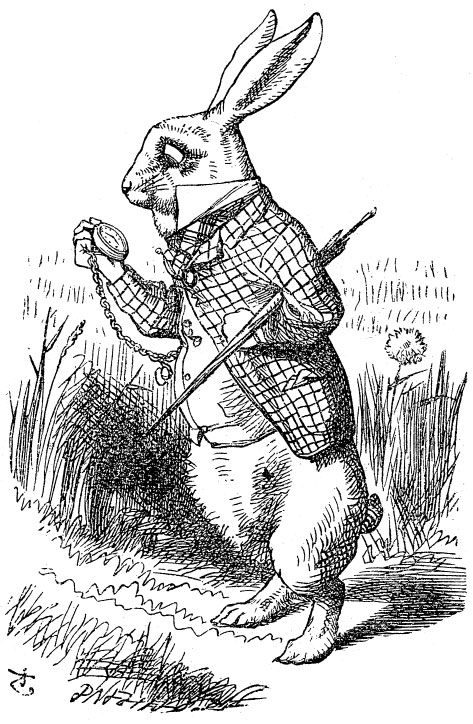
\includegraphics[width=6cm]{img/whiterabbit.jpg} \\ \medskip % Picture

\myDegree \\
\myDepartment \\
%\myFaculty \\
\myUni \\ \bigskip

\myTime\ %-- \myVersion % Time and version

\vfill

\end{center}
\end{addmargin}

\end{titlepage}
 % Main title page
% Back of the title page

\thispagestyle{empty}

\hfill

\vfill

\noindent\myName: \textit{\myTitle,} \mySubtitle, %\myDegree, 
\textcopyright\ \myTime

% You may wish to do something with the back of the title page, such as including your supervisors, location or time frame of the work. Below is an example of doing so although you may want to tweak it to your liking.

\bigskip

\noindent\spacedlowsmallcaps{Supervisor}: \\
%\myProf \\
%\myOtherProf \\ 
\mySupervisor

\medskip

\noindent\spacedlowsmallcaps{Examiner}: \\
\myExaminer

\medskip

%\noindent\spacedlowsmallcaps{Location}: \\
%\myLocation

%\medskip \\

%\noindent\spacedlowsmallcaps{Date}: \\
%\myTime
 % Back of the title page
\cleardoublepage% Dedication

\thispagestyle{empty}
\refstepcounter{dummy}

\pdfbookmark[1]{Dedication}{Dedication} % Bookmark name visible in a PDF viewer

\vspace*{3cm}

\begin{flushright}{\slshape    
No wise fish would go anywhere without a porpoise.} \\ \medskip
--- Alice in Wonderland
\end{flushright}
%\medskip
%
%\begin{center}
%Dedicated to the loving memory of Rudolf Miede. \\ \smallskip
%1939\,--\,2005
%\end{center}
 % Dedication page
%\cleardoublepage\include{FrontBackMatter/Foreword} % Uncomment and create a Foreword.tex to include a foreword
\cleardoublepage% Abstract

\pdfbookmark[1]{Abstract}{Abstract} % Bookmark name visible in a PDF viewer

\begingroup
\let\clearpage\relax
\let\cleardoublepage\relax
\let\cleardoublepage\relax

\chapter*{Abstract} % Abstract name

\noindent This thesis identifies shortcomings with how \acf{CAT} tools are developed. Their final use as an aid to translators is often not fully considered and left to others to evaluate. A unified methodology is proposed which allows a \acs{CAT} tool to be evaluated intrinsically and extrinsically using methods that show the tool's effect on the whole translation process. Special emphasis is placed on prototyping as a resource-effective way to create tools and gain critical feedback before a full implementation. To evaluate the methodology's usefulness, StyleCheck is developed and evaluated using it. StyleCheck is a tool implemented in Grammatical Framework. It detects when a style guide rule is applied and gives a hint to the translator when it isn't. The use of methods developed in \acl{TPR} generates a wealth of data that gives detailed insights into how a tool performs. Results show StyleCheck is effective at getting a style guide to be applied, more than translating from scratch or post-editing, although more work on the user interface is required. The methodology is proven to be good at coming up with \acs{CAT} tool improvements, quickly protoyping them and evaluating them.

\endgroup			

\vfill
 % Abstract page
%\cleardoublepage% Publications - a page listing research articles written using content in the thesis

\pdfbookmark[1]{Publications}{Publications} % Bookmark name visible in a PDF viewer

\chapter*{Publications} % Publications page text

Some ideas and figures have appeared previously in the following publications:

\bigskip

\noindent Put your publications from the thesis here. The packages \texttt{multibib} or \texttt{bibtopic} etc. can be used to handle multiple different bibliographies in your document. % Publications from the thesis page
\cleardoublepage% Acknowledgements

\pdfbookmark[1]{Acknowledgements}{Acknowledgements} % Bookmark name visible in a PDF viewer

\bigskip

%----------------------------------------------------------------------------------------

\begingroup

\let\clearpage\relax
\let\cleardoublepage\relax
\let\cleardoublepage\relax

\chapter*{Acknowledgements} % Acknowledgements section text

\noindent Many people deserve a big ``Thank you!'' for their help in one way or another. I'll mention a few so as not to keep readers too long from the rest of the thesis.

\medskip

\noindent Thank you:

\begin{itemize}
    \item First, to my supervisor Aarne Ranta for helpful and patient insight.

    \item Second, to all the participants in the case study who took the time to thoughtfully fill in the questionnaires and translate the texts.

    \item Last and perhaps most importantly, to all the people who asked what my thesis was about and gave me puzzled looks when I told them. After explaining it to each of them in a different way, hopefully the following pages will have found the ideal answer.
\end{itemize}    


\endgroup
 % Acknowledgements page
\pagestyle{scrheadings} % Show chapter titles as headings
\cleardoublepage% Table of Contents - List of Tables/Figures/Listings and Acronyms

\refstepcounter{dummy}

\pdfbookmark[1]{\contentsname}{tableofcontents} % Bookmark name visible in a PDF viewer

\setcounter{tocdepth}{2} % Depth of sections to include in the table of contents - currently up to subsections

\setcounter{secnumdepth}{3} % Depth of sections to number in the text itself - currently up to subsubsections

\manualmark
\markboth{\spacedlowsmallcaps{\contentsname}}{\spacedlowsmallcaps{\contentsname}}
\tableofcontents 
\automark[section]{chapter}
\renewcommand{\chaptermark}[1]{\markboth{\spacedlowsmallcaps{#1}}{\spacedlowsmallcaps{#1}}}
\renewcommand{\sectionmark}[1]{\markright{\thesection\enspace\spacedlowsmallcaps{#1}}}

\clearpage

\begingroup 
\let\clearpage\relax
\let\cleardoublepage\relax
\let\cleardoublepage\relax

%----------------------------------------------------------------------------------------
%	List of Figures
%----------------------------------------------------------------------------------------

%\refstepcounter{dummy}
%%\addcontentsline{toc}{chapter}{\listfigurename} % Uncomment if you would like the list of figures to appear in the table of contents
%\pdfbookmark[1]{\listfigurename}{lof} % Bookmark name visible in a PDF viewer
%
%\listoffigures
%
%\vspace*{8ex}
%\newpage

%----------------------------------------------------------------------------------------
%	List of Tables
%----------------------------------------------------------------------------------------

%\refstepcounter{dummy}
%%\addcontentsline{toc}{chapter}{\listtablename} % Uncomment if you would like the list of tables to appear in the table of contents
%\pdfbookmark[1]{\listtablename}{lot} % Bookmark name visible in a PDF viewer
%
%\listoftables
%        
%\vspace*{8ex}
%\newpage
    
%----------------------------------------------------------------------------------------
%	List of Listings
%---------------------------------------------------------------------------------------- 

%\refstepcounter{dummy}
%%\addcontentsline{toc}{chapter}{\lstlistlistingname} % Uncomment if you would like the list of listings to appear in the table of contents
%\pdfbookmark[1]{\lstlistlistingname}{lol} % Bookmark name visible in a PDF viewer
%
%\lstlistoflistings 
%
%\vspace*{8ex}
%\newpage
       
%----------------------------------------------------------------------------------------
%	Acronyms
%----------------------------------------------------------------------------------------

\refstepcounter{dummy}
%\addcontentsline{toc}{chapter}{Acronyms} % Uncomment if you would like the acronyms to appear in the table of contents
\pdfbookmark[1]{Acronyms}{acronyms} % Bookmark name visible in a PDF viewer

\markboth{\spacedlowsmallcaps{Acronyms}}{\spacedlowsmallcaps{Acronyms}}

\chapter*{Acronyms}
\label{ch:acronyms} % For referencing the chapter elsewhere, use \autoref{ch:acronyms} 

\begin{acronym}[PE]
\acro{CAT}{Computer-Assisted Translation}
\acro{CNL}{Controlled Natural Language}
\acro{GF}{Grammatical Framework}
\acro{HT}{Human Translation}
\acro{MT}{Machine Translation}
\acro{NLP}{Natural Language Processing}
\acro{PE}{Post-Editing}
\acro{RGL}{Resource Grammar Library}
\acro{SG}{Style Guide}
\acro{SMT}{Statistical Machine Translation}
\acro{ST}{Source Text}
\acro{TM}{Translation Memory}
\acro{TPR}{Translation Process Research}
\acro{TS}{Translation Studies}
\acro{TT}{Target Text}
\end{acronym}  
                   
\endgroup
 % Contents, list of figures/tables/listings and acronyms

\cleardoublepage

\pagenumbering{arabic} % Arabic page numbering for thesis content (1, 2, 3, etc)
%\setcounter{page}{90} % Uncomment to manually start the page counter at an arbitrary value (for example if you wish to count the pre-content pages in the page count)

\cleardoublepage % Avoids problems with pdfbookmark

%----------------------------------------------------------------------------------------
%	THESIS CONTENT - CHAPTERS
%----------------------------------------------------------------------------------------

%\ctparttext{
%\begin{flushright}{\slshape    
%The White Rabbit put on his spectacles. `Where shall I begin, please your Majesty?' he asked. \\
%`Begin at the beginning,' the King said gravely, `and go on till you come to the end: then stop.' \\} 
%\medskip
%--- Alice in Wonderland
%\end{flushright}
%} % Text on the Part 1 page describing  the content in Part 1

\part{Introduction and background} % First part of the thesis

% Chapter 1

\chapter{Introduction} % Chapter title
\label{ch:introduction} % For referencing the chapter elsewhere, use \autoref{ch:introduction} 

%----------------------------------------------------------------------------------------

\noindent Translation is the shared object of study of two research communities: \ac{TS} and \ac{MT}, which is part of the larger \ac{NLP} community. Despite this common interest, it comes as both a surprise and a concern that there is little to no interaction between these communities and their research. Each one approaches translation from a different perspective, using different methodological tools and with different aims. The most evident difference is on the definition of the object of study itself: translation. While in \ac{TS} many a pages and thoughts have been put into trying to define what translation is and how both translators as subjects and translating as a process fit together to create the final product, in \ac{MT} all this is taken for granted and nearly no thought is spared as to what it means to translate.

\acf{CAT}, where translators use computers and specialised software to help them translate, seems a natural meeting point for these two communities. Indeed, in the early days of \ac{MT} research, \ac{CAT} was proposed as the way to go in the seminal \spacedlowsmallcaps{ALPAC} report \parencite{ALPAC}, again years later by \textcite{kay1980proper} and instisted upon yet again by \textcite{kay1997still}. Despite these influential papers, only recently has strong research into \ac{CAT} started picking up. Up until now, the field of \ac{CAT} has seen the introduction of some important technologies such as the use of \ac{TM} and glossaries. Apart from these two technologies, commercial \ac{CAT} tools have mainly focused on the project management and team coordination aspects of translating.

With the recent improvement in perceived quality of \ac{MT} output, especially after the introduction of the Moses \acs{SMT} system \parencite{koehn2007moses}, \ac{CAT} now seems attractive to \ac{MT} researchers. The focus, however, has been on \acf{PE}. In \ac{PE}, the translator is charged with nothing but ``cleaning up'' a machine translation to bring it up to acceptable quality. The story goes that this approach is faster and sufficient for certain texts that don't need full human translation quality, but this is not always the case. Humans are treated as simple quality assurance mechanisms instead of as people with a certain set of skills that could be put to good use. The move to \ac{PE} seems to serve more the interests of claiming \ac{MT} is viable and economical than the interests of improving translator's working conditions.

I argue that the problems with \ac{PE} and with \ac{TM} before it --- and more generally of translation carried out between humans and computers --- arise from the compartmentalised approach to \ac{CAT} tool research and development. \ac{NLP} researchers approach the problem from their knowledge and skills, often forgetting that the systems they develop have to work well with people, a very different problem to algorithm development. Researchers can end up creating tools that not only interact poorly with translators, but also potentially work against them. Similarly, translators and researchers from \ac{TS} are also weary of the claims that a machine can do what human translators can, to the point of taking over their jobs or a considerable portion of them. To this end, numerous studies (see \autoref{ch:cat}) have tried to surface all the shortcomings of these approaches. 

This situation is not desirable for either community. What is needed is to integrate both of them and collaborate in developing \ac{CAT} tools. The basic step is to change development methodologies and move away from the current state where one community creates a tool and puts it out there, and the other has to evaluate it and pick holes in it.

This thesis proposes a research methodology (\autoref{ch:methodology}) for developing \ac{CAT} tools with a tighter-knit integration of the skills of both communities. The gist is that theoretical research in \ac{TS} and translator surveys should uncover needs which can potentially be addressed with \ac{NLP} technologies. \ac{NLP} experts can then develop a prototype technology which solves this problem. It does not necessarily have to be fully-fledged, but it should have the potential to be so. Finally, \ac{TPR} methodologies can be used to prove that this new technology actually affects translations and translators positively. If all goes well, a full implementation can be left to future research projects in academia or in commercial applications.

My hypothesis is that \ac{CAT} tools developed on the basis of the proposed methodology should generate sufficient data to allow the tool to be evaluated instrinsically and extrinsically. In order to evaluate the methodology, in this thesis I use it to develop and evaluate StyleCheck, a tool that implements style guides. The results (\autoref{ch:results}) of the tool evaluation are presented, and a metaevaluation of the methodology is discussed.

It is hoped that through the use of this methodology, \ac{CAT} tools developed in the future will be liked by translators and have a positive impact on the work they carry out. In a nutshell, \ac{CAT} at the service of translators.
 % Chapter 1
% Chapter 2

\chapter{Translation, translators and translating} % Chapter title
\label{ch:translation} % For referencing the chapter elsewhere, use \autoref{ch:examples} 

%----------------------------------------------------------------------------------------

\noindent Before delving into \ac{CAT} tools, it is best to start from the beginning and discuss what translation is. General theories of translation are estranged in \ac{MT} research. Other areas of research in \ac{NLP} base their research on theories ---~commonly linguistic theories~---, upon which models are built, implemented and tested. \ac{MT} and \ac{CAT} systems today are not explicitely built on any general theory of translation.

In this chapter, some of the main theories of translation are discussed for two reasons. First and foremost, a strong theoretical basis will reinforce research into \ac{MT}, \ac{CAT} and related technologies as well as provide a better idea of where they should be heading and what can be improved. Having an explicit starting point for research can clear the way for competing theories to emerge and develop their own lines of research if considered necessary. 

Second, \acf{TPR} research (\autoref{sec:tpr}) ---~part of theoretical research into translation~--- provides a useful set of methodological tools. These tools will be used in this thesis and integrated into the proposed research methodology (\autoref{ch:methodology}).

% TODO Get rid of the following paragraph?

%Also, it is worth noting that the output of \ac{MT} systems has improved considerably in recent years, leading to a focus on attaining ``quality'' translations as the next step up from gisting systems. Defining quality, measuring it and creating metrics useful for \ac{MT}, \ac{PE} or even \ac{HT} is an active and ongoing field of research. It is thus natural to turn to \acf{TS} and the theories it has developed ---~which have been dealing with the notion of ``quality'' and the very essence of what translation is for a long time~--- to see if answers that jointly describe \ac{MT} and \ac{HT} can be found.

\section{Overview of paradigms in Translation Theory}
\label{sec:paradigms}

\noindent This section provides a high-level overview of the main paradigms in translation theory. They are taken as per \textcite{pym2009exploring}, who describes five basic paradigms. Together they cover most of the individual theories of translation that have been proposed over the years. 

\subsection{Theories of Equivalence}

\noindent The equivalence paradigm postulates that there is an equalness of value between the \ac{ST} and the \ac{TT} at some level. This paradigm relies heavily on linguistics, as can be seen in the work of \textcite{catford1965linguistic}, who postulated different possible equivalence levels for a \ac{ST} and a \ac{TT}: phonetic, lexical, syntactic, etc.

More generally, the focus in the theories of equivalence is placed on the \ac{ST}, which guides and establishes what will appear in the \ac{TT}. Translation is thus understood in the sense of creating a \ac{TT} which is equivalent to the \ac{ST} and contains nothing but the \ac{ST} (save clearly delimited translator's notes). This is the notion that is the most widespread amongst the general public and \ac{MT} research.

\subsection{Skopos or Functional Theories}

\noindent Skopos theory (from the Greek \textit{skopos} `aim', `intention') introduced a radically new idea in translation: what matters when translating is the purpose, the function that the \ac{TT} has to fulfil \parencite{holz1984translatorisches,reiss1984grundlegung}. This theory escaped from the constraints of linguistics and the \ac{ST} to enter the real world, where translators carry out translations according to customers' requirements. Large variations in the \ac{TT} are acceptable if justified by the function that the \ac{TT} has to fulfil, which is often different from that of the \ac{ST}. Equivalence is thus relagated to the case where the function is the same for the \ac{ST} and the \ac{TT}. 

One of the most profound implications of this theory is that the reasons for choosing to translate a \ac{ST} in one way or another cannot be found in linguistics, they are found in communication, ethics, sociology, marketing, etc. This lead to the appearance of agents in the paradigm, \ie the customer, the employer, users of the translation, etc. For some theoreticians, the main agents in this paradigm are the translators, since they are the ones who have the final word on decisions that have to be made and other agents simply collaborate in this task \parencite{reiss1984grundlegung}. For others, the focus is more on the client's requirements and not on the translator's individuality \parencite{nord1997translation}.

\subsection{Descriptive Theories}
\label{sub:descriptive}

\noindent Descriptive Translation Studies, developed in parallel to skopos theories, again presented a breakwaway from previous theories. In this paradigm the notion of ``assumed translations'' \parencite{toury1995notion} takes centre stage: all translations are equivalent due to them being considered a translation. Thus, the aim is to observe originals and translations and describe how they differ and what makes them equivalent rather than prescribing a certain type of equivalence or a need to adapt to the \ac{TT} function as the only valid ways to translate.

One of the main notions in the descriptive paradigm is that of norms, whose main proponent is \textcite{toury1995nature}. Translations are seen to be produced within a certain culture and society, and at a certain time in history. Norms turn the ideas and values within a society into ``performance instructions'', \ie\ what can or cannot be done, what is permissable and what isn't \parencite{toury1995nature}. Translators will thus adopt different strategies and produce different translations according to the society and historical time they live in. The notion of norms can lead to prescriptivisim: discovering the relevant norms allows for translations to be classified as good or bad depending on whether they follow the norms of a certain time and society. Thus, the notion of norms can lead back to the presciptivism it was trying to escape. 

\subsection{Theories of Indeterminacy}

\noindent The paradigm of indeterminism questions many of the assumptions of the other paradigms, and even the existance of translation itself. The principle of indeterminacy \parencite{quine1969linguistics} postulated that it is impossible to know the real meaning of an utterance, there are always other possible interpretations based on the same empirical evidence. In translation, this led to the view that there are always many possible ways to translate a text and it is impossible to be certain that any one of them is right or is equivalent to the ``meaning'' of the \ac{ST}. We can always construct hypotheses to defend one interpretation or another, all of which can be supported by the same empirical evidence, \ie the \ac{ST} \parencite{quine1969linguistics}.

\textcite{pym2009exploring} groups various related but somewhat different theories in this paradigm. A full overview is not within the scope of this thesis, but the notion of ``abusive fidelity'' \parencite{lewis1985measure} is one worth mentioning. One of the problems with indeterminisim is that it doesn't provide translators with ways of carrying out their work. The closest there is to a guideline is to ``abuse fidelity'' and translate the key points within a text as close as possible to the \ac{ST}, to the point of making the \ac{TT} sound strange to the target culture \parencite{lewis1985measure}. Thus, users are made aware of the translation itself by breaking the illusion of equivalence or symmetry between languages \parencite{snell1988translation}, the illusion that a universal transfer of meaning is possible.

\subsection{Localisation}
\label{sub:localisation}

\noindent \textcite{pym2009exploring} introduces and describes localisation as a new paradigm in \ac{TS}. The process of localisation ---~translating a product into different locales~--- introduces three important concepts. First, the idea of locale, which combines both a language and a specific culture. For example, Spanish can be divided into the Spain-Spanish locale, the Mexico-Spanish locale, etc. Second, internationalisation as the process of adapting a \ac{ST} so that it can be easily translated into various locales. This entails the creation of an intermediate product that is either augmented (more space for strings, adding date formatting options to software, etc.) or simplified through the use of a \ac{CNL}.

Third, \textcite{pym2009exploring} cites the rise of non-linear texts, which are often those that are localised. Non-linear texts are neither translated nor used from beginning to end. Rather, fragments are used such as the various strings in a piece of software, parts of a reference manual for software or appliances, etc. These products are usually incrementally updated, meaning that future translations are simply the new or modified segments of the product. It often occurrs that these segments are presented to translators with little to no context as to where they are to appear in the final product.

The three previous factors bring about a change in the way translators work. Translation is but a single step in a larger process consisting of internationalisation, translation, editing and quality assurance. Translation is reduced to an artificial kind of equivalence weighed down by the importance of reuse and accepting \acl{TM} suggestions or terminology from glossaries (even though translators may consider them wrong or inadequate), with little incentive for translators to want to improve it \parencite{pym2009exploring}. \textcite{esselink2002localisation} notes that translators should carry out other steps in the localisation process, such as internationalisation and final editing, for which their intercultural skills are very useful and relevant.

\section{MT: Translation as a Distributed System}
\label{sec:mt_theory}

\noindent The paradigms presented in the previous section are but a brief glimpse of all the opinions and theories that have been proposed about translation, but a detailed review of them is outside of the scope and aim of this thesis\footnote{For further details, \textcite{pym2009exploring} provides a thorough discussion of each paradigm, its authors, its pros and cons and its authors.}. What they do provide is a good basis for discussion of \ac{MT} and how it fits in and relates to the paradigms.

\textcite{pym2009exploring} places \ac{MT} in the equivalence paradigm, albeit a new kind of equivalence that serves the higher goal of reuse. Looking at the methods \ac{SMT} uses today, this would seem to be the case. A large corpus of translated texts are collected, aligned at the sentence level, broken down into phrases or syntactic structures, aligned again and probabilities are calculated. Texts to be translated are then broken down into sentences and these pieces are then reused to create the \ac{TT}. Just as was the case in the theories of equivalence, the \ac{ST} rules the roost: it is the main element that guides what appears in the \ac{TT} and linguistics is all that matters. \textcite{kay1997still} also shares this view of \ac{MT}, as the following passage ---~which still rings true today~--- shows:

\begin{quote}
    Workers in this field [\textit{\ac{MT} research}] usually take it as self-evident what constitutes a translation, especially within the relatively limited domains in which automatic methods might be applied. In particular, it is assumed that the sequence of sentences that make up the translation should preserve the intended meanings of the corresponding sentences in the original. \\
--- \textcite{kay1997still}
\end{quote}

\noindent \textcite{culo2014approaching} characterises \ac{MT} as being instrumental and aiming to be functionally constant. Thus, \ac{MT} is still stuck in the equivalence paradigm, but limited to cases where the \ac{ST} and \ac{TT} functions are the same. The problem arises when considering the corpora that \ac{SMT} systems are based on: since they will have been translated by different people, from different sources and for different purposes, can we be certain that what resulting translations will be functionally identical? What is more, statistical systems will choose the most probable translation options from this amalgama, can probability really guarantee functional equivalence? From the point of view of descriptive theories, it might well be that the most probable translations that \ac{SMT} generates correspond to translation norms present in the parallel corpus used. If, for example, a corpora of 19th century texts were fed to an \ac{MT} system, the resulting translations might make use of the translation norms of the time. But then again, the very process of breaking down sentences into phrases or syntactic structures and rebuilding them might water down the norms and generate some other \ac{SMT} intrinsic norms. Studies would be required to determine if this is the case.

If we take a wider view, we can see that \ac{MT} does indeed use skopos theory. The techniques of domain adaptation and the use of in-domain data imply that the \ac{MT} developer is thinking about the users of the \ac{TT} and modifying what the \ac{MT} system should output accordingly. Translators change their translation strategies in order to adapt the \ac{TT} to the target culture. Since changing the \ac{MT} system is costly and can involve much research and effort, the next best approach is used to adapt the \ac{TT}: use data that closely resembles it. The methods and results are different, but the aim is the same. This implies that linguistics (or its statistical proxy) is not the be-all and end-all in translation, but that external factors have to be taken into account. 

One final point to note about the previous discussion is the return to a human. Trying to understand \ac{MT} from a theoretical perspective forces us to step back from the system itself with its mathematics or rules and into the human realm where we can attribute intelligent phenomena such as intentionality and thought. In the case of \ac{MT}, it is the system developers and system implementers that have stepped into the shoes of translators and have to carry out the translation. Instead of doing it all themselves, they proxy the work to computers: a set of rules or a parallel corpus takes the place of memory, mathematics and algorithms take the place of translation strategies and procedures. This view rings close to what \textcite{pym2009exploring} describes for the localisation paradigm: splitting what a single translator used to do alone into parts that are performed by different people or even computers. In other words, translation as a distributed system. \ac{MT} is simply the expression of translation where the majority of those parts are taken over by a computer.

\section{Translation Process Research}
\label{sec:tpr}

\noindent \acf{TPR} is a theoretical branch closely related to descriptive translation studies (\autoref{sub:descriptive}) that aims to describe how translators translate. It focuses on aspects such as translation units, styles, phases, variation among translators, etc. Essentially, it provides a detailed description of how a translation is carried out by a translator, not just a description of the final text itself. 

\textcite{christensen2011studies} provides an overview of the cognitive grounding for translation and \ac{TPR}, a brief summary of which now follows. Some aspects of the translation process can be observed directly, but a large part of it occurs in a translator's mind. To understand the translation process better, we need to access the cognitive phenomena that go on in the mind. \textcite{risku2010cognitive} notes that cognition is not only a mental affair, the environment plays a direct role in the thought processes. So, understanding translation requires observing what goes on in the mind as well as what goes on in a translator's work environment. \textcite{hutchins2000distributed} proposes the Distributed Cognition Paradigm, in which cognition is distributed across people and artifacts that make humans smarter. In other words, we think with our minds and with our tools, artifacts which can change and shape our mental processes. Thus, when developing tools for translators it becomes relevant to see how they affect their mental processes, and not just the final translation.

In order to gather data on the cognitive processes that go on in the mind, several methodologies exist. \textcite{christensen2011studies} provides a detailed classification and description of the positive and negative aspects of each. A first major distinction is whether the data is collected after the translation (offline) or as the translation is being carried out (online). Within each group, two further subgroups can be defined. Offline methods can include those that analyse the product (\ie, the translations) or verbal-report data (such as retrospective questionnaires). Online methods can include behaviour observation (eye tracking, keylogging, screen recording, etc.) and verbal-report data (such as think-aloud protocols, where translators say what they are doing while they are doing it). A detailed description of each is outside of the skope of this thesis, but the differences mainly relate to how much each method affects and can potentially alter the process it's trying to observe and how reliable the data gathered is. To overcome the potential downfalls of any one method, triangulation is used. Triangulation \parencite{alves2003triangulating} means collecting data using more than one of the methods previously described in order to contrast and complement the obtained data, gaining a better view of the overall picture.

Many recent studies have used \ac{TPR} to study translation and translation tools such as translation memories and \acl{PE}. Keylogging and eyetracking \parencite{obrien2009eyetracking} have been particularly popular. Databases have been created in an effort to standardise the collected data and allow for experiments on large datasets to be carried out, such as the \spacedlowsmallcaps{CRITT TPR-DB} \parencite{carl2012critt}. This thesis will follow in these footsteps at a smaller scale using some of the more basic \ac{TPR} methods (those that don't require specialised hardware), as will be discussed in \autoref{ch:experiment}.
 % Chapter 2
% Chapter 3
\chapter{Computer-Assisted Translation} 
\label{ch:cat} 

%----------------------------------------------------------------------------------------

\section{Man, Machine and Everything In-Between}

\noindent Let us place translation on a linear continuum. On one end sits \ac{HT}, performed by human translators from scratch. However, this does not mean that they don't use computers to search online dictionaries, databases, websites, articles, style guides, help forums and a plethora of other resources. They do, and it is an integral part of the tasks a translator carries out. 

On the other end of the continuum sits \ac{MT}, perfomed by machines without human intervention. However, this is only partly true. The most widespread type of \ac{MT} systems today, \ac{SMT} systems, rely on huge corpora of aligned texts previously translated by human translators. Even rule-based systems rely on the human thought put into building the rules. Just like skopos and descriptive theories grounded translation into the real world as an activity carried out by people, away from the abstract equivalence paradigm, the same can be done for \ac{MT}. As described in \autoref{sec:mt_theory}, \ac{MT} does not carry out translation in a platonic world of ideas and $argmax$es, but someone in the real world designs the systems and someone uses them to translate texts for a certain purpose. Thus it is clear that our linear continuum is not as black and white, man vs. machine, as it first seemed.

%------------------------------------------------

\subsection{Current State of CAT Tools}

\noindent Somewhere in the middle of the continuum, closer to \ac{HT} than \ac{MT}, sit \ac{CAT} tools. These provide a wealth of features to help translators carry out their translations. The most widely-used of these tools today is Trados\footnote{\url{http://www.translationzone.com/trados.html}}. In 2006 a survey of language professionals reported that 76~\% of its respondents used it \parencite{lagoudaki2006translation}.

The main feature of \ac{CAT} tools are Translation Memories (\acsp{TM}). A \ac{TM} is a database of a translator's previous translations, segmented into sentences and aligned. When a translator has a new text to translate, each sentence-segment in the \ac{ST} is string matched against those in the \ac{TM} database. If a match is found above a pre-determined threshold of similarity, the match is presented to the translator as a suggested translation for the current segment. This tool is especially useful when translating updates to manuals or other similar text types, where the majority of sentences have already been previously translated.

Similarly, glossaries of bilingual terms can be created and function in much the same fashion as a \ac{TM}, but for smaller units such as words or multi-word units. Recent research has focused on augmenting \ac{TM}s by including smaller subsentential units, effectively combining them with glossaries. For example, \textcite{chuang2005collocational} present a method to extract collocations from corpora and build \ac{TM}s out of them.

Some of the other main features of \ac{CAT} tools are related to project management, especially for localisation, where texts are frequently non-linear (as discussed in \autoref{sub:localisation}) and can come in many formats that are difficult to handle for a translator, such as \spacedlowsmallcaps{HTML, XML} and others. \ac{CAT} tools extract the strings to be translated and present them to translators in a consistent interface, usually a two-column window of cells: in one column the \ac{ST} segmented into sentences and in the other textboxes waiting for the translation of the corresponding segment. Some \ac{CAT} tools also enable easy collaboration between teams of translators, allowing them to work on a shared \ac{TM} and glossary hosted on a server.

Recently, research into \ac{CAT} tools has picked up. For example, the open-source tool MateCat \parencite{federico2014matecat} has been developed in an effort to integrate \ac{MT} and \ac{CAT} tools, moving futher towards setting \ac{PE} as the norm. 

%------------------------------------------------

\subsection{Problems With CAT Tools}

\noindent Despite the many advantages of \ac{CAT} tools presented in the previous section, numerous studies have identified problems, especially with regards to the way translators translate when using them and how it effects their mental processes. \textcite{christensen2011studies} provides an overview of a number of studies into \ac{TM} usage and their effects on translator cognitive processes, some of which are discussed below.

\textcite{dragsted2004segmentation,dragsted2006computer} found that translators don't mentally segment into sentences, but rather tend to use phrases and clauses. This clashes with the sentence segmentation that \ac{TM} forces. A further finding was that translators using a \ac{TM} tended to revise sentence by sentence as they go along rather than carrying out a whole global revision at the end as they would when not using one. 

\textcite{christensen2011impact} investigated the effect of \ac{TM} on students right after they used \ac{CAT} tools for the first time. Students reported that the technology was useful but also deceptive, since they felt they lost control of the process, lost track of the aim of the translation, etc. They also reported that translation become mechanical and much less creative and functional. 

Moving away from the mental process of translators and looking at the translations themselves, \textcite{jimenez2010effect} carried out a contrastive analysis of web texts localised using a \ac{TM} and texts spontaneously produced in the source language. He found that differences in the text superstructure are present, indicating the source text structure was being closely replicated. Texts translated with a \ac{TM} also showed lower levels of lexical and typographic consistency. However, he does note that \ac{TM} is probably only one of many factors that combined to produce the observed differences.

%----------------------------------------------------------------------------------------

\section{Post-Editing Machine Translation}

\noindent Coming back to the continuum introduced at the beginning of this chapter, \acf{PE} sits close to the \ac{MT} end. \acl{PE} consists in having translators edit a translation produced by an \ac{MT} system in order to improve its quality. Recently, \ac{PE} has gained importance both in research and in industry usage. \textcite{carl2015post} claim that the recent surge in interest is due to the rise in demand for translation and the inability for human translators to keep up with this demand.

\textcite{carl2015post} propose different types and quality levels for post-editing, ranging from light \ac{PE} aimed at changing only what is necessary for text comprehension, and full \ac{PE} aimed at bringing \ac{MT} output to the quality produced by a human translator. However, as the authors discuss, this has an impact on translators as it is difficult to ask them to produce a translation they consider to be of low quality, generating a negative attitude towards \ac{PE}. Most research into \ac{PE} revolves around the light variant, with little attention being paid to ``full \ac{PE}''. 

\textcite{carl2015post} also conducted a study with translators, revealing that 83~\% of participants would have preferred to translate from scratch rather than use \ac{PE}. Some authors have argued for the need to teach \ac{PE} as a separate skill in order to familiarise students with the workflow and expectations \parencite{obrien2002teach}. It is not clear, however, if the approach of adapting translators to the tools is a better way forward than adapting the tools to the translators.

%----------------------------------------------------------------------------------------

 % Chapter 3

\cleardoublepage % Empty page before the start of the next part

%------------------------------------------------

\ctparttext{} % Text on the Part 3 page describing the content in Part 3
\part{A Unified Methodology} % Third part of the thesis
% Chapter 4

\chapter{CAT Research Methodology} % Chapter title
\label{ch:methodology}

\noindent Developments in the field of \ac{CAT} such as those mentioned in the previous chapter have been created without an extensive study into the potential effects they have on translators. While reuse, speed and ---~increasingly~--- reduced cognitive effort are claimed as advantages of each new improvement, studies have brought to light the not-so-obvious influences these tools have on the translation process, on translators and on translations themselves. Given that \ac{TM} and \ac{CAT} tools in general are now an essential part of a translator's environment \parencite{o2012translation}, it is probably time to think through what approach to take when developing further improvements.

A common theme of the \ac{CAT} tools discussed in the previous chapter is that they weigh down human translation with their own inherent limitations and simplifications. As seen in \autoref{sec:mt_theory}, the fact that \ac{MT} is basically stuck in the equivalence paradigm can be seen as both a limitation and simplification: trying to include all the external variables into the models used by \ac{SMT} systems would most likely make the problem intractable. \textcite{hardmeier2014discourse} elaborates on translation theories and some of the simplifications \ac{SMT} adopted and still adopts to solve the translation problem computationally. \textcite{hardmeier2014discourse} discusses two notable examples: the existence of some kind of equivalence between the \ac{ST} and the \ac{TT}, which enables the notion of word alignments between a \ac{ST} and its \ac{TT}; and translating only one sentence at a time without considering the wider textual context. These design limitations are now burdened onto translators through \ac{PE} and \ac{TM}s (even more so now that research into unifying \ac{TM}s and \ac{MT} is picking up).

It is of no surprise that translators tend to dislike using these tools, given that they make their work mechanical and less creative \parencite{christensen2011impact}. Taking a finer-grained look at \ac{PE}, the very term post-edit seems to convey the idea that the hard work is already done by the system, and just some cosmetic changes are required.

Evaluation of \ac{CAT} tools is an essential point that needs addressing. Currently, many studies draw conclusions simply based on speed and cognitive effort measured as words processed per unit of time \parencite{carl2015post}. I argue that not all effort is created equal. Translators carry out various kinds of tasks when translating, some which require skills aquired after years of practice and study. It is natural that translating a play on words, a complicated syntactical structure, an unclear passage in the \ac{ST}, etc. requires more effort and time than other tasks. These are precisely some of the tasks human translators should be carrying out and are trained to carry out. Offloading key tasks such as word and structure selection to an \ac{MT} engine and using qualified translators to ``clean up'' the output is a questionable way forward. As was discussed in \autoref{ch:cat}, this leads to negative attitudes towards \ac{PE}.

I propose a new approach to the development of \ac{CAT} tools that puts translators first from the outset. The methodology consists of the following steps:

\begin{enumerate}
\item \textit{Gather automation candidates:} theoretical work carried out in \ac{TS} and translators themselves through surveys are a valuable source of candidate taskes to be automated. They can provide hints as to which tasks within the translation process are the most tedious and can potentially be carried out without human intervention.
\item \textit{Select candidates addressable by \spacedlowsmallcaps{NLP}:} from the candidates gathered above, experts in computational linguistics can select the ones that can be resonably carried out with \spacedlowsmallcaps{NLP} tools. Other areas that plain software engineering can deal with could also be identified. 
\item \textit{Develop a tool or prototype:} design and implement a system to carry out the selected task. Emphasis is placed on prototype: at this stage, a full implementation may not be required as long as it can be reliably given to translators to use in the context of an experiment. Prototyping allows the tool development process to go much faster, quickly discarding bad ideas and gathering key feedback to improve the prototype once it is time to implement a full system. It could be argued that any difficulties in implementing a full system have not been caught. But in that case the design and efectiveness of the tool has been tested in a real setting and it justifies more resources being spent on overcoming the implementation difficulties. The opposite case, a good system that doesn't mix well with translators, is undesirable.
\item \textit{Intrinsic tool evaluation:} depending on the nature of the tool and whether it is a full tool or a prototype, an intrinsic evaluation should be carried out. At the very least, it should show acceptable performance in the experimental setup described in the next step.
\item \textit{Extrinsic evaluation:} an experimental setup is designed for translators to use the tool. Usage data is obtained by means of triangulation of data-gathering methods developed in \ac{TPR}. A good mix of methods (online and offline, verbal-report, product analysis and process monitoring) is preferable. The data gathered should then allow evaluation of the tool's effects on the whole translation process, including translators. The aim will be to answer the question ``Does this tool help translators carry out their work?''.
\end{enumerate}

The previous methodology should generate tools which do not force limitations onto translators and negatively affect their normal workflow. It is important to stress that the proposed methodology is designed for \ac{CAT} tool development. The idea of a prototype forces the researcher to not go down the rabbit whole of developing a perfect system. It instead forces them to take a step back and spend less time on the tool itself and more on how the tool is used and if it makes sense for translators. This approach is clearly not ideal for the development of a parsing algorithm, for example. \ac{CAT} is an eminently practical affair and the development of \ac{CAT} tools should reflect this fact.
 % Chapter 4
% Chapter X

\chapter{Experiment Overview} % Chapter title
\label{ch:experiment}

%----------------------------------------------------------------------------------------

\section{General Hypothesis and Evaluation}

\noindent As stated in \autoref{ch:introduction}, this thesis formulates the following hypothesis:

\begin{quote}
\paragraph{Hypothesis:} The methodology laid out in \autoref{ch:methodology} will allow \ac{CAT} tools to be developed and evaluated based on how well they perform intrinsically as well as extrinsically with translators.
\end{quote}

\noindent In order to evaluate the methodology, a case study was used. Specifically, a \ac{CAT} tool called StyleCheck was designed and evaluated. Then, a metaevaluation of the methodology is carried out. To sustain the hypothesis, the methodology should:

\begin{aenumerate}
    \item Allow for a \ac{CAT} tool to be developed and evaluated with translators in mind. Specifically, it should show effects of the tool on the whole translation process (product, process and agent; translation, translating and translator). 
    \item Provide tools that generate sufficient data for the tool to be evaluated as laid out before.
\end{aenumerate}

%------------------------------------------------

\section{Online Experiment}
\label{sec:online}

\noindent StyleCheck was develiped for the case study, a tool to check if style guide rules are applied in a text and give translators a suggestion if they aren't (see \autoref{ch:stylecheck} for details). A special website was created to allow StyleCheck to be evaluated by translators. This allowed participants to work from their own computers in a setting familiar to them. The Spanish Wikipedia style guide was chosen and three text fragments were selected to be translated from English into Spanish. Three setups in which to translate the text were devised:

\begin{enumerate}
    \item \textit{Translation from scratch} (\spacedlowsmallcaps{scratch}): The text was translated from scratch without any \ac{CAT} tool assistance. Translators were free to translate as they normally would, including searching on the Internet and in databases for translations, finding more information about the text topic, etc.
    \item \textit{Post-Editing} (\ac{PE}): A machine translation of the text provided by Google Translate\footnote{\url{https://translate.google.com/}} was given to participants. So as to avoid negative connotations that Google Translate may have for translators, they were simply told the suggestions came from an \ac{MT} engine without specifying which one. \textcite{carl2015post} provided participants in their study with a set of guidelines for how to post-edit. No such guidelines were offered in this experiment, instead opting to give translators freedom to use the suggestions as much or as little as they wanted.
    \item \textit{Translation using StyleCheck} (\spacedlowsmallcaps{style}): In this setting, when a participant finishes translating a sentence and moves to the next, the previous sentence is checked using StyleCheck and any returned style hints are presented to the participant. Translators can then choose to follow the style hint or ignore it.
\end{enumerate}

In order to obtain varied data, the text and setup combinations were shuffled. This created six combinations that ensured each text was translated twice in each setup. Thus, the minimum number of participants required for the experiment was six.

Participants were gathered through the Internet. A call for participation in the experiment was posted in various translation-related Facebook groups whose participants are mostly translators or translation students. Participants were asked to contact an email address to request a unique participation link. It was hoped that this approach would limit the number of participants who abandoned the experiment half-way through, as they had implicitely commited to carrying it out. This was especially desirable given that each participant was given a different text-setup order and all possible combinations needed to be covered with the minimum number of participants. If the website had generated the order and Participant \spacedlowsmallcaps{ID} automatically, a high rate of abandonment or curious people clicking through a couple of pages may have ended with results not covering all possible text combinations and being skewed.

Participants did not receive payment or other kinds of compensation for their participation in the experiment due to the lack of funding available for this thesis. This could influence the results as translators may be inclined to put less effort into the translations if they don't receive any compensation. Ideally, experiments with translators should include payment in line with market prices so that they feel they are translating as they would with a normal client.

Following the proposed methodology, the StyleCheck tool is evaluated using \ac{TPR} methodologies. Despite many advanced monitoring tools such as eye-trackers and screen recording being used today, this thesis takes a simpler approach. The online website format used for the experiment limits the hardware capabilities to participants' own computers and limits the software to what can be acheived with a small server and web browser combination.

Both online and offline methodologies were used. The online data recorded is detailed in \autoref{sec:logging} and was collected on the server. Offline verbal report data was also collected through the use of retrospective questionnaires. Offline verbalisation does not affect the task and subject's mental processess as much as online methods do (for example, think-aloud protocols). The downside of verbalisation is that if the process to be observed (e.g. \ac{PE} or using a \ac{TM}) has become routine, the steps to perform no longer live in the short-term memory and are thus not accessible through verbalisation. This can have an impact if the participants have extensive previous experience with the task to be carried out. 

Finally, the collected data was analysed and contrasted in order to see if the hypotheses could be strengthened.

%------------------------------------------------

\section{Case Study: Wikipedia}

\noindent Wikipedia was chosen as the subject for the experiment case study, since it contains freely available texts and also has style guides for various languages. First, an imaginary translation brief was created so that participants could use it as a guide for their translation choices:

\begin{quote}
Wikipedia set up a crowdfunding campaign in an effort to pay for some professional translations of articles very popular in different regions of the world. After a huge success, they invited applications from translators. You applied and have now been selected to translate three articles from English into Spanish. Wikipedia has reminded you of the global nature and scale of the project and has provided \href{http://es.wikipedia.org/wiki/Wikipedia:Manual_de_estilo}{a link to its style guide} in order to help you translate.
\end{quote}

The brief included a link to the Spanish Wikipedia Style Guide. Clicks on this link by participants were logged (see \autoref{sec:logging}). The three texts used for the experiments can be found in \autoref{app:texts}. After an in-depth look at the style guide, the texts were chosen following three criteria:

\begin{itemize}
\item The text subject matter should not be specialized.
\item Various style rules could apply to the text.
\item The text should not present major translation problems that would require a lot of time and research to solve.
\end{itemize}

The texts will be referred to as \ai, \charlotte and \garfield in the rest of this thesis.
 % Chapter 6
% Chapter X

\chapter{StyleCheck: A Tool to Apply Style Guides}
\label{ch:stylecheck}

%----------------------------------------------------------------------------------------

\section{Style Guides}

\noindent Following the proposed methodology, translation theory was used as a basis to develop a \ac{CAT} tool that implements a \ac{SG}. \acp{SG} are collections of rules that serve to standardise linguistic content \parencite{vidal2013guia}. Within a language, many different ways of writing or expressing an idea exist. From the wide range of possibilities, dialects choose a subset, as do specific domains, genres, language academies and even individuals. Style guides aim to define a subset of language for use in a specific domain (such as style manuals for scientific writing) or most commonly for a specific entity \parencite{vidal2013guia}. In the latter type we can place \acp{SG} from the European Union, from Wikipedia or from newspapers and other publications. The idea is to guarantee that texts written by different authors conform to a set of rules so that they can be recognised as coming from a single entity, creating a specific ``voice'' of sorts. 

Style guides can be more or less restrictive, \ie aim to cover a larger or smaller subset of linguistic phenomena that need to be standardised. \aclp{CNL} can be considered an extreme form of \acp{SG} where basic syntax and constructions of a language are defined. Style guides tend to focus on formal aspects (such as punctuation and formatting), lexicon, specific linguistic constructions, etc. 

Style guides are essentially made up of rules. The structure of these rules is to identify a specific linguistic element (word, punctuation, structure, meaning, etc.) and offer the one or more ways in which it should be expressed, often giving examples of the ways in which it should not be expressed \parencite{vidal2013guia}. Thus, to apply style guide rules digitally requires a system that can detect the specific linguistic element and is able to transform it \parencite{vidal2013guia}.

It is worth mentioning that many style guides also include information not directly related to linguistic standardisation, such as legal considerations for journalists, encyclopaedic knowledge about a certain topic, how to use company software or insert certain symbols into a Word document, etc. This evidences the informal nature of style guides and the multiple aims they sometimes try to serve.

Style guides are an important skill a translator should learn as they are widely used when translating \parencite{washbourne2012style}. A problem for translators is that they may have to handle many different style guides, each for a specific client. In this context, it is easy to mix-up the rules or simply not bother reading through a large style guide for a small job: the time that would be invested in learning the guide's rules would far exceed the time spent on the translation itself. The proof-reader is then charged with ensuring style guide rules are applied during the revision phase.

StyleCheck aims to solve the problem. As translators work on a text, they will be offered suggestions when rules contained in a style guide haven't been applied. Then, they will be able to immediately solve the problem by applying them, which will reduce the time needed for proof-reading and the time spent learning a style guide.

%----------------------------------------------------------------------------------------

\section{Grammatical Framework}

\noindent StyleCheck is implemented using \ac{GF} \parencite{ranta2011gf}. \ac{GF} is a programming language and grammar formalism used to build multilingual grammar applications. \ac{GF} draws heavily from functional programming and from type theory. The real strength of \ac{GF} is the \ac{RGL} \parencite{ranta2009rgl}, which implements basic morphology and syntax for a number of languages. The \ac{RGL} provides a common, high-level \spacedlowsmallcaps{API} to use the syntax, allowing for fast multilingual application development. Relevant for StyleCheck is \ac{GF}'s tried and tested use in the field of \ac{CNL} \parencite{angelov2009cnl,kaljurand2013wiki,ranta2014embedded}.

Grammars in \ac{GF} are split into two parts: the abstract syntax and the concrete syntax. The abstract syntax is intended to represent semantics, while the concrete syntax (one for each language) links the abstract syntax to a particular string representation. More specifically, functions defined in the abstract syntax are mapped to linearizations in the concrete syntax. 

As an example, the abstract syntax funcion

\begin{lstlisting}[numbers=none]
fun AvoidSeasons_Hint : StyleHint ;
\end{lstlisting}

%\begin{minted}
%fun AvoidSeasons_Hint : StyleHint ;
%\end{minted}
%
%\begin{minted}{tex}
%fun AvoidSeasons_Hint : StyleHint ;
%\end{minted}

\noindent builds a record of type \texttt{StyleHint}. In the Spanish concrete syntax, this would be realised as:

\begin{lstlisting}[numbers=none]
lin AvoidSeasons_Hint = mkStyleHint "verano" "Don't use seasons";
\end{lstlisting}

\noindent where a \texttt{StyleHint} is a record built out of a season ``verano'' and the suggestion ``Don't use seasons''. When ``verano'' is encountered during parsing, a \texttt{StyleHint} is built and mapped to the abstract syntax function \texttt{AvoidSeasons\_Hint}. Then, from the abstract syntax tree representation a different concrete syntax can take the abstract function that was matched in the text and select from it only the suggestion text, which can then be output to the user.

This is a simplified view of how StyleCheck is designed, but it serves to illustrate the main idea: a text is parsed and any detected style rules are mapped to a style suggestion.


%----------------------------------------------------------------------------------------

\section{StyleCheck}

%------------------------------------------------
\subsection{Development Procedure}

\noindent The StyleCheck grammar was developed as follows. First, from each text to be used in the online experiment all Wikipedia style guide rules that could be applied to it were identified. Since the style guide refers to the Diccionario Panhispánico de Dudas \parencite{real2005dudas} for aspects not specifically mentioned in the style guide, it too was checked. The obtained rules were then classified as rules, hints or lookups in the following manner:

\begin{itemize}
    \item \textit{Style rules:} linguistic elements that have more than one possible forms, out of which one or more forms are approved by the style guide. For example, the correct spelling in Spanish of the capital of \spacedlowsmallcaps{UAE} is ``Abu Dabi'', not ``Abu Dhabi'' as in English.
    \item \textit{Style hints:} linguistic elements whose approved form is not self-evident and requires reasoning. Through the use of a suggestion, the translator can be made aware of the issue and decide whether action needs to be taken or not. For example, the Wikipedia style guide recommends not temporally locating events using only seasons, as the months they refer to differ in the Northern and Southern hemisphere of the Earth. In this case, all mentions of a season would trigger a suggestion for the translator to check this aspect.
    \item \textit{Style lookups:} the third possibility that was contemplated were style lookups. For some elements that have many possibile uses, such as full stops, commas or slashes, showing a suggestion every time they appear as would be the case with a style hint was deemed to be too annoying. Instead, style lookups would allow the translator to select one of these common elements and be taken shown the full range of possibilities. Thus, the translator would only lookup these elements on-demand, when he or she would consider it necessary.
\end{itemize}

Given that only one rule was classified as a style lookup (the use of the forward slash symbol), it was decided to apply it as a style hint instead and leave the lookup framework at the theoretical design stage to be implemented in future work. The forward slash only appeared once in one of the texts, so it didn't risk being annoying as would be the case if it were a comma or a full stop.

Rules were implemented as a record with fields for optional forms, approved forms and the hint (\autoref{lst:records}). Style hints and lookups contained all the fields in a rule, except for the \texttt{approved} field. All of these fields were of type \texttt{Chunk}, which is simply defined as a string.

\begin{lstlisting}[caption={Record structure for the rule types},label=lst:records]
StyleRule = {approved,options,hint : Chunk} ;
StyleHint = {options,hint : Chunk} ;
StyleLookup = {options,hint : Chunk} ;
\end{lstlisting}

The main problem with developing style rules and hints is identifying the range of options that can be encountered in a text. Not only is it necessary to think about what possible forms a rule can manifest itself into, but misspellings of these forms also need to be taken into account. In order to help in this effort, several helper functions were defined which generated options on the basis of including full stops or not (to create the possible misspellings for ordinal abbreviations in Spanish: 7.º and 7º), including a space between compounds or not, etc. The \texttt{approved} and \texttt{options} themselves were implemented either as strings or using types and functions defined in the Spanish \spacedlowsmallcaps{RGL}, allowing for the full morphological forms to be matched.

Lastly, we turn to the hint format. \textcite{vidal2013guia} found that the rules contained in \acp{SG} come in all shapes and sizes. Some are included as part of a text and are written in a narrative style, others are included as entries in a dictionary format referring to a specific keyword. The Wikipedia style guide takes the narrative approach, justifying why many of the decisions are made and explaining a lot of the concepts. So as to not introduce another variable to analyse, for this thesis the hints were taken as-is or with very minimal editing from the guide and shown directly to the translator. This generated suggestions that sometimes spanned several lines of text. A better approach would have been to rework the suggestions into one-liners apt for a quick glance, and provide an option to further expand on the descriptions or reasoning behind the rules if desired by the translator.

%------------------------------------------------

\subsection{Grammar Structure}

\noindent Despite the small scale of the grammar and the few rules that were implemented, the full file and module structure of a larger grammar was used in order to show how a full system would be implemented. \autoref{fig:grammar_full} represents how the full grammar was built.

\begin{figure}[h]
\myfloatalign
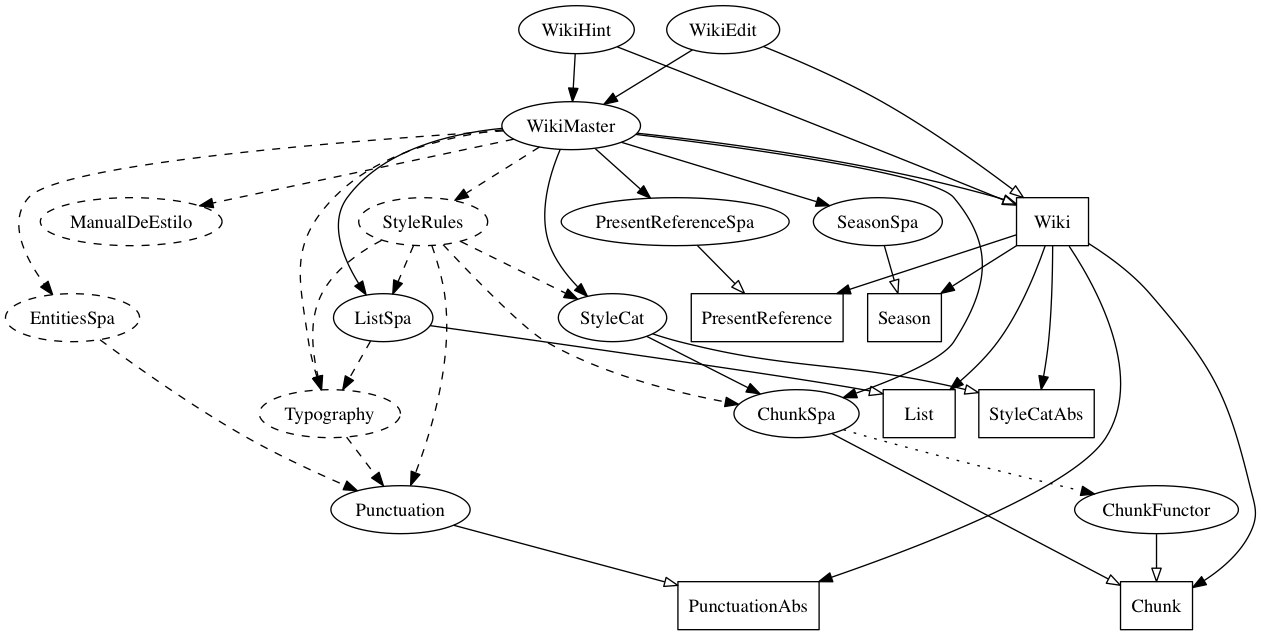
\includegraphics[width=\textwidth]{img/grammar/grammar_full}
\caption{Full module structure and dependencies that make up StyleCheck}
\label{fig:grammar_full}
\end{figure}

\graffito{Code for the three main modules \texttt{Wiki}, \texttt{WikiMaster} and \texttt{WikiHint} can be found in \autoref{app:code}}
First, we will describe the main grammar components. This subset of the full grammar is shown in \autoref{fig:grammar_simple}. The main abstract syntax module is \texttt{Wiki}, which contains a function for each of the rules (\autoref{lst:wiki}). This abstract syntax has three corresponding concrete syntax modules: \texttt{WikiMaster}, \texttt{WikiHint} and \texttt{WikiEdit}. \texttt{WikiMaster} (\autoref{lst:wikimaster}) contains the main parsing mechanics. In it, each abstract syntax function is linearised into the required type: \texttt{StyleRule}, \texttt{StyleHint} or \texttt{StyleLookup}:

\begin{figure}[h]
\myfloatalign
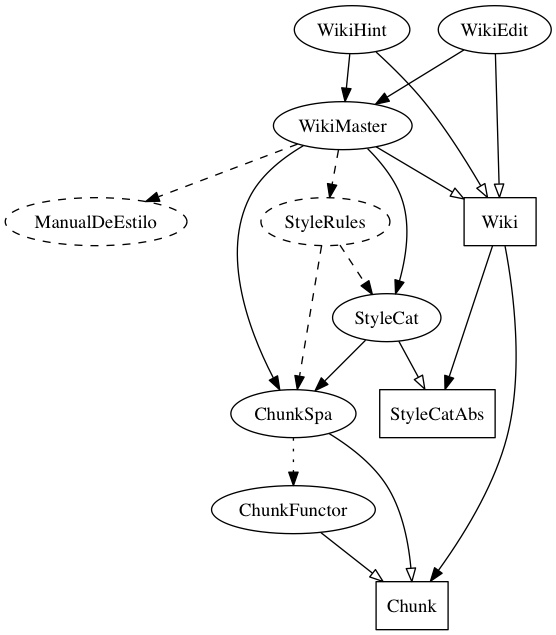
\includegraphics[width=0.8\textwidth]{img/grammar/grammar_simple}
\caption{Main StyleCheck modules and dependencies}
\label{fig:grammar_simple}
\end{figure}

\begin{itemize}
    \item These three types are defined in the abstract syntax \texttt{StyleCatAbs} and in the concrete \texttt{StyleCat}. 
    \item Convenience functions to build these types are provided in the resource module \texttt{StyleRules}.
    \item To build the options, \texttt{WikiMaster} uses the necessary components from the Spanish \spacedlowsmallcaps{RGL} (not shown in \autoref{fig:grammar_simple}). 
    \item The text for the style hints is contained in \texttt{ManualDeEstilo}.
\end{itemize}

\noindent Once the required style types are built, \texttt{WikiMaster} builds \texttt{Chunk} types out of them. The idea is that when parsing a sentence, once or more \texttt{Chunk}s (each corresponding to a style rule, hint or lookup) are identified, appended together, and output as the result of the parse. To acheive this, StyleCheck makes use of the chunking types and functions used in the Wide-Coverage Translator being built upon \ac{GF} \parencite{ranta2014embedded}. The abstract syntax for these types is \texttt{Chunk}, and the concrete is \texttt{ChunkSpa}. Finally, the top level type, a \texttt{Phr}, is built out of one or more \texttt{Chunk}s.

To sum up, the parsing mechanics are as follows:

\begin{enumerate}
    \item A style rule is matched and a style rule, hint or lookup type is built.
    \item \texttt{WikiMaster} selects the \texttt{options} from the style record and builds a \texttt{Chunk} out of them.
    \item Through the functions included in \texttt{ChunkSpa}, a \texttt{Phr} type is built, which is the top level category in the grammar.
    \item The tree constructed until now is linearised using \texttt{WikiHint}. This concrete syntax selects the \texttt{hint} field from the style type record, resulting in the hint text being output.
    \item A simple regex extracts all the hints from the output (hints are delimited with \texttt{|||} to make this task easy). Any non-matches will simply return the original token.
\end{enumerate}

The additional modules shown in \autoref{fig:grammar_full}, such as \texttt{ListSpa} or \texttt{Typography} ease the task of writing style rules. They mainly contain functions and opers related to a specific rule in StyleCheck.

Finally, there is one extra concrete syntax that isn't used in this thesis. The \texttt{WikiEdit} shows how an automatic post-editing tool would work. It simply selects the \texttt{approved} field from the style record instead of the hint for \texttt{StyleRule}s (the only types that have an approved field). This kind of funtionality for \ac{CAT} tools needs further thought and development, since it could be very confusing for translators to find parts of their texts changed without warning.

\section{Intrinsic evaluation}

\noindent In order to develop the grammar, the possible options for each rule had to be thought out. A test sentence was created for each option, together forming a small corpus. The grammar was developed so that it would generate the correct output on the small corpus of options. This was evaluated by having \ac{GF} parse the sentences and check that the grammar brings up the correct style hint.

Intrinsic evaluation as described will perform well on the corpus, but some cases can fall through the net. Looking into the final translations carried out by the experiment's participants, two cases were found of options that the grammar did not detect:

\begin{itemize}
    \item Rule 2.B (\autoref{lst:wiki}, \autoref{lst:wikimaster}) states that temporal references should not use the moment of enunciation as reference point. For example, in ``Her most recent work'', \textit{recent} refers to the moment of enunciation. Future readers may consider \textit{recent} as a different time period than the writer, so it should be avoided. Even though StyleCheck was developed with several adverbial time markers that refer to the moment of enunciation (\textit{recientemente}, \textit{hoy}, \textit{ahora}, etc.), one participant used an adjective form instead (``la más reciente''), which was not in the grammar and did not generate a hint.
    \item Another simpler case is that of the \spacedlowsmallcaps{USA}. The acceptable forms in Spanish are \spacedlowsmallcaps{EE. UU.} (with a space) or \spacedlowsmallcaps{EUA}. Several non-approved options were generated, such as \spacedlowsmallcaps{EE.UU.} (without a space) or \spacedlowsmallcaps{USA}. One participant, however, used the form \spacedlowsmallcaps{EEUU}, which was not in the grammar and would not have triggered a style hint.
\end{itemize}

The advantage of having built a prototype is once again clear. The previous issues can be solved straight away and directly integrated into a future version of StyleCheck.
 % Chapter 7
% Chapter X

\chapter{Experiment Website} % Chapter title
\label{ch:website} % For referencing the chapter elsewhere, use \autoref{ch:name} 

%----------------------------------------------------------------------------------------
\section{Experiment Walkthrough}
\label{sec:walkthrough}

\noindent A detailed walkthough of the experiments with screenshots is presented in \autoref{an:walkthrough}. The following subsections provide a more detailed description of the technical side of the server setup (\autoref{sec:server_setup}), how participants found out about the experiment (\autoref{sec:access}), the StyleCheck user interface (\autoref{sec:hint_ui}) and the data that was logged (\autoref{sec:logging}).

%----------------------------------------------------------------------------------------

\section{Server Setup}
\label{sec:server_setup}

\noindent The website where participants carried out the translation tasks was created specifically for this experiment. The website was built using the Flask\footnote{\url{http://flask.pocoo.org/}} (v. 10.1) web framework and Python (3.4.3) from a virtual environment to help manage package dependencies. The \texttt{html} and \texttt{css} code was put together using Bootstrap\footnote{\url{http://getbootstrap.com/}}. The dynamic parts of the user interface were written in \texttt{javascript} using the jQuery\footnote{\url{http://jquery.com/}} library. Using these frameworks, the website was responsive and thus able to be used on mobile devices, although not recommended for this experiment. Despite this recommendation, one participant reported carrying out the experiment on an iPad.

The server ran Ubuntu 12.04 and was set up with nginx\footnote{\url{http://nginx.org/}} (v. 1.9.0) as the front-end reverse proxy and uWSGI\footnote{\url{https://github.com/unbit/uwsgi}} (v. 2.0.10) as the application server communicating with Flask through the \spacedlowsmallcaps{WSGI} protocol\footnote{\url{https://www.python.org/dev/peps/pep-3333/}}. The server had 16 \spacedlowsmallcaps{GB} of \spacedlowsmallcaps{RAM}, 8 \spacedlowsmallcaps{CPU}s and 40 \spacedlowsmallcaps{GB} of \spacedlowsmallcaps{SSD} disk.

\graffito{Note: Due to the embedding of the Google survey form, a large blank space appears in \autoref{fig:web_initial}. Please see \autoref{sec:server_setup} for further explanation.}
The questionnaires were made using Google Forms\footnote{\url{https://www.google.com/forms/about/}} and the results downloaded and analysed as \texttt{.csv} files. Forms created with Google Forms can either be answered by following a link or they can be embedded into a website. For this experiment, the latter option was chosen so as to be less jarring for participants. However, forms can only be embedded into an \mintinline{html}|<iframe>| element. Since some questionnaire pages contained more questions than others, some pages included a lot of blank space in the \mintinline{html}|<iframe>| (see \autoref{fig:web_initial}) while others with more questions had to be scrolled.

%----------------------------------------------------------------------------------------

\section{Experiment Access}
\label{sec:access}

\noindent To access the experiment, participants were requested to contact an email address provided in the Call for Participation announcement. Then, they were provided with a unique link from which to access the experiment. The link \spacedlowsmallcaps{URL} included a unique Participant \spacedlowsmallcaps{ID}, which identified the participant throughout the experiment, and a unique text-setup combination. This enabled the experiment to be carried out with all the possible number of combinations for texts and setups. For example, the \spacedlowsmallcaps{URL} \texttt{www.dvh.io/main/420/123} indicates that the Participant \spacedlowsmallcaps{ID} is 420, Text 1 should be used in the \scratch setup, Text 2 in the \ac{PE} setup and Text 3 in the \style setup.

%----------------------------------------------------------------------------------------

\section{StyleCheck User Interface}
\label{sec:hint_ui}

\noindent The third setup interacted dynamically with the server to show participants style hints as they translated. Every time a \mintinline{html}|<textarea>| where translations where input lost focus, the contents were sent to the server, analysed using StyleCheck, and any style rules parsed sent to the participant's browser. Before sending them, the hints were checked for duplicates (some hints could be generated multiple times in a parse) and if any were found only one instance of the rule was returned. The rules then showed up in a red panel below the corresponding sentence that was parsed (\autoref{fig:hints}).

\begin{figure}[h]
\myfloatalign
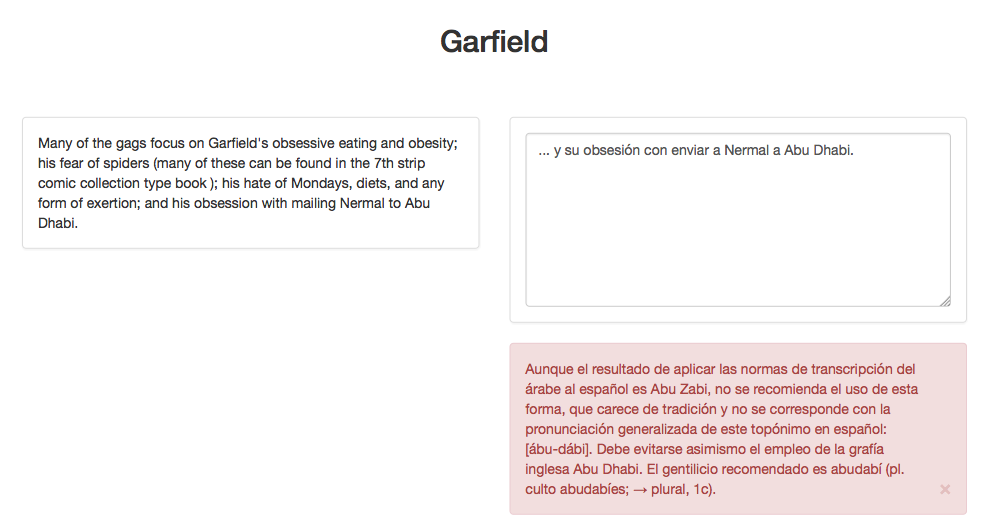
\includegraphics[width=\textwidth]{img/hints/hints.png}
\caption{Hints being shown to the participants after analysing their translations with StyleCheck.}
\label{fig:hints}
\end{figure}

In some cases, due to the length and number of the hints, the panels could take up a lot of space.  Depending on the size of the participant's display and the size of the browser window, the hints could even be rendered outside the visible part of the screen, requiring participants to scroll (\autoref{fig:hints_long}).

\begin{figure}[!ht]
\myfloatalign
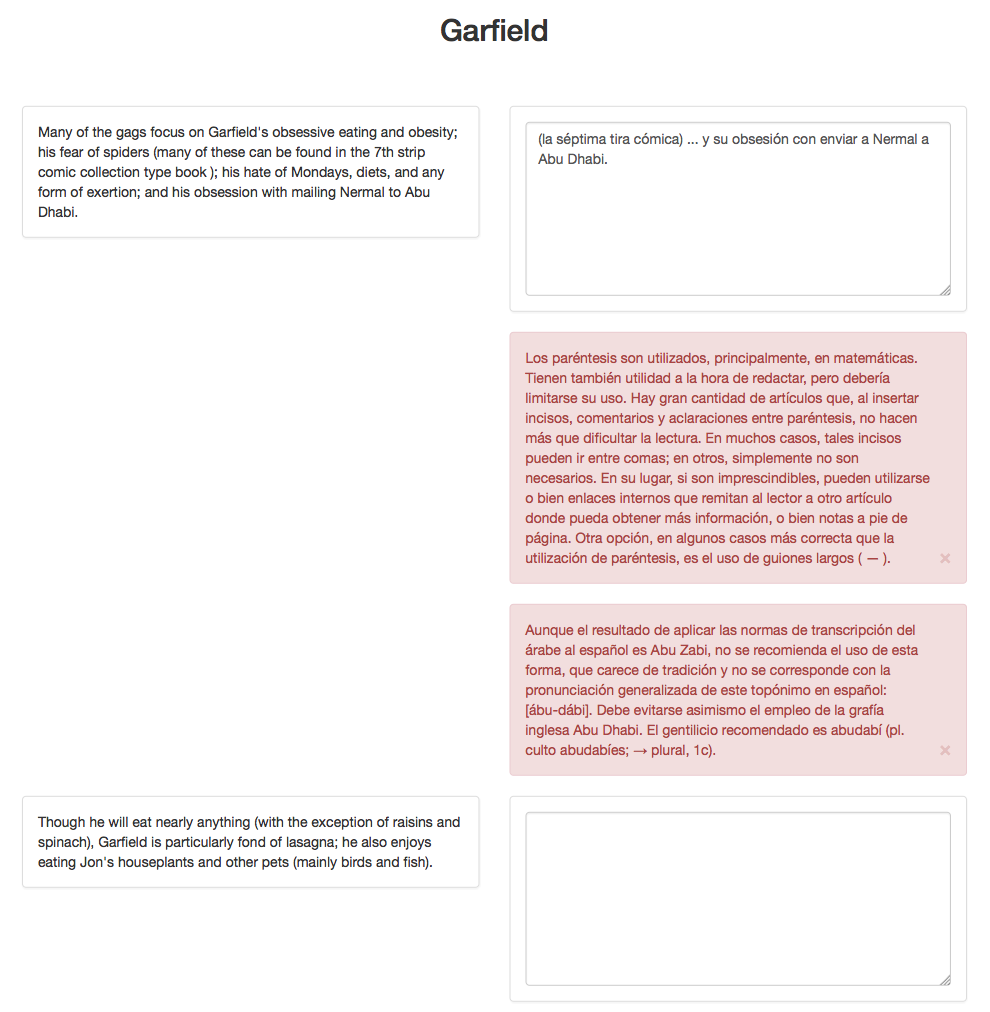
\includegraphics[width=\textwidth]{img/hints/hints_long.png}
\caption{Two long hints being shown taking up a large part of the screen.}
\label{fig:hints_long}
\end{figure}

%------------------------------------------------

\section{Logging}
\label{sec:logging}

\noindent Different kinds of logging, in addition to saving the final translations, were set up in the server:

\begin{itemize}
\item \textit{Style guide click}: When a participant clicked on the link to Wikipedia's style guide, the page the participant was on (the translation brief is shown on four different pages, see \autoref{an:walkthrough}) and the click time was registered.
\item \textit{Translation information}: The website saved the actual translation, as well as the start and end time for each setup.
%\item \textit{Key activity logging}: The website recorded when a key was pressed within the \mintinline{html}|<textarea>| elements where participants wrote in their translations. Both the time and key was recorded. Due to a lack of time, key activity for special keys (backspace, shift, etc.) were not able to be recorded, although the moment when one was pressed was logged. Thus, the logged data should only be considered useful to track key-press activity and not the actual keys themselves.
\item \textit{Hints}: For the \style setup, the contents of the \mintinline{html}|<textarea>| element, the time and any style hints returned were logged.
\end{itemize}


%----------------------------------------------------------------------------------------

 % Chapter 8
% Chapter 8

\chapter{Questionnaires} % Chapter title
\label{ch:questionnaires} % For referencing the chapter elsewhere, use \autoref{ch:name} 

%----------------------------------------------------------------------------------------

\graffito{Note: For screenshots of the actual questionnaire, please see \autoref{an:questionnaires}.}

\noindent For this study, two questionnaires were created. The initial questionnaire was completed by participants before carrying out the translation tasks, while the final questionnaire was filled in after.

The questionnaires contained both open and closed questions. An overview of the questions and the research objectives each one aimed to cover are provided in the following subsections. Each question is given a number, although the actual questionnaire did not number the questions so that it didn't seem too long to participants. For this same reason, each questionnaire was presented split into pages and a progress bar shown at the bottom of each page. Options for the closed questions were randomly shuffled. 

Given that the majority of participants were likely to be native Spanish speakers and non-native English speakers, the questions were written in English but participants could answer the longer questions in either Spanish or English. Since they would be translating from English, a certain level of knowledge of English was presupposed and it wasn't deemed necessary to offer the questions also in Spanish.


%------------------------------------------------

\section{Initial Questionnaire}

\noindent This questionnaire gathered basic demographic data on the participants, as well as their previous experience with translation and various translation-related tasks. It was also exploratory in nature in that it tried to discover what tasks translators would like to be automated, as well as their opinions on \ac{MT} and it's relation to \ac{CAT}.

The specific research aims for the initial questionnaire and the questions related to them are the following:

\graffito{Note: numbers in brackets refer to the specific questions in the initial questionnaire. Please see \autoref{an:questionnaires} for the full questions.}
\begin{itemize}
\item Basic participant demographics (age, gender, occupation, languages) [Questions 2, 3, 4, 5, 6]
\item Participant's experience and training as translators [Questions 7, 8, 9, 10]
\item Participant's experience with specific translation-related tasks [Question 11]
\item Participant's experience with specific translation-related tools [Questions 18, 19, 20]
\item What do translators themselves consider translation to be? [Questions 1, 15, 16, 17]
\item What are the most important considerations when translating? [Questions 15, 16, 17]
\item What tasks carried out during translation are candidates for automation? [Questions 12, 13, 14]
\item What attitudes do translators have towards machine translation? [Questions 21, 22, 23]
\end{itemize}

%------------------------------------------------

\section{Final Questionnaire}

\noindent The final questionnaire asked translators to compare the three translation tasks performed and asked specific details about each individual task. Following \textcite{krings2005wege}, this questionnaire can be categorised as a retrospective questionnaire (related to a specific task) and as online (the researcher was not present while the questions were answered). 

\textcite{christensen2011studies} notes that a downside to retrospective questionnaires is the risk that subjects might make up explanations since they have to retrieve information from long-term memory. This study tried to partially offset this concern by providing participants with the full \ac{ST} (and \ac{MT} suggestion for the second task) directly above the final questionnaire, so that they could more easily remember the texts and answer the questions (see \autoref{fig:web_final}). The participant's own translations were not provided so that they would not get frustrated at seeing any possible mistakes they had made. 

The specific research aims for the final questionnaire and the questions related to them are described in the following list:

\graffito{Note: numbers in brackets refer to the specific questions in the final questionnaire. Please see \autoref{an:questionnaires} for the full questions.}
\begin{itemize}
\item Which setup was preferred by the translators? [Questions 14, 15, 22, 23, 32, 33]
\item Which factors made a text easy or difficult to translate? [Question 3, 4, 5, 6]
\item Which setup helped translators produce a better translation (perceived or real)? [Question 15, 23, 33]
\item Did they perceive any differences regarding how in control they were of their own final translations between the setups? [Questions 7, 8, 9, 10]
\item Did their perceived translation speed vary significantly from their real translation speed? [Questions 11, 17, 25]
\item Were the style hints useful for participants? [Question 28, 29, 30, 31, 32, 33]
\item Did participants find the \ac{MT} suggestions useful? [Question 20, 21, 22]
\end{itemize}

Some of the questions were exploratory in nature and could be categorised into various of the previous aims depending on the participant's answer. Very general and open questions were asked to encourage participants to come up with their own ideas about the three setups. Mainly, these questions were 3, 4, 5, 6, 12, 13, 16, 18, 19, 24, 26, 27, 34 and 35.

Questions 14, 20, 22 and 32 followed those used by \textcite{carl2015post}. The wording was slightly adapted to fit in with the current study. The question ``Overall, how satisfied were you with the task of translating Text X?'' (questions 14, 22 and 23) was complemented with ``Overall, how satisfied were you with the quality of your final translation of Text X'' (questions 15, 23 and 33) to separate the performance of the actual task from its output. The single question offered by \textcite{carl2015post} could be ambiguous and make participants hesitate between liking the task but not being satisfied with its final result.

A possibility that was considered was to include the System Usability Scale (\spacedlowsmallcaps{SUS}) \parencite{brooke1996sus} questions into the final questionnaire. The \spacedlowsmallcaps{SUS} is a widely-used set of 10 questions that measure the usability of a system. Despite the advantages of using a well-known questionnaire, it was decided to not include them. The 10 questions would have had to be provided for each of the three setups to allow for comparison. An extra 30 questions added to the final questionnaire was deemed to make it too long and fatiguing for participants.


 % Chapter 9

%------------------------------------------------

\ctparttext{} % Text on the Part 4 page describing the content in Part 4
\part{Results} % Fourth part of the thesis


% Chapter 10

\chapter{Results and Discussion} % Chapter title
\label{ch:results}

%----------------------------------------------------------------------------------------

\section{Participant Demographics}

\graffito{Questions are prefixed with a letter indicating which questionnaire they appear in (\textit{I} for initial and \textit{F} for final) followed by the question number. For a detailed look at the questions, please refer to \autoref{an:questionnaires}.}

\noindent A total of 11 participants answered the Call for Participation (see \autoref{sec:online}) and requested a participation link. Of those, one did not attempt to complete the experiment. One further participant completed all experiment parts except filling in the initial questionnaire, so the provided results were not used. Thus, in total 9 participants completed the experiment, which represents 82\,\% of people who requested to participate. Given that one participant mostly completed the experiment and a technical issue may have caused the initial questionnaire not to be saved, that brings the participation rate up to 91\,\%. These figures suggest the approach of asking interested people to request a link and implicitly commit to carrying out the experiment (see \autoref{sec:online}) was effective.

Genderwise, 4 male (44\,\%) and 5 female (56\,\%) participants took part, all in the 20-25 age group. All participants considered themselves native Catalan speakers, while all but one (89\,\%) considered themselves native Spanish speakers (the odd one out did select Spanish as one of the languages he or she speaks). Other languages spoken by the participants include English (100\,\%), French (78\,\%), Spanish (33\,\%), Japanese (22\,\%), German (11\,\%), Italian (11\,\%), Korean (11\,\%), Dutch (11\,\%), Polish (11\,\%) and Catalan (11\,\%). As well as the aforementioned participant, the Spanish and Catalan results are due to a participant selecting them in both the native languages and other languages questions.

All participants have studied translation, during either 4 years (67\,\%) or 5 years (33\,\%) [Question I.9]. Regarding professional experience as translators, 56\,\% reported having worked as translators, while 44\,\% hadn't. Of those that had, 40\,\% had worked for 2 years as a translator, 40\,\% for 1 year and 20\,\% for less than 1 year [Question I.10].

When asked specifically about their professional experience [Question I.11], 56\,\% reported having translated from scratch; 44\,\% reported experience with proof-reading, \ac{PE} and localising; 22\,\% said terminology management, using \ac{CAT} tools and preparing documents for internationalisation; and 11\,\% mentioned transcreation, setting up style guides, \ac{MT} quality evaluation and subtitling. It is interesting to note that the answers to Question 11 and the previous Questions 9 and 10 don't match up as expected, \ie some participants who reported not having worked as translators then went on to say they had professional experience translating from scratch, for example. It is possible that in interpreting the question, participants included internships and odd jobs which they did not fully consider to be ``work''.

Given the previous descriptions, the participants can be classified as semi-professionals: they are no longer students, but still not as experienced as a long-standing professional.


%----------------------------------------------------------------------------------------

\section{Conceptions of Translation}

\noindent This section describes what the participants think about translation [Questions I.1 and I.12--I.23]. The aim of these questions is two-fold. On the one hand, they aim to provide more context for the tool evaluations the participants provide. On the other hand, they aim to verify if translators are a useful source of suggestions of how to improve \ac{CAT} tools.

\subsection{Translation Tasks}

\noindent Participants were asked which tasks they considered boring and which they considered interesting. It is assumed that the boring tasks would be those that a translator would prefer not to do and thus could be considered as a candidate for automation. 

Participants considered that researching and learning about a new topic is one of the most interesting tasks in translation, as well as the process of translation itself [Question I.12]. The problem solving aspect was also frequently mentioned, such as solving cultural clashes and difficulties present in the text. Creativity also came up, a topic which can surprise those who consider translation to be an essentially mechanical task but which is frequently discussed in translation theory. As for what participants found boring when translating [Question I.13], 33\,\% also mentioned topic research. Other aspects considered boring were revising and proofreading, page layout management, terminology research and database management (I interpret this as glossary and translation memory management). One participant even explicitly mentioned \ac{PE} as a boring task.

The questionnaire asked participants that if they could have a tool to automate any task in translation, which task would it be [Question I.14]. A few mentioned the same tasks they considered boring, such as topic research and proofreading. Interestingly, many of the tools they wished for were those that provide suggestions of various kinds: collocations and expressions, synonyms, translation options in context and problematic structures in the text. This suggests participants wished to remain in control of their translations and have the power to pick an option, rather than being forced an option in the case of \ac{TM} and \ac{PE} which they then have to change only if necessary (as most \ac{PE} guidelines state, see for example \textcite{carl2015post}). 

Thus, it appears that simple questionnaires asking translators what tasks they would like to be automated is a useful way to come up with \ac{CAT} tool improvements. It also shows that not all improvements can please everyone: one participant stated they had all the tools they needed to translate while another explicitely mentioned \ac{PE} as an activity they dislike.


\subsection{What Makes a Good Translation}

\noindent The question of translation evaluation ---what a good and a bad translation is, if they can even be classified as such--- is inextricably linked to how translation is conceptualised. Participants were asked what translation meant to them [Question I.1]. To analyse the responses, the translation theory paradigms discussed in \autoref{sec:paradigms} provide a good starting point. Given the freeform answers and open-ended question, it is difficult to classify a participant's views in one paradigm or the other. However, a large number of responses describe translation in a similar fashion to the equivalence paradigm, some nuancing this description with tints of functional priorities and the need to adapt the text to the target culture and function. 

To garner a more detailed and nuanced view, participants were asked to rate specific considerations on a scale of 1 to 5, where 1 is very important and 5 is not at all important [Question I.15]. As can be seen in \autoref{tab:considerations}, all considerations were important to the participants. Grammaticality of the final product was the most important priority, followed by conforming to client requirements. Interestingly, accurately portraying the \ac{ST} was second to last in the ranking, only more important than applying a style guide. These results seem to indicate that despite their initial answers, participants view translation in line with the skopos/functional paradigm.

\begin{table}[h]
\myfloatalign
\begin{tabularx}{\textwidth}{Xcc} \toprule
\tableheadline{Consideration} & \tableheadline{Mean rating} & \tableheadline{\sigma} \\
\midrule
Providing a grammatically correct translation & $1.2$ &  $0.44$ \\
Conforming to what the client requests in the translation brief & $1.4$ & $0.53$ \\
Providing a fluent translation/idiomatic translation & $1.6$ & $0.73$ \\
Using terminology consistently & $2.0$ & $1.12$ \\
Accurately portraying the source text & $2.1$ & $0.78$ \\
Applying a style guide consistently & $2.2$ & $1.20$ \\
\bottomrule
\end{tabularx}
\caption{Mean ratings and standard deviation for the importance of various considerations when translating, with 1 being very important and 5 being not at all important.}  
\label{tab:considerations}
\end{table}

When asked which of the considerations they prioritised the most [Question I.16], 56\,\% indicated providing a fluent/idiomatic translation, followed by providing a grammatically correct translation and accurately portraying the \ac{ST} with 22\,\% each. Once again, even though the \ac{ST} is important, \ac{TT} considerations are generally more important. Regarding other considerations [Question I.17], one participant mentioned varying his or her priorities depending on the \ac{TT} function.


\subsection{Tools and Resources}

\noindent Regarding what tools the participants normally use, 78\,\% reported using both glossaries and style guides. \ac{CAT} tool usage was lower, only 57\,\% stated they regularly use them when translating.

Another interesting aspect were participants' views on \ac{MT}. The majority of participants were uncertain about its usefulness to translators (67\,\%), with the rest saying it was useful. Similar views were gathered when asked if \ac{MT} is only useful for the general public: 44\,\% remained neutral, while a third of them disagreed. This could indicate that some of those hesitant to say \ac{MT} is useful for translators conceded that it does have professional use beyond gisting systems.

The majority of participants did not think \ac{MT} will replace translators (78\,\%), the rest being uncertain about it. This could be related to their perceptions of \ac{MT} quality, as 67\,\% considered that it does not provide good quality translations today, with 33\,\% being unsure. The uncertain responses could indicate that the translators are out of touch with current \ac{MT} research and how \ac{MT} systems work: 44\,\% stated it's difficult to understand how \ac{MT} works and the rest were devided between being unsure (22\,\%) and saying it is easy to understand (33\,\%). A large majority (78\,\%) did state their willingness to learn more about \ac{MT}.

Finally, all participants considered their translations are better than those provided by \ac{MT}. When asked why, they responded in a more nuanced way. As one participant put it, ``anything beyond grammar and vocabulary is lost''. Many mention its lack of adaptability to client and target culture requirements, it can't deal with humour and cultural clashes, etc. In essence, it lacks the ``human factor'' as some participants put it. This makes the translations ``very standardised'' and doesn't take style into account. Despite all the downsides, one participant did concede that the results are good enough and fast for certain language pairs.


%----------------------------------------------------------------------------------------

\section{Time and Speed}

\noindent Time is one of the preferred metrics for evaluating \ac{PE}. A large number of studies present it in the form of speed defined as $words/hour$ \parencite{federico2012measuring}, although others use $seconds/word$ \parencite{koponen2012post}. For this thesis, $words/hour$ was chosen. Two forms of time data were collected: real time spent on each translation by way of logging on the server app and the time translators perceived they spent on each translation by way of the final questionnaire [Questions F.11, F.17 and F.25]. The results were converted to $words/hour$ and analysed.

It is also worth noting that this study considers the total translation time for each text from opening the document to saving the final translation. This time could include Internet searches, glossary and other linguistic resource lookup, a quick glance at a phone, a sip of coffee, etc. This is in contrast to the approach taken by \textcite{federico2012measuring}: they only consider segments where the translator is actually ``translating''. They determine this by setting a processing threshold for the segments included in their analysis (between 30 and 0.5 $seconds/word$) and discard the rest. This threshold ignores many of the tasks a translator carries out and which should be considered part of the translation process, such as terminology lookup and topic documentation. It can often be the case that searching for a single term can take longer than ``translating'' the rest of the text. Even though the authors specify that their choice of speed as an evaluation metric is intended to correlate with translation cost, the thresholds they set ignore the tasks carried out during translation which can be the most costly in terms of time.

\subsection{Setups and Texts}

\noindent Both text and setup have an effect on the translation speed. \autoref{fig:time_real_setup} shows that \ac{PE} is the fastest setup to translate in, with \scratch and \style performing similarly. \autoref{fig:time_real_text} shows that text also plays an important role: \garfield achieves the highest average speed across all setups, followed by \ai and then \charlotte. This lines up with how much participants liked to translate a certain text and how hard they thought it was (this data is detailed in \autoref{sec:setup_prefs}). Digging further into the data, \autoref{fig:time_real_ts} shows that the fastest combination by far is \garfield in the \ac{PE} setup. \scratch shows speed variance among texts, while \style evens out the speed differences.

\begin{figure}[h]
\myfloatalign
\subfloat[Setup]{
\label{fig:time_real_setup}
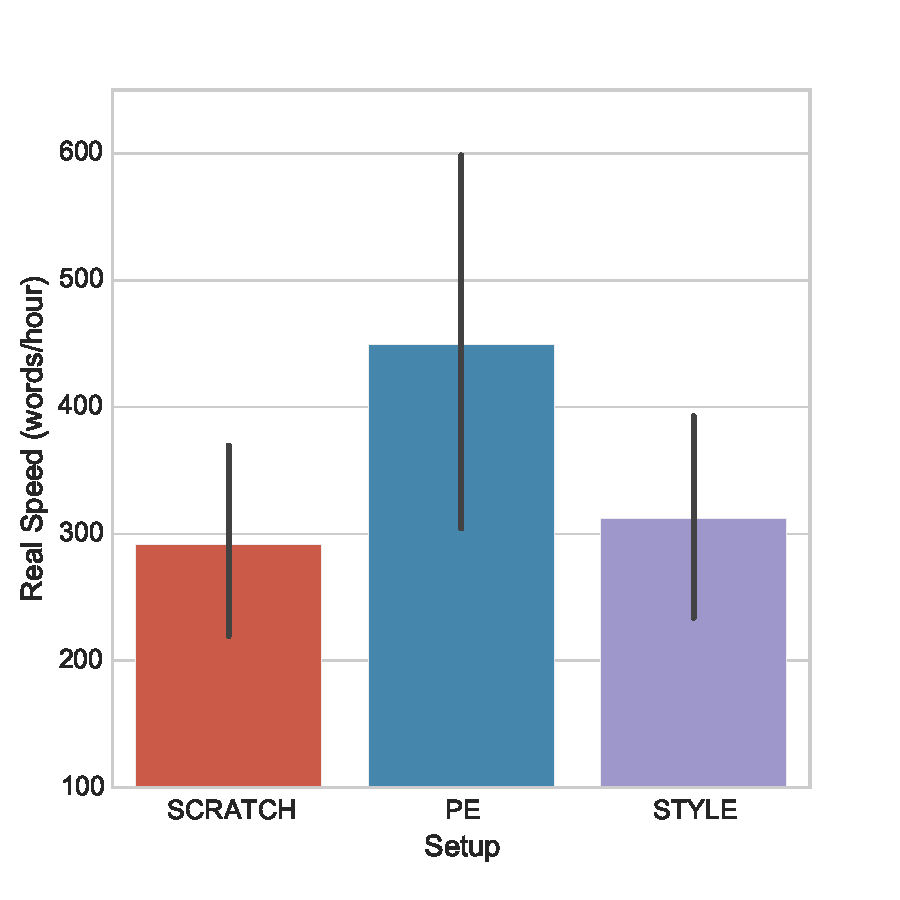
\includegraphics[width=0.45\textwidth]{img/time/time_real_setup}}
\subfloat[Text]{
\label{fig:time_real_text}
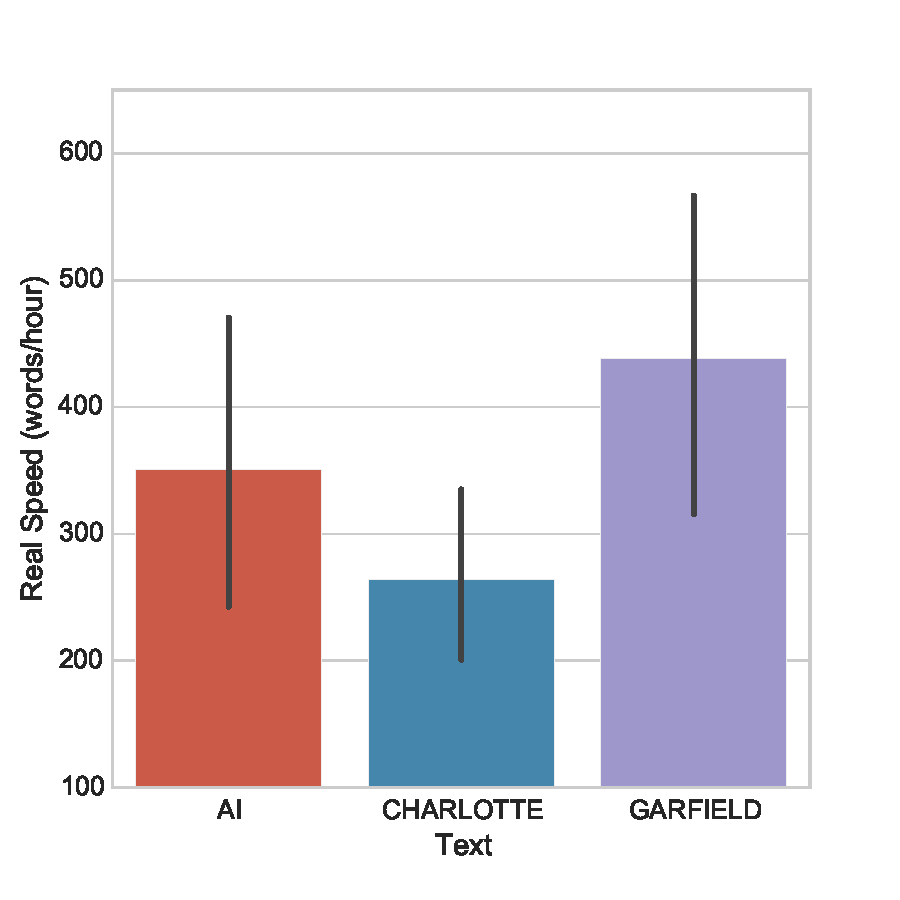
\includegraphics[width=0.45\textwidth]{img/time/time_real_text}}
\caption{Mean speeds per setup and per text. 95\,\% confidence interval calculated using bootstrap resampling.}
\label{fig:time_real_vs}
\end{figure}

\begin{figure}[h]
\myfloatalign
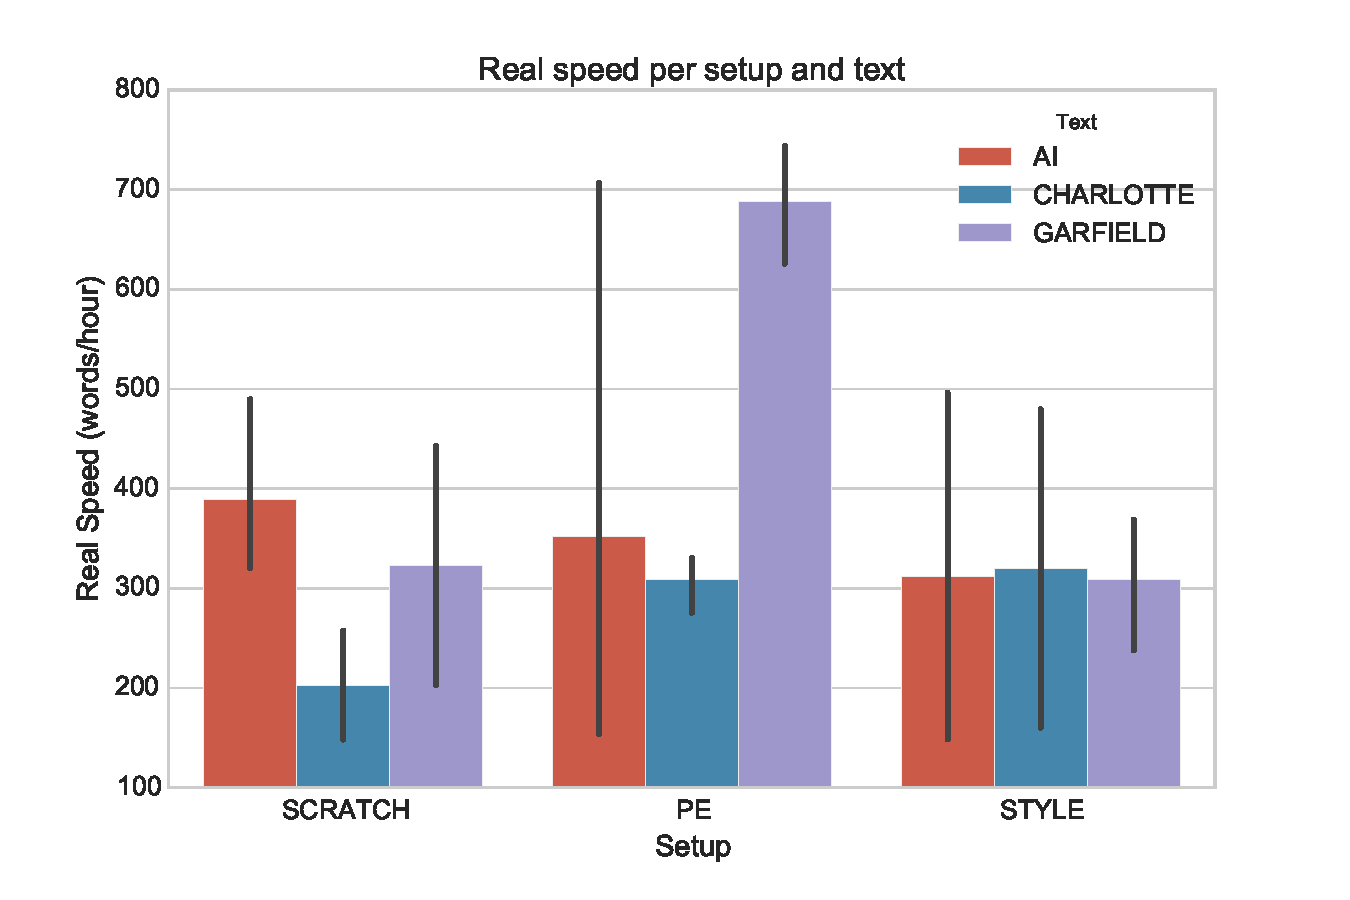
\includegraphics[width=0.8\textwidth]{img/time/time_real_ts}
\caption{Mean speeds broken down per setup and per text. 95\,\% confidence interval calculated using bootstrap resampling.}
\label{fig:time_real_ts}
\end{figure}

\subsection{Participants}

\noindent Individual variation is a strong factor in speed considerations. As can be seen in \autoref{fig:time_box_participant} and \autoref{fig:time_speed_participant}, speeds can range between just over 100 to over 700 $words/hour$ depending on the translator and the setup. Some participants such as 421, 423, 425 and 427 translate at a fairly constant speed across texts and setups. Others, such as 424 and 429, experience major speed differences across setups. In particular, \autoref{fig:time_speed_participant} shows these latter two participants experience a major speed-up in the \ac{PE} setup, which could indicate they only minimally edited the \ac{MT} output. To confirm this, \spacedlowsmallcaps{BLEU} \parencite{papineni2001bleu} scores were calculated between the \ac{MT} suggestions and the final post-edited translations. \spacedlowsmallcaps{BLEU} is usually used to score how well a machine-translated text matches a reference translation, here the metric is used to see how much editing was performed on the \ac{MT} suggestions by the participants. \autoref{fig:time_real_bleu} shows a correlation (Pearson's $r = 0.75$) between the \spacedlowsmallcaps{BLEU} scores and the time spent post-editing. This correlation is also present in the time participants thought they had spent on the task (\autoref{fig:time_perceived_bleu}, Pearson's $r = 0.8$).

\begin{figure}
    \myfloatalign
    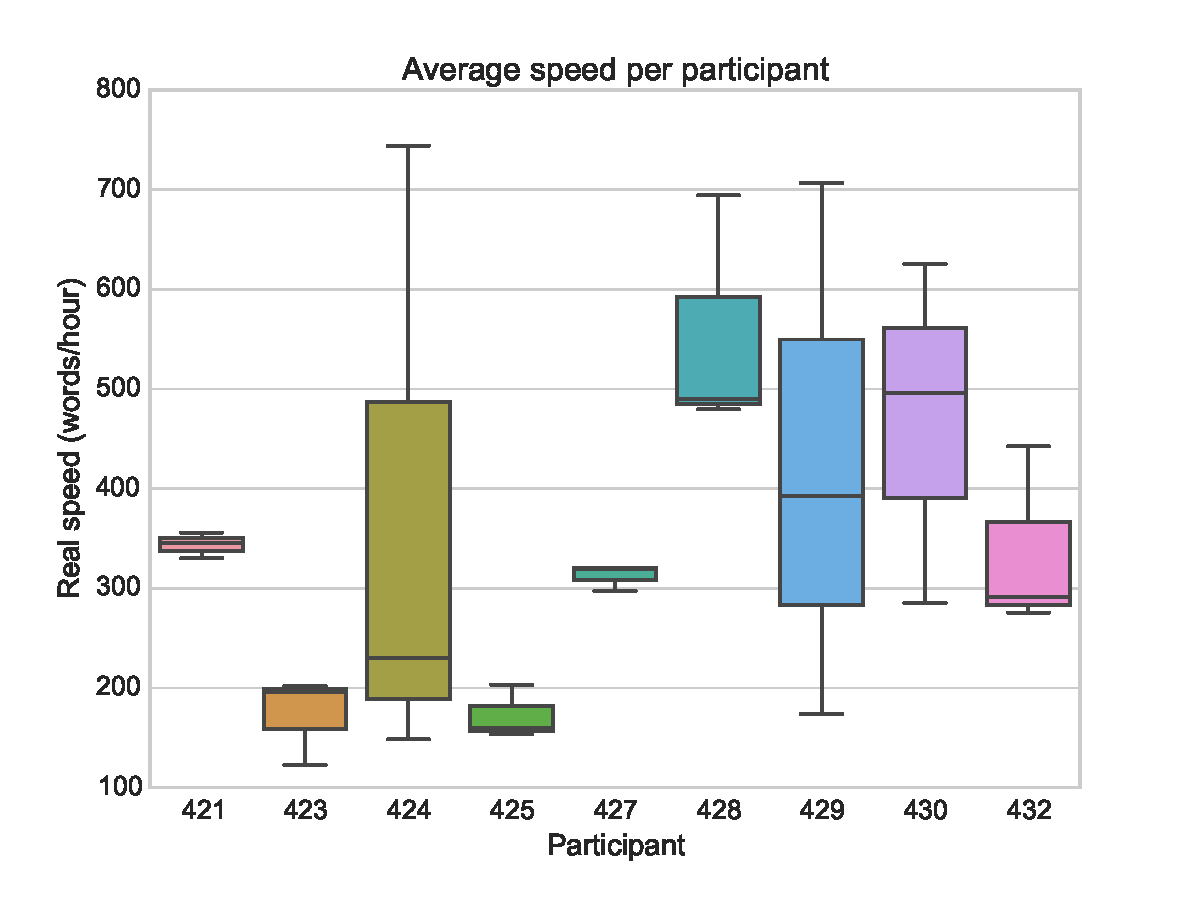
\includegraphics[width=0.8\textwidth]{img/time/time_box_participant}
    \caption{Mean real speeds per participant}
    \label{fig:time_box_participant}
\end{figure}

\begin{figure}
    \myfloatalign
    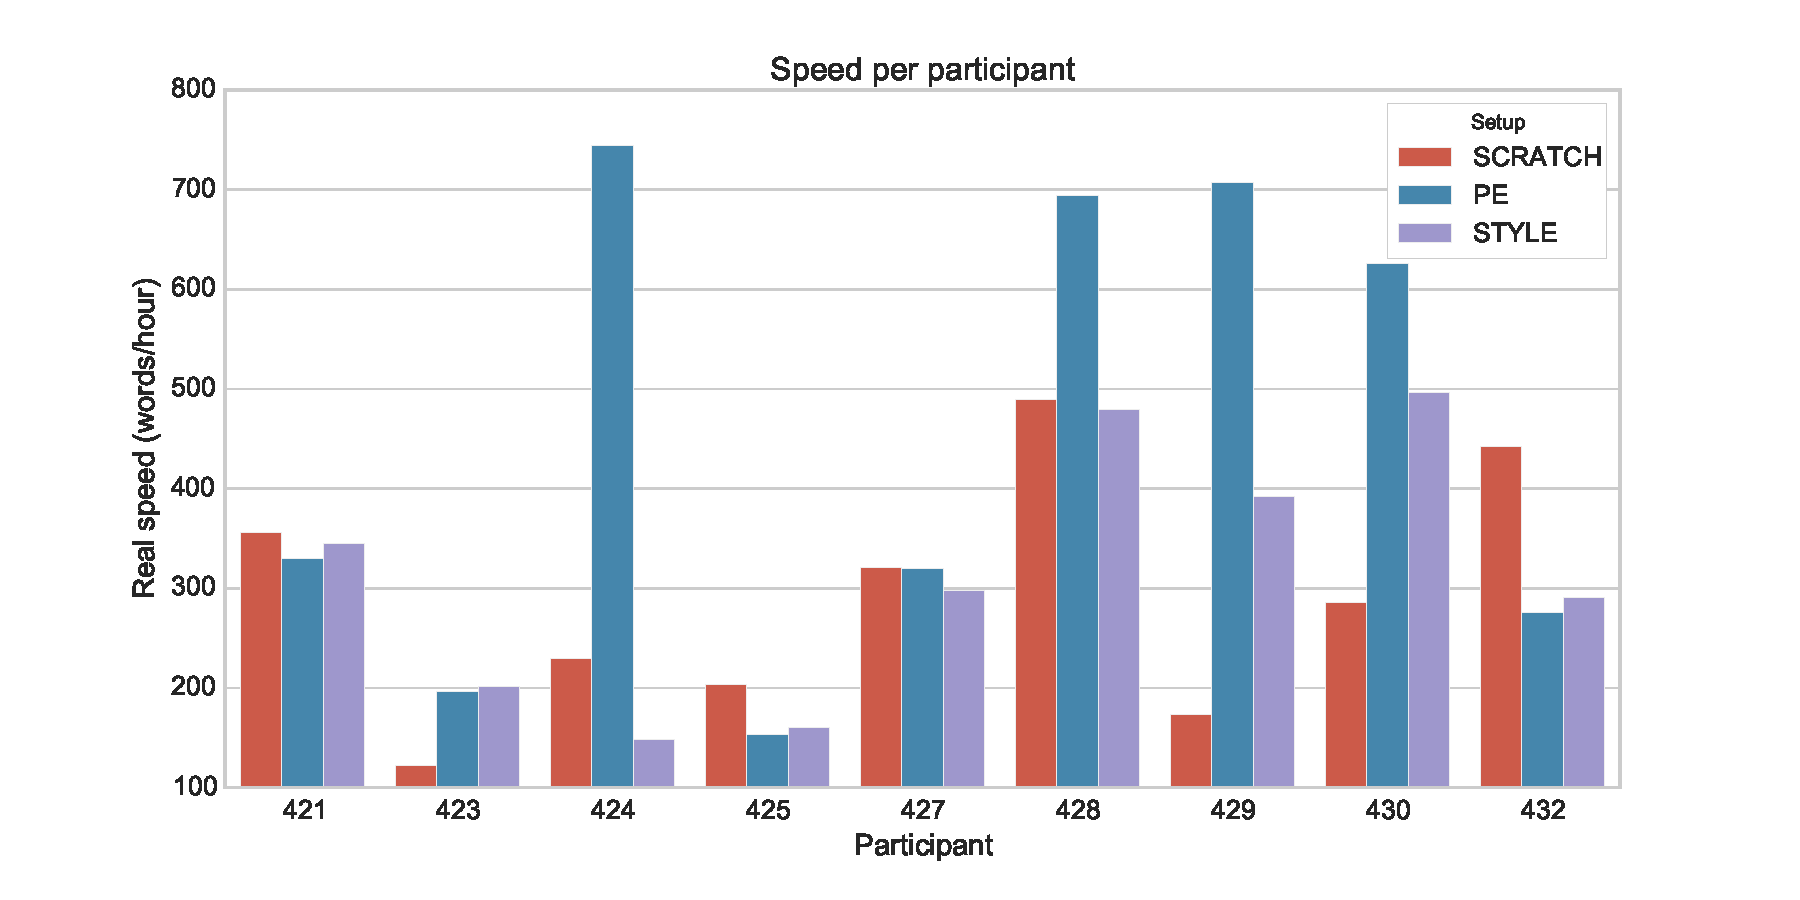
\includegraphics[width=\textwidth]{img/time/time_speed_participant}
    \caption{Real speed per participant and setup}
    \label{fig:time_speed_participant}
\end{figure}

\begin{figure}[H]
    \myfloatalign
    \subfloat[Real speed]{
        \label{fig:time_real_bleu}
    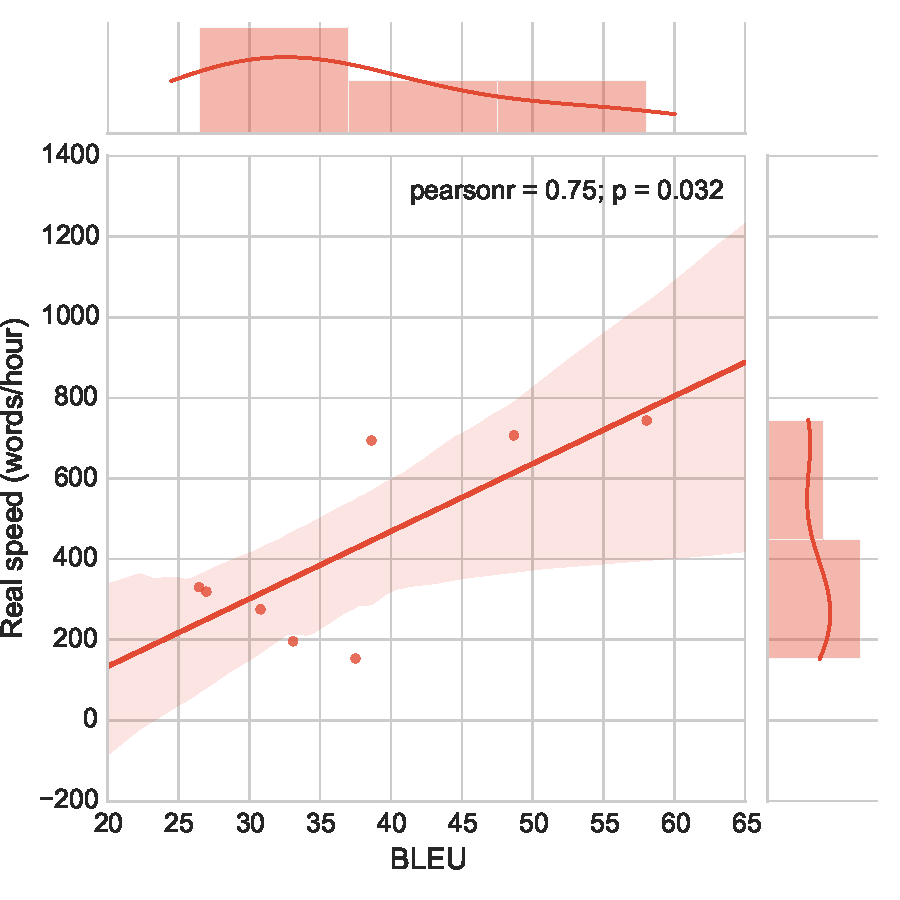
\includegraphics[width=0.45\textwidth]{img/time/time_real_bleu}}
    \subfloat[Perceived speed]{
        \label{fig:time_perceived_bleu}
    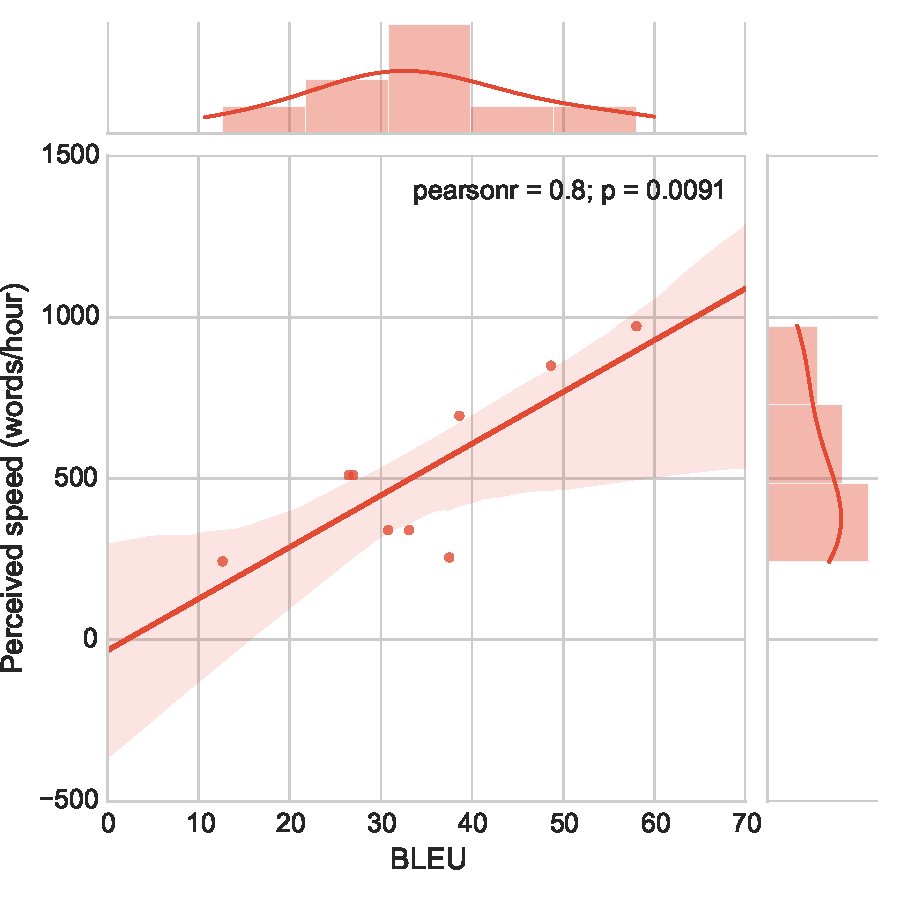
\includegraphics[width=0.45\textwidth]{img/time/time_perceived_bleu}}
    \caption{Correlation between real and perceived speed spent on post-editing and the final translation's \spacedlowsmallcaps{BLEU} score. Data from one participant was omitted from the real time as it was a clear outlier (including it, the correlation was $r = 0.39$)}
    \label{fig:time_bleu}
\end{figure}

Thus, it seems that the \ac{PE} only acheives an increase in speed when translators minimally edit the \ac{MT} suggestion. Participants were not given guidelines on how to use the \ac{MT} suggestions, so they were free to take the approach they preferred. If they feel they need to change the suggestion more, speed differences are negligible or can even result in a slow-down (\autoref{fig:time_diff_bleu}).

\begin{figure}[H]
\myfloatalign
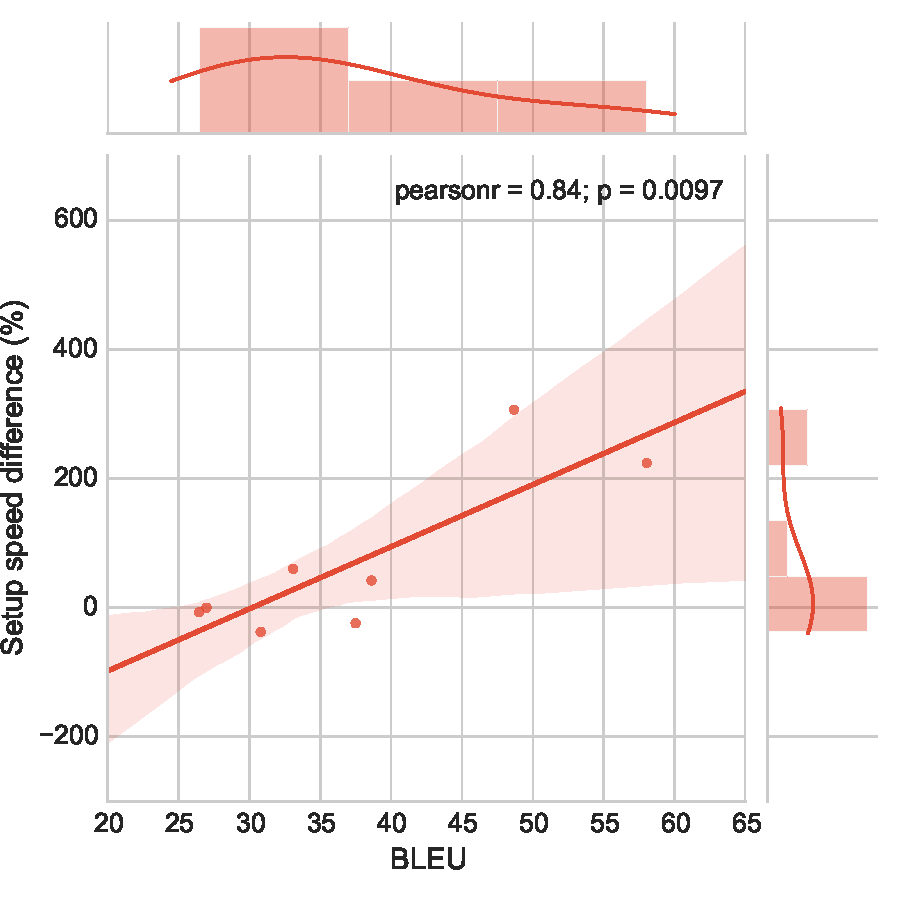
\includegraphics[width=0.5\textwidth]{img/time/time_diff_bleu}
\caption{Correlation between the \% speed difference between \scratch and \ac{PE} (positive indicates \ac{PE} was faster) and the final translation's \spacedlowsmallcaps{BLEU} scores. Data from one participant was omitted from the real speed as it was a clear outlier (including it, the correlation was $r = 0.56$)}
\label{fig:time_diff_bleu}
\end{figure}

\subsection{Perceptions of Time}

\noindent Perceived speeds have not been studied in previous literature on translation process research, thus there is no background in how to interpret them. I suggest they could also be considered a measure of effort. A tedious task raises awareness of the time being spent on it and makes people think they're spending more time on it than they actually have, while an easy and enjoyable task can seem faster. The results in this study seem to support this view. 

As can be seen in \autoref{fig:time_overall}, overall the translators thought they translated much faster than they actually did. Digging further into the data, \autoref{fig:time_real_vs_perceived} shows that participants felt that their speed between setups was roughly similar, with \ac{PE} as fastest and \style as slowest. This contrasts with the real speeds, which were roughly the same for \style and \scratch and faster for \ac{PE}.

In other words, participants were fairly accurate at predicting their time spent in \ac{PE}, but they felt \scratch and \style were faster than they actually were. This indicates that they were more aware of the time during \ac{PE}. Supposing a link between time awareness and effort, this would indicate \ac{PE} required more effort and was liked less.

\begin{figure}[h]
\myfloatalign
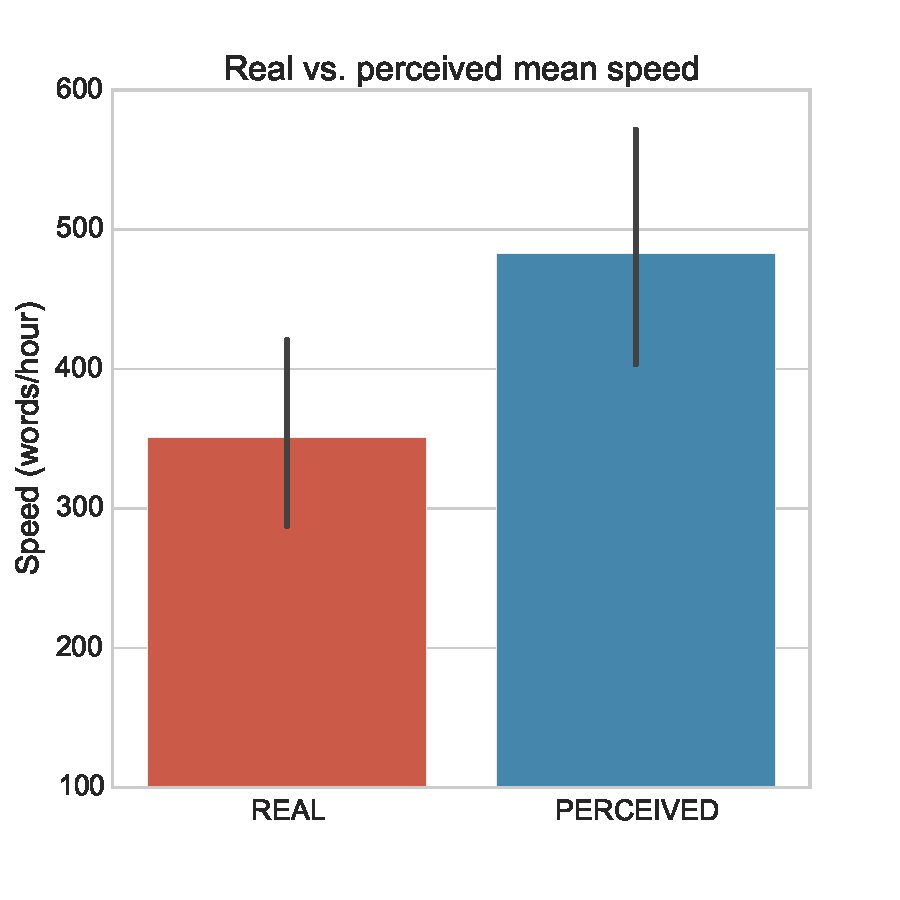
\includegraphics[width=0.5\textwidth]{img/time/time_overall}
\caption{Overall real vs. perceived mean speed. 95\,\% confidence interval calculated using bootstrap resampling.}
\label{fig:time_overall}
\end{figure}

As will be discussed in \autoref{sec:setup_prefs}, participants associated like and dislike more strongly with a particular text than with a particular setup. Looking at the speed per text in \autoref{fig:time_real_vs_perceived}, we see participants perceived \charlotte as being the slowest text to translate, which lines up with it being considered the hardest (\autoref{sub:like_dislike}). \ai was both considered the hardest (4 participants) and the second easiest (3 participants), which could explain why its average perceived speed is roughly as fast as \spacedlowsmallcaps{garfield}, which is considered the easiest translation (5 participants). 

\begin{figure}
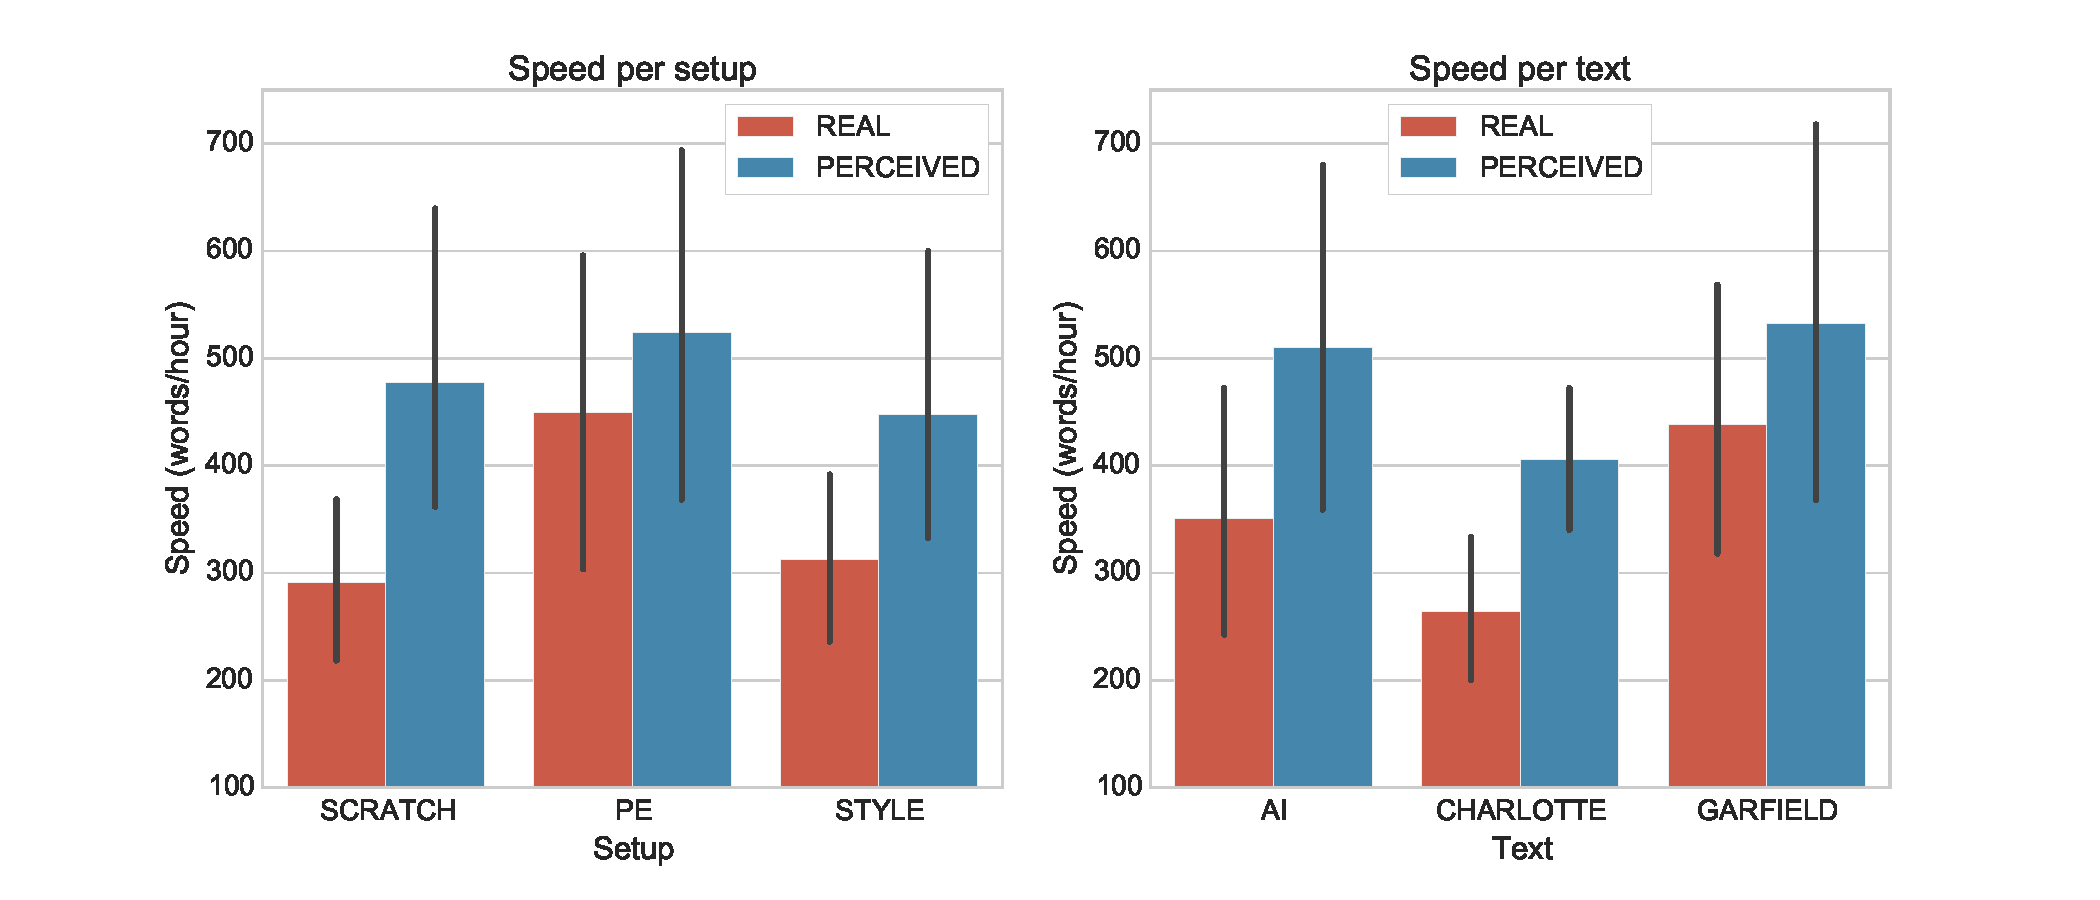
\includegraphics[width=\textwidth]{img/time/time_real_vs_perceived}
\caption{Real vs. perceived speed per setup and per text. 95\,\% confidence interval calculated using bootstrap resampling.}
\label{fig:time_real_vs_perceived}
\end{figure}

%----------------------------------------------------------------------------------------

\section{Setup Preferences}
\label{sec:setup_prefs}

\noindent In order to determine which setup the participants preferred, two key questions were asked: whether they would have preferred to translate from scratch without the \ac{MT} suggestion and without the StyleCheck hints [Questions 21 and 31]. 44\,\% said they would prefer not to have the \ac{MT} suggestions versus 33\,\% who would prefer not to have the StyleCheck suggestions. Thus, overall acceptance is higher for StyleCheck than for \ac{PE}. The acceptability rate for \ac{PE} was higher among this study's participants than in other studies such as in \textcite{carl2015post}, where 83\,\% of participants responded preferring translating from scratch. \textcite{carl2015post} does report a higher satisfaction rate for the \ac{PE} task among students versus professionals. Since this study's participants had limited experience as translators ($<2$ years), they could be considered closer to the student category than the professional category. This could explain the higher acceptability rate.

\subsection{Satisfaction}

\noindent Participants were asked to rate their satisfaction both for the task and the quality of their final translation for each setup [Questions F.14-15, F.22-23, F.32-33]. Task satisfaction results in \autoref{tab:satisfaction} indicate that \ac{PE} was the most satisfactory setup, followed by \scratch and \style in final place. Quality satisfaction results (\autoref{tab:satisfaction}) indicate a similar trend, with \ac{PE} providing the highest quality satisfaction, followed by \style and then \spacedlowsmallcaps{scratch}. These results seem to be in direct opposition to those discussed in the previous paragraph, where the majority of participants preferred the \scratch setup, followed by \style and \ac{PE}. It should be noted, however, that the means are always between 1 and 3, indicating participants were not dissatisfied with any of the setups or resulting quality.

\begin{table}[h]
    \subfloat[Task satisfaction]{
        \label{tab:sat_task}
        \begin{tabularx}{0.45\textwidth}{Xcc}
            \toprule
            \tableheadline{Setup} & \tableheadline{Mean rating} & \tableheadline{\sigma} \\
            \midrule
            \scratch &  $2.2$ & $0.4$\\
            \ac{PE} &  $1.9$ & $0.6$ \\
            \style &  $2.4$ & $0.9$ \\
            \bottomrule
    \end{tabularx}}
    \quad
    \subfloat[Quality satisfaction]{
        \label{tab:sat_quality}
        \begin{tabularx}{0.45\textwidth}{Xcc}
            \toprule
            \tableheadline{Setup} & \tableheadline{Mean rating} & \tableheadline{\sigma} \\
            \midrule
            \scratch &  $2.7$ & $0.9$\\
            \ac{PE} &  $1.9$ & $0.8$ \\
            \style &  $2.4$ & $1.2$ \\
            \bottomrule
    \end{tabularx}}
    \caption{Mean ratings and standard satisfaction ratings with the task and the final translation quality broken down by setup. Ratings range from 1 (Very satisfied) to 5 (Very dissatisfied).}  
    \label{tab:satisfaction}
\end{table}

\begin{table}[h]
    \subfloat[Task satisfaction]{
        \label{tab:sat_task_text}
        \begin{tabularx}{0.45\textwidth}{Xcc}
            \toprule
            \tableheadline{Text} & \tableheadline{Mean rating} & \tableheadline{\sigma} \\
            \midrule
            \ai &  $2.4$ & $0.7$\\
            \charlotte &  $2.4$ & $0.7$ \\
            \garfield &  $1.9$ & $0.6$ \\
            \bottomrule
    \end{tabularx}}
    \quad
    \subfloat[Quality satisfaction]{
        \label{tab:sat_quality_text}
        \begin{tabularx}{0.45\textwidth}{Xcc}
            \toprule
            \tableheadline{Text} & \tableheadline{Mean rating} & \tableheadline{\sigma} \\
            \midrule
            \ai &  $2.7$ & $0.9$\\
            \charlotte &  $2.4$ & $1.0$ \\
            \garfield &  $1.9$ & $1.1$ \\
            \bottomrule
    \end{tabularx}}
    \caption{Mean ratings and standard deviation for satisfaction ratings with the task and the final translation quality broken down by text. Ratings range from 1 (Very satisfied) to 5 (Very dissatisfied).}  
    \label{tab:satisfaction_text}
\end{table}

We hypothesise that the result disparity just described is due to participants linking satisfaction more strongly to the texts that were translated rather than the setups they were translated in. \autoref{tab:satisfaction_text} shows the results of braking the satisfaction down by text. \garfield always comes out top, which is in line with it being the most liked text (\autoref{sub:like_dislike}). A larger participant pool would be required to obstain more conclusive results.

\subsection{Like/Dislike, Easy/Difficult and Control}
\label{sub:like_dislike}

\noindent To provide more context to the satisfaction ratings, participants were asked what they liked or disliked about the setups [Questions F.12-13, F.18-19, F.26-27]. They were also asked what translations where the hardest and the easiest [Questions F.3-6] and during which setups they felt they had the most and least control [Questions F.7-10]. We discuss each of these separately.

The majority of participants mentioned textual considerations as a factor in deciding whether a text was easy or hard [Questions F.3-6]. These included text structure, topic, terminology, etc. When asked why a text/setup was hard, one participant complained that editing the \ac{MT} suggestion doubled the amount of work compared to translating from scratch. When asked why they had chosen a text/setup as the easiest, two participants mentioned that post-editing an \ac{MT} suggestion was faster and easier. When braking down the results by text, \garfield is mentioned as the easiest (56\,\% of participants) and is the chosen the least times as the most difficult (only one participant). \charlotte turns out to be the most difficult if we combine that it's in joint first place for the most difficult (\ai and \charlotte have 4 counts each) and it receives just a single count as the easiest.

The case of the AI is interesting. Considered both the hardest (4 participants) and the second easiest (3 participants) to translate, the data shows no correlation between its hard/easy consideration and having translated it in a particular setup. This further strengthens the view that difficulty is linked to a certain text rather than a certain setup, although as previously mentioned setups can play a part in this.

As for what was liked or disliked, participants mentioned more frequently in their open answers aspects relating to the text topic or specific textual elements. Specifically, \garfield seems to have been the text most liked by participants. The quality and usefulness of the \ac{MT} suggestions also appear fairly frequently. Once again, it seems that the texts have more of an influence on what participants liked or disliked than specific. 

Finally, the data on control or lack of it paints a similar picture. When asked where they felt they had the most control [Question F.7-8], responses were spread equally among setups but showed great variation in texts: \garfield made them feel most in control, followed by \ai and \charlotte. Open answers present as reasons a mix of textual considerations (participants knew a lot about Garfield, there were no tricky terms) and setup considerations (some disliked have suggestions or hints of any kind). As for where they had least control [Questions F.9-10], results again show a flat variation among setups but differences in texts: \ai made them feel the least in control, followed by \charlotte and \garfield. Here, the open answers overwhelmingly mention textual considerations such as the topic and terminology.

\subsection{Causes}

\noindent To throw further light onto the high acceptance of the \ac{PE} setup, we can look at the quality ratings for the \ac{MT} suggestions. Following \textcite{carl2015post} and what is commonplace in \ac{MT} evaluation, participants were asked to rate the \ac{MT} quality on three criteria: grammaticality, style and accuracy [Question F.20]. Results (\autoref{tab:mt_eval}) show all three criteria were considered average, edging towards above average. There were even some counts of well above average grammaticality (1 count) and style (1 count). This in contrast to participants in \textcite{carl2015post}, who rated all criteria closer to below or well below average. A perceived higher quality of the \ac{MT} suggestions explain the higher acceptance of \ac{PE} in this study. As for the \style setup, further discussion is provided in \autoref{sec:sc_effectiveness}.

\begin{table}[h]
\myfloatalign
\begin{tabularx}{0.5\textwidth}{Xcc}
\toprule
\tableheadline{Criteria} & \tableheadline{Mean rating} & \tableheadline{\sigma} \\
\midrule
Grammaticality &  $2.7$ & $1.0$\\
Style &  $2.6$ & $0.7$ \\
Accuracy &  $3.0$ & $1.0$ \\
\bottomrule
\end{tabularx}
\caption{Mean ratings and standard deviation for \ac{MT} quality evalutaions. Ratings ranged from 1 (Well above average) to 5 (Well below average), with 3 being Average.}
\label{tab:mt_eval}
\end{table}

\subsection{Summary of Preferred Setups}

\noindent Thus, after the previous considerations, the data indicated that participants' preferred setup was \spacedlowsmallcaps{scratch}, followed by \style and \ac{PE}. This is essentially based on Questions F.21 and F.31.

The previous findings also make it is reasonable to suppose that participants perceive the specific text (topic and textual considerations) as having the most influence in their preferences and enjoyment of a translation (degree of easiness, like/dislike, and task and quality satisfaction). This is useful insight for designing questionnaires whose aim is to evaluate a tool. Although the free form answers do provide some insight into the tool, it is best evaluated with a direct question of the kind ```Whould you have preferred to translate without $X$?''.

%----------------------------------------------------------------------------------------

\section{StyleCheck Effectiveness}
\label{sec:sc_effectiveness}

\noindent This section evaluates the efectiveness of StyleCheck by analysing the actual translations produced by the participants. Before delving into the details, it is important to determine whether participants considered that sticking to the Wikipedia \ac{SG} rules was important (just as the translation brief stated it was).

\subsection{Style Guide Importance}

\noindent Participants were asked if they had established any priorities and restrictions after reading the brief and, if yes, which ones [Questions F.1 and F.2]. The notion of priorities and restrictions is taken from \textcite{zabalbeascoa1999priorities}, and describes the hierarchical list of aims and goals that translators establish for a translation after taking all factors into account (\ac{ST}, target culture, client requirements, deadline and even pay). 67\,\% reported having established priorities and restrictions. Out of these, half explicitly mentioned following the Wikipedia Style Guide as their top prority. One participant mentioned specific aspects of the writing style used in Wikipedia, and the rest mentioned general strategies of translation. Thus, the translation brief succeeded in making most participants prioritise style guide application. The others may have not prioritised it considering that the translations were short and they were not receiving compensation for the experiment, making it not worth the time and effort to read the whole style guide and follow it. This would also fit in with the model of priorities and restrictions, which as mentioned before allows for time and payment considerations to come into play.

Participants were asked if they had consulted the Wikipedia style guide linked in the brief [Question F.28]: 67\,\% said they had. Logging carried out on the server indicates the link to the Wikipedia Style Guide was only clicked by a third of the participants, one of which answered that they hadn't consulted the style guide. This could be due to participants opening up a new tab and searching for the style guide themselves, but given that the link was provided on all translation pages, this seems unlikely. It seems participants felt they should have consulted it, but preferred to say they had when they actually had not. This is a strong indicator of the usefulness of a digitally applied style guide: participants felt compelled to apply it, but did not. As stated before, this was probably due to the lack of time and short texts which did not make up for the investment in time required to read and apply the style guide.

When asked why [Question F.29], those who hadn't consulted the guide said they were not used to using style guides or that they had previously translated Wikipedia articles and were familiar with it. Those who had, either stated the general importance of using a style guide when one is provided by a client or mentioned specific elements they looked up (use of italics, parenthesis, how to handle names of works of art, etc.).

\subsection{Style Guide Application}

\noindent To evaluate how well StyleCheck worked, we first look at the objective data of whether a particular rule was applied or not in each translation. \autoref{fig:rules_1a} presents how many times the rules identified in the texts were applied or not. The \spacedlowsmallcaps{mixed} category refers to elements that appear more than once in a single text and present inconsistencies: some instances follow the associated style rule, others don't. The \spacedlowsmallcaps{avoided} category refers to instances where the text was changed, resulting in the rule issue being avoided. As can be seen, the \style setup leads to a notably higher amount of rules applied than the other setups. This is further confirmed in \autoref{fig:rules_1b}, which shows the data only for rules that were implemented in StyleCheck.

\begin{figure}[h]
\subfloat[Total rules]
{\label{fig:rules_1a}
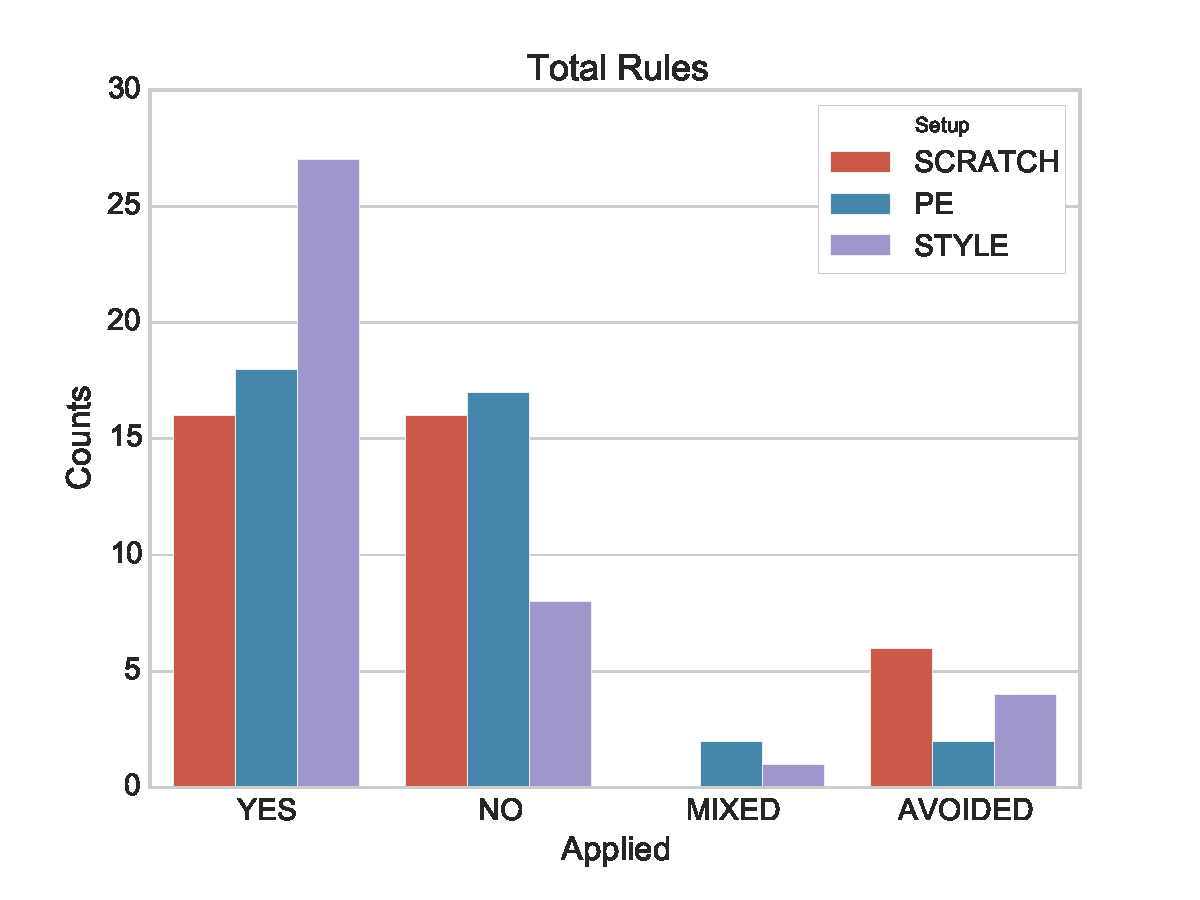
\includegraphics[width=0.5\textwidth]{img/rules/rules_1a}}
\subfloat[Rules implemented in StyleCheck]
{\label{fig:rules_1b}
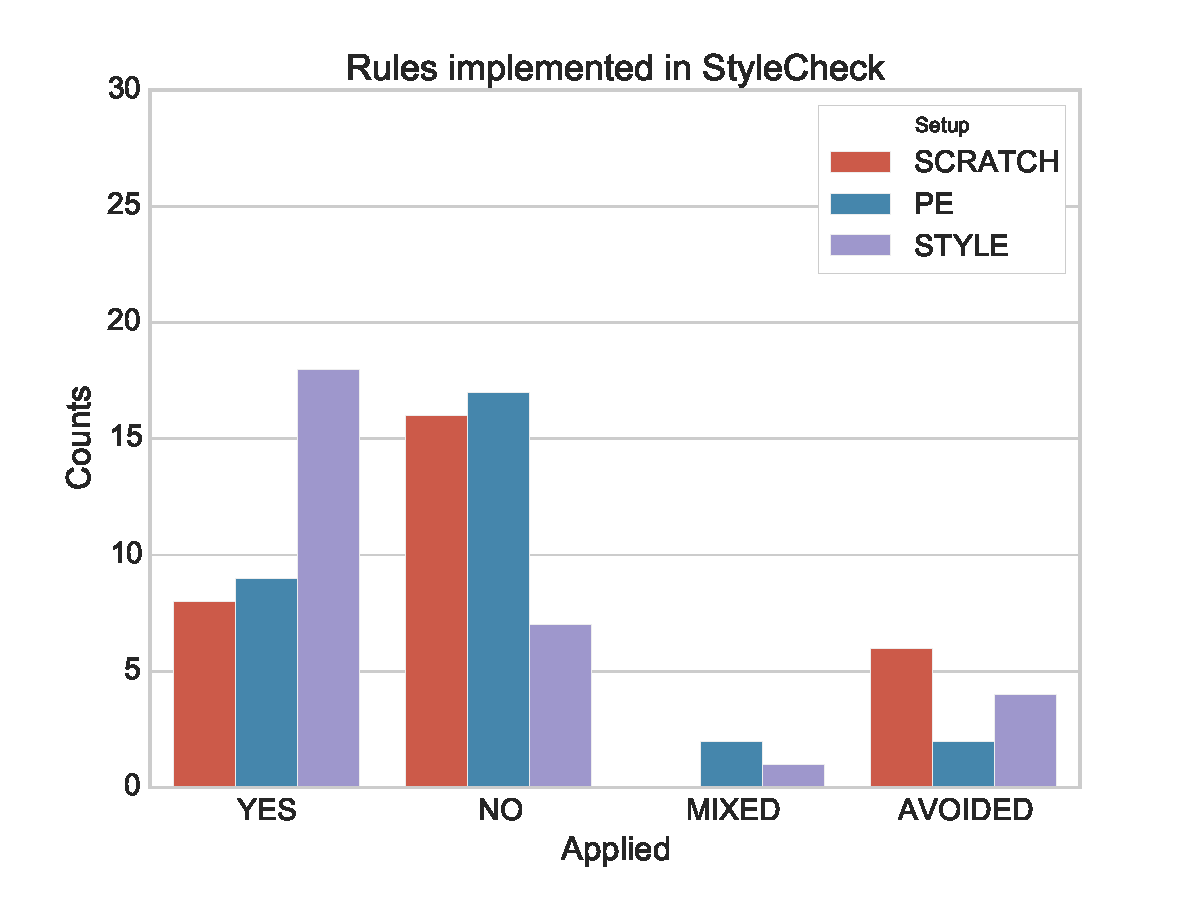
\includegraphics[width=0.5\textwidth]{img/rules/rules_1b}}
\caption{Number of rules that were applied in the final translations. Both the total number of rules detected in the texts and the subset of rules implemented in StyleCheck are presented.}
\label{fig:rules_1}
\end{figure}

Rule application varied a lot depending on the particular rule, as can be seen in \autoref{fig:rules_2}. Some rules, such as \spacedlowsmallcaps{3b} and \spacedlowsmallcaps{3c} were always applied. They were related to aspects (number formatting) that translators usually know are contained in style guides and may have previous experience in how to handle. Others, such as \spacedlowsmallcaps{2a} and \spacedlowsmallcaps{2b} were generally not applied. These were related to aspects very specific to the Wikipedia style guide (chronologiclly ordering lists and avoiding time expressions that refer to the moment of enunciation).

\begin{figure}[H]
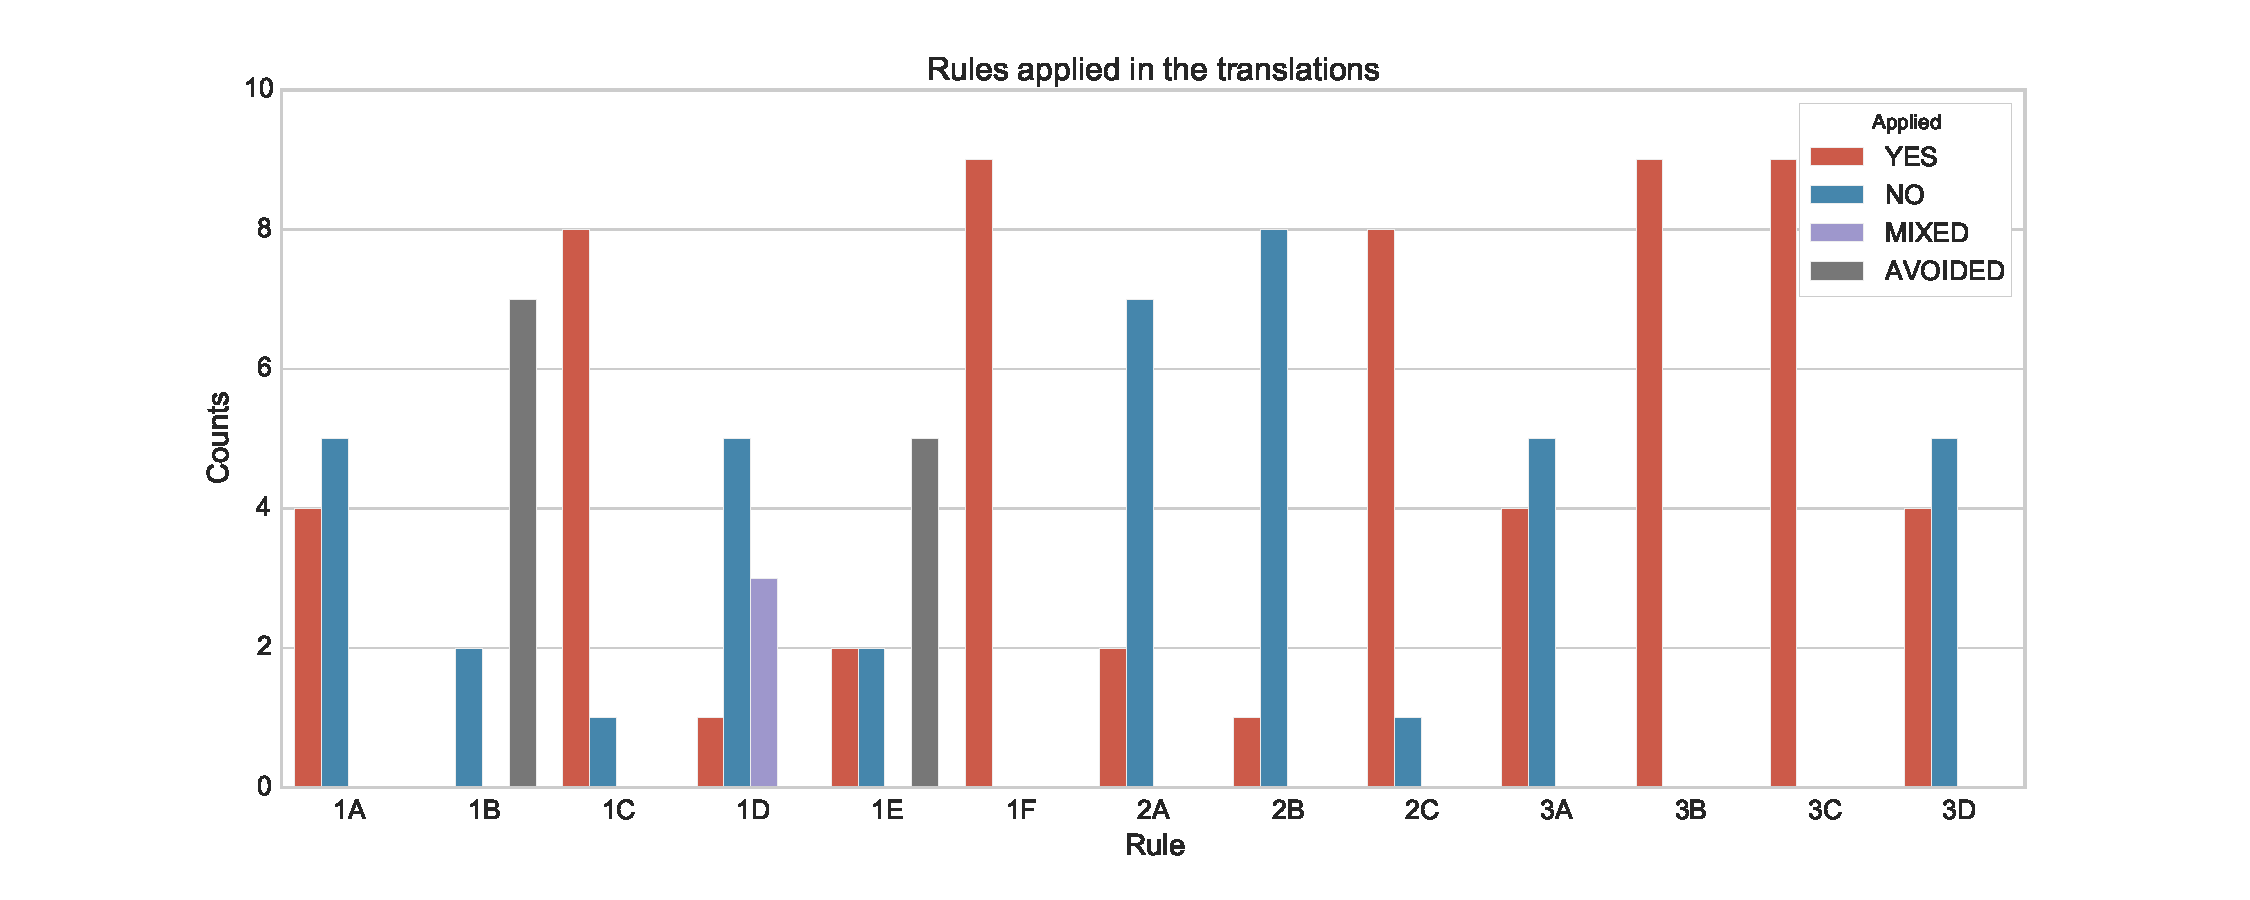
\includegraphics[width=\textwidth]{img/rules/rules_2}
\caption{Number of rules applied in the final translations for all setups. Counts are broken down by rule.}
\label{fig:rules_2}
\end{figure}

\subsection{StyleCheck vs. \ac{PE}}

\noindent We now turn to a comparison of the \style and \ac{PE} setups. Starting off with \ac{PE}, we find that participants tended to closely follow what the \ac{MT} suggestion presented. \autoref{fig:rules_3a} shows that all instances of rules that were applied in the \ac{MT} suggestion were also applied in the final translation. \autoref{fig:rules_3b} shows similar results: 67\,\% of rules not applied in the suggestion were not applied in the final translation. Only 25\,\% of them were corrected so that they were correctly applied. The mixed instances in the \ac{MT} suggestion provide further evidence: two out of the three instances were also carried on to the final translation. With a simple revision of the final translation, participants should have noticed the inconsistencies and homogenised them.

\begin{figure}[H]
\myfloatalign
\subfloat[Rules applied in \ac{MT}]
{\label{fig:rules_3a}
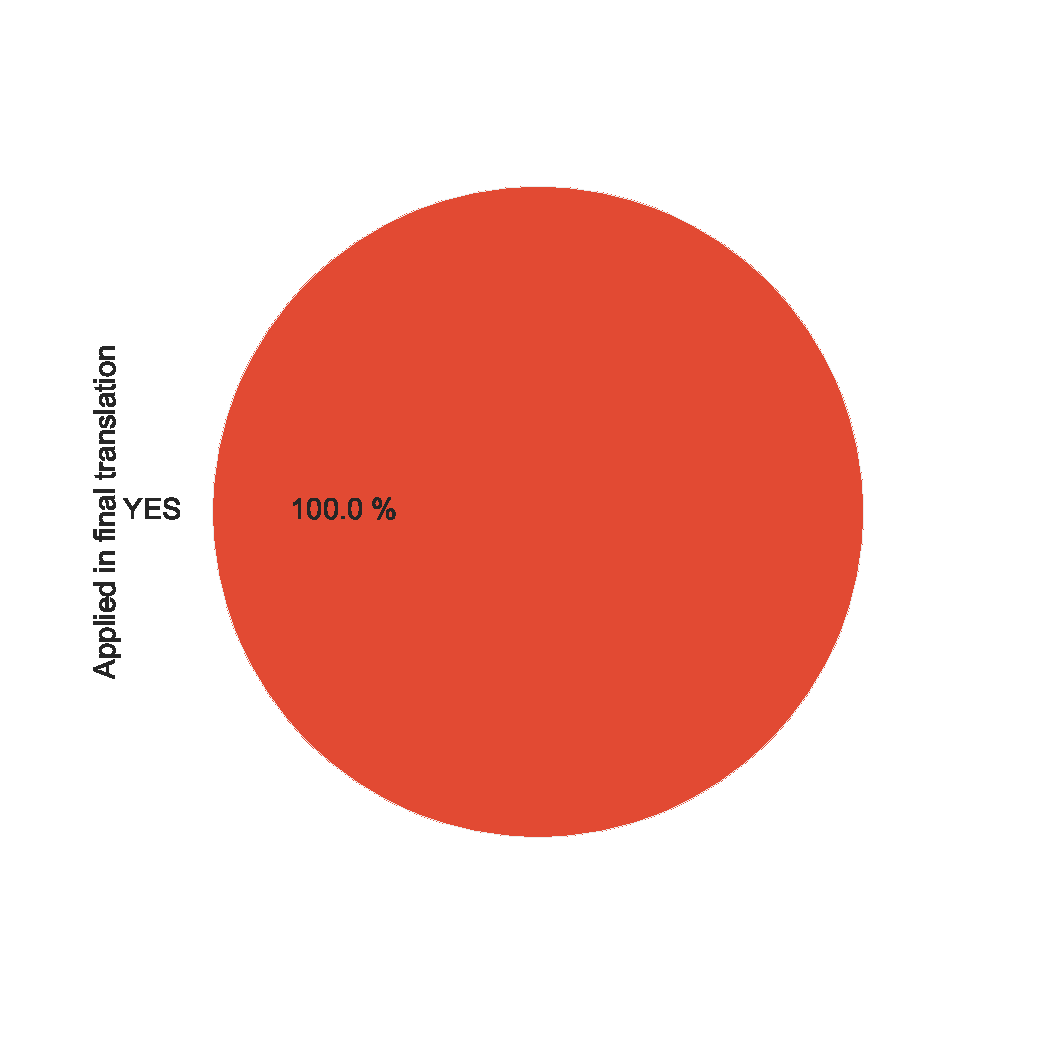
\includegraphics[width=.45\linewidth]{img/rules/rules_3a}}
\subfloat[Rules not applied in \ac{MT}]
{\label{fig:rules_3b}
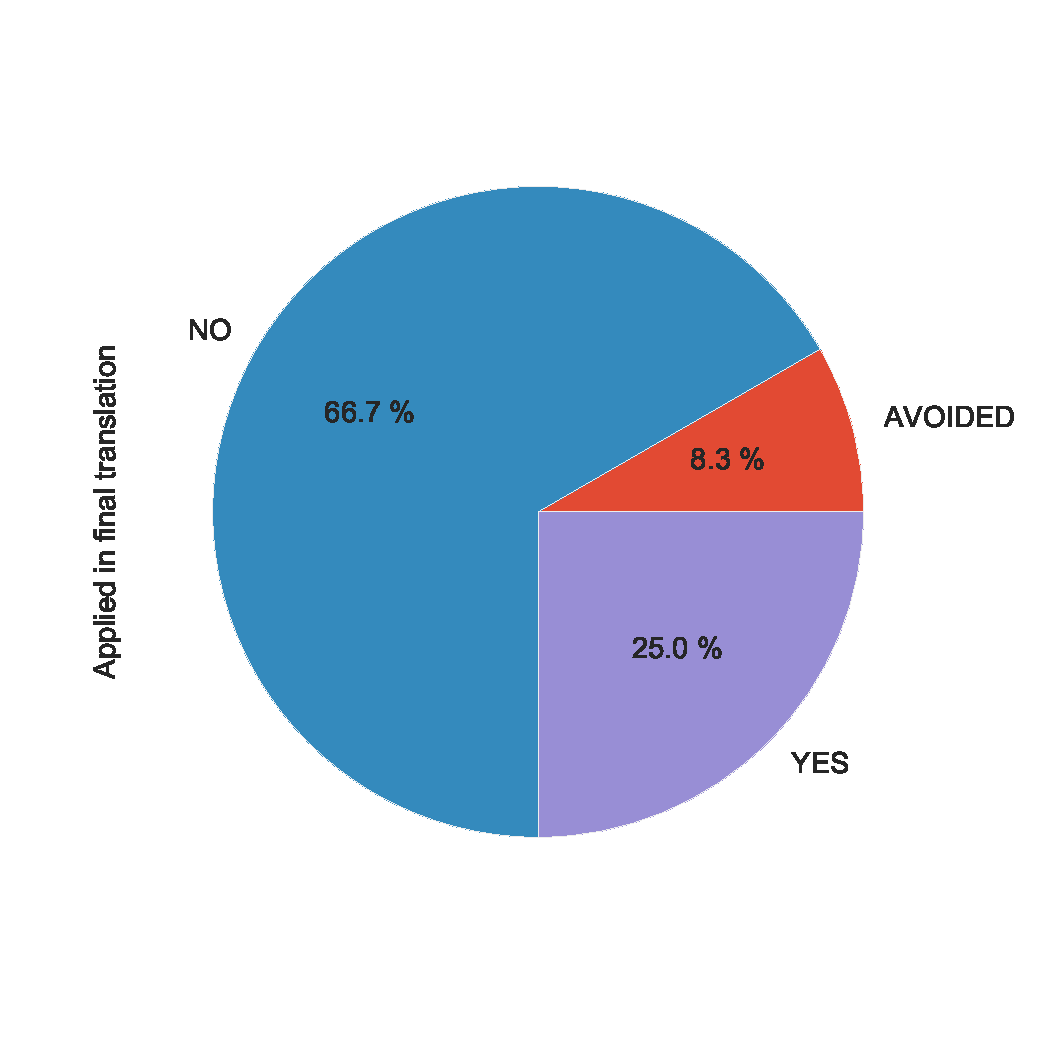
\includegraphics[width=0.45\linewidth]{img/rules/rules_3b}}
\caption{Percentage of rules applied or not in the final translation for the \ac{PE} setup depending on whether the\ac{MT} suggestion had applied them or not.}
\label{fig:rules_3}
\end{figure}

Delving further in the data, we find that StyleCheck was effective in getting participants to follow the suggestions. When presented with a suggestion (indicating the participant had written a sentence that did not follow a specific rule), 71\,\% of the time participants corrected their translations so that they followed the suggestion. 

To find out why in 29\,\% of the cases the suggestions weren't followed, we can check two sources of data, objective and subjective. Objective data indicates that out of the five cases where the suggestion wasn't followed, in two cases the relevant suggestion was shown in third position below two other suggestions. It is possible that depending on the screen resolution and browser window configuration the suggestion appeared outside of the screen and was not seen or ignored. The fact that some suggestions were long could have also contributed to this. A further two cases presented the suggestion in first position, indicating the participant ignored the suggestion or chose not to follow it. 

Subjective data was collected through the final questionnaire [Question F.30] and is presented in \autoref{tab:sc_eval}. Participants rated their agreement with various satements from 1 to 5. Participants generally agreed that the style hints were helpful, and agreed that the information they contained was right. Results show participants generally thought the style hints were easy to understand, but tended to agree that they were too long. This would suggest the hints could be improved by rewriting them into a tenser alert style, rather than copy the original style guide description. Regarding the user interface, participants on average remained rather neutral on whether there were too many hints and whether the boxes were distracting. However, both considerations included one instance of a participant strongly agreeing.


\begin{table}[h]
\myfloatalign
\begin{tabularx}{\textwidth}{Xcc} \toprule
\tableheadline{Consideration} & \tableheadline{Mean agreement} & \tableheadline{\sigma} \\
\midrule
The style hints were helpful & $2.3$ &  $1.0$ \\
There were too many style hints & $2.8$ & $1.1$ \\
The style hints were easy to understand & $1.6$ & $0.7$ \\
The style hints were too long & $2.1$ & $1.1$ \\
The boxes where the style hints were shown were distracting & $2.6$ & $1.1$ \\
The style hints contained wrong information & $3.7$ & $1.0$ \\
\bottomrule
\end{tabularx}
\caption{Mean agreements and standard deviations for whether participants agree or not with various statements related to the StyleCheck suggestions. Ratings range from 1 (Strongly Agree) to 5 (Strongly Disagree).}  
\label{tab:sc_eval}
\end{table}



%----------------------------------------------------------------------------------------

\section{Future Work}


\subsection{Two Types of PE}

\noindent The data revealed that \ac{PE} seems to only improve translation speed when little editing is done, what has been called light \ac{PE}. Full \ac{PE}, on the other hand, doesn't necessarily amount to a large speed improvement and forces a workflow on translators that some dislike in comparison to translating from scratch. Thus, I would classify light \ac{PE} under human-assisted \ac{MT}, where the main structure and choices in the translation are selected by the system. Full \ac{PE} would fall into the \ac{CAT} category, but more research is required into this variant to see if the slow-downs and small speed improvements also appear in larger studies. If they do, it could question the usefulness of \ac{PE} for full-quality translation.

\subsection{TPR Methodology}

\noindent Within the space of verbal report data, there is a need for standardised set of questions to make comparisons across studies possible. The \spacedlowsmallcaps{CRITT TPR-DB} \parencite{carl2012critt} database already does this for data such as keylogging, time, eye-tracking and other measurements, but verbal-report data in the form of questionnaires, for example, is completely left out. As this thesis has shown, this information is key in providing context to the data collected from logging and tracking of all kinds. Future studies should work in the direction of trying to use similar questions and analysing the data in a similar fashion.

\subsection{StyleCheck: Improvements}

\noindent The questionnaires brought up a few issues with the suggestion interface StyleCheck uses. Notably, it would be better for the text to be shorter and more to the point. Future versions of StyleCheck should rewrite the raw text included in a style guide to better adapt to the needs of a quick suggestion, which could include a link to the full description if needed. Another area of improvement is with regards to the always-on suggestions. Some participants stated they would prefer to completely dismiss a suggestion or all of them, so this functionality should be included. Optionality of StyleCheck itself is also important given that a number of participants stated they would have preferred to translate without them. 


\subsection{StyleCheck: MT Evaluation Metric and Beyond}

\noindent The \ac{GF}-based approach to implementing style guides can be useful for other tasks. The most interesting and useful is as a metric for \ac{MT} evaluation. StyleCheck can be turned into a metric which operates in a similar fashion to unit testing in the software development world.

Style guides, as part of a translation brief, encode requirements and expectations the translation has to fulfill. These requirements are embodied in isolated \ac{GF} functions that can be individually checked to see whether a rule was applied or not. \ac{GF} is flexible enough to allow many different kinds of rules to be created and check whether many linguistic aspects appear in a text or not. An \ac{MT} metric can be built upon this basis, checking each translation for all the aspects relevant to a particular client, domain, text type, etc. Thus, the notion of ``quality'' becomes flexible and adaptable according to translator, client and situational needs, more in-line with the skopos paradigm in translation theory.

This metric would have numerous advantages. It would allow to see what specific aspects a translation failed in. Through attaching a weight to each aspect, a hierarchy can be established to prioritise particular aspects over others, in a similar way to the model of priorities and restrictions \parencite{zabalbeascoa1999priorities}. Once the metric is defined, it can be used to rank candidates output by a decoder in an \ac{SMT} system or translation options from multiple systems, as well as being used in \ac{SMT} tuning.

Lastly, StyleCheck can also be used for automatic post-editing of certain aspects that don't require translator intervention, as explained in \autoref{ch:stylecheck}.
 % Chapter 10
\chapter{Conclusion}

\label{ch:conclusion}

\noindent This thesis has presented a unified methodology for developing and evaluating \ac{CAT} tools. The methodology has then been used to develop StyleCheck, a tool that helps translators by giving them hints about style guide rules that should be applied while they are translating.

%----------------------------------------------------------------------------------------

\section{StyleCheck}

\noindent Results show StyleCheck acheived its main goal: leading to a higher rate of rule application. Using it lead to more style rules being applied when compared with translation from scratch and post-editing.

StyleCheck does not seem to burden the translation process. Translators prefer it to post-editing. Speed is comparable to from-scratch translation, but the \spacedlowsmallcaps{UI} needs some work. Although not considered distracting nor intrusive, the interaction can be improved upon, especially with regards to adapting and rewriting the style guide rules to make them terser.

Despite the advantages, developing the rules themselves requires a lot of manual work. Inventoring all the options that a rule should match can be tricky, and some instances can fall through the net. 

%----------------------------------------------------------------------------------------

\section{Methodology}

\noindent The \ac{CAT} tool development methodology described in this thesis proved its worth. A simple survey among translators came up with plenty of suggestions for \ac{CAT} tool improvements, as did a quick read through translation theory.

Methods developed in \ac{TPR}, when used in combination (triangulation), managed to generate a wealth of data into many aspects of a tool: how translators use it, how it affects the way they translate and the impact on the final translation. This was possible even considering the only the most basic \ac{TPR} methods were used; more advanced methods such as eyetracking and keylogging should further improve understanding of how a tool is used.

As for specific findings related to evaluation, it has been shown that in questionnaires it is best to avoid questions related to ease/difficulty or like/dislike, as the text itself can weigh more heavily than the setup used. It is thus recommended to use questions that directly ask if translators would prefer to translate without a certain tool.

Continuing on the topic of evaluation, time as a metric should be used with care. Other studies that claim speed improvements in some setups or using certain tools fail to consider translation as a whole and ignore time-consuming tasks. Data presented in this thesis showed that post-editing speed increases only apply to the light variant with minimal changes. Full post-editing, where it is used as a \ac{CAT} tool, doesn't show large speed-ups and can even slow down some translators.

Prototyping as used in this thesis to develop StyleCheck is shown to be very useful as a feedback loop. A relatively modest investment in time and effort to build a prototype still manages to generate sufficient data about how the full tool will perform. Prototyping also allowed for problems with the tool (such as the hints being too long and always-on) to surface at an early stage so they can be quickly fixed.

All in all, work carried out in this thesis provides solid ground for the \ac{CAT} tool development methodology to be adopted and used in future research.
 % Chapter 11

\cleardoublepage % Empty page before the start of the next part

%----------------------------------------------------------------------------------------
%	THESIS CONTENT - APPENDICES
%----------------------------------------------------------------------------------------

\appendix

\part{Appendix} % New part of the thesis for the appendix

% Appendix C

\chapter{Experiment Walkthrough}
\label{an:walkthrough}

%----------------------------------------------------------------------------------------

\noindent The following are screenshots of each page of the experiment website. First, participants were greeted and given an overview of the experiment procedure (\autoref{fig:web_main}). Next, participants were asked to complete the initial questionnaire (\autoref{fig:web_initial}). After submitting it, they were presented with the translation brief for the three translation tasks on a page on its own (\autoref{fig:web_brief}). The aim was for participants to read it and pay attention to it before starting the translations. Participants were told that the brief would be available on the following pages should they need to read it again.

\begin{figure}[h]
\myfloatalign
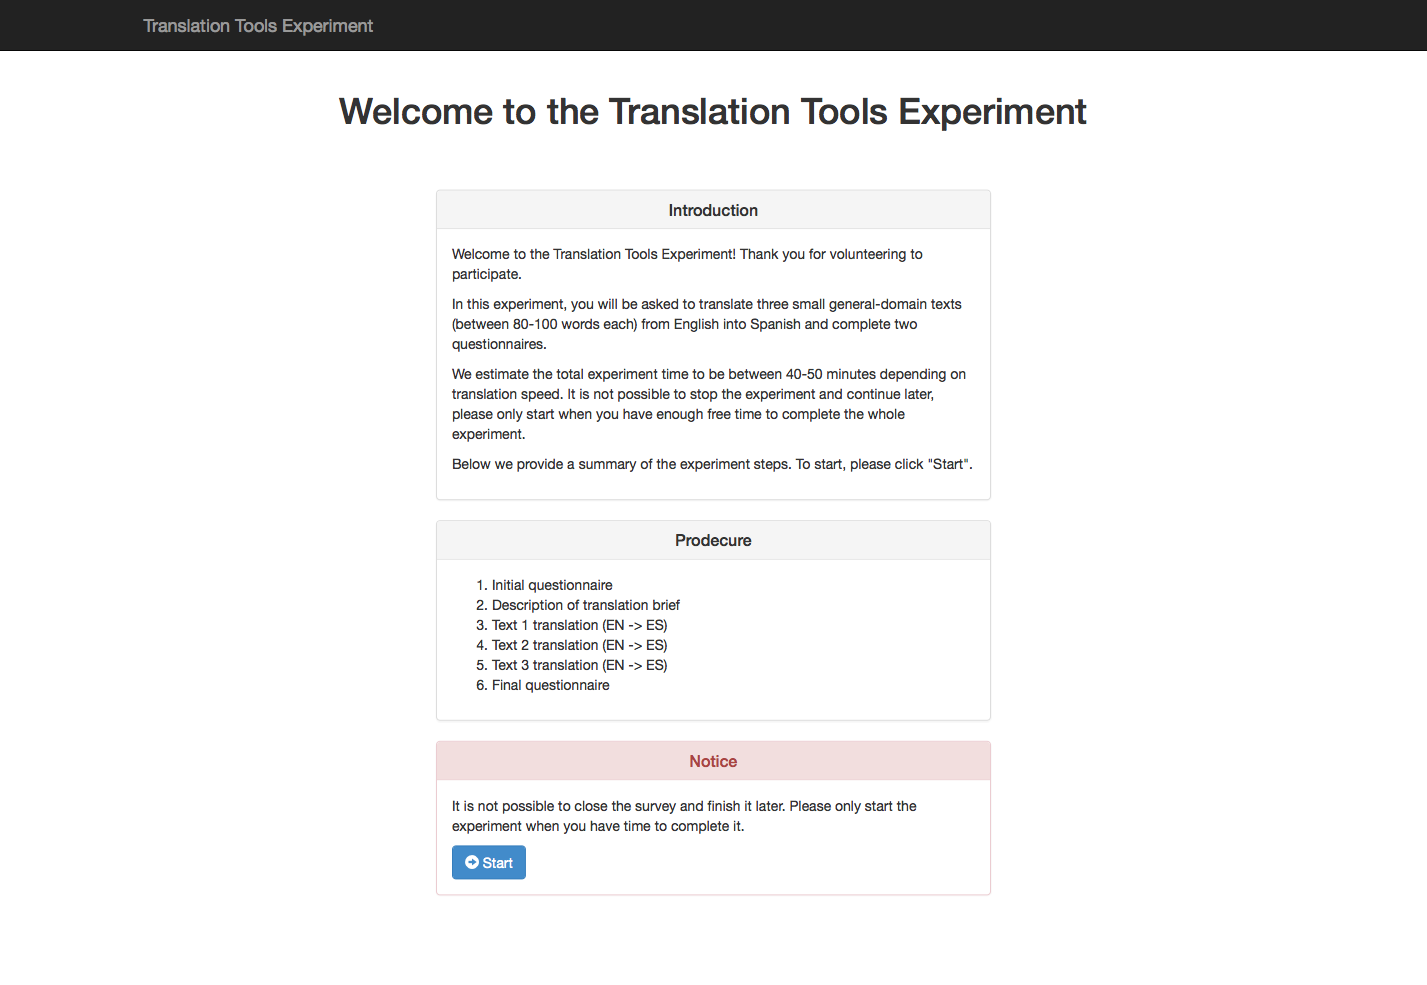
\includegraphics[width=\textwidth]{img/web/web_1.png}
\caption{Website (Page 1). Main page with a general overview of the experiment.}
\label{fig:web_main}
\end{figure}

\begin{figure}[h]
\myfloatalign
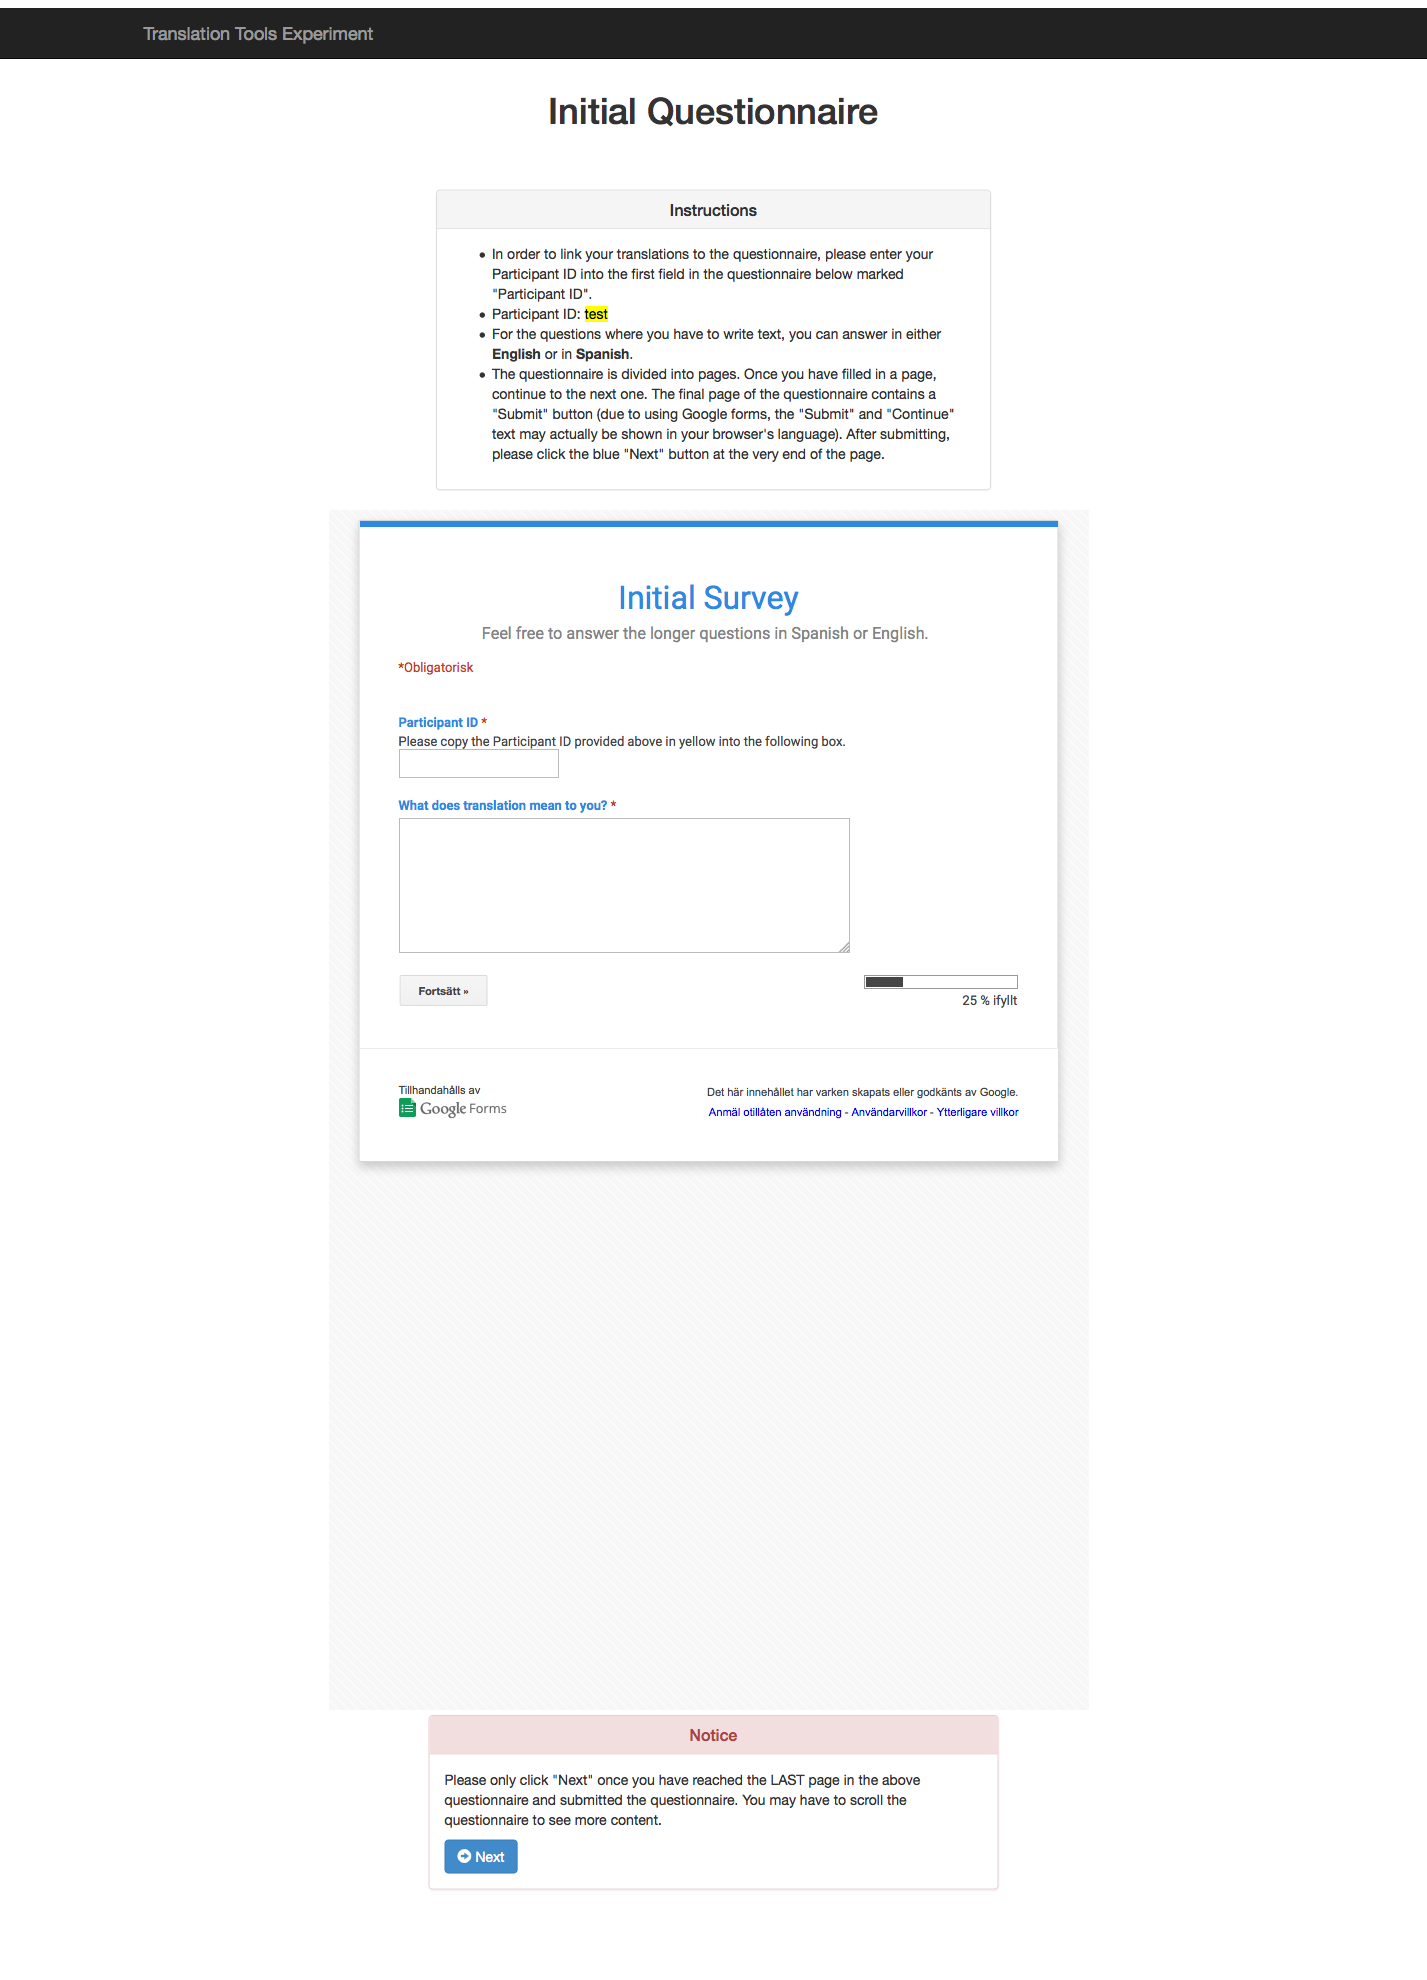
\includegraphics[width=\textwidth]{img/web/web_2.png}
\caption{Website (Page 2). Participants answer the initial questionnaire.}
\label{fig:web_initial}
\end{figure}

\begin{figure}[h]
\myfloatalign
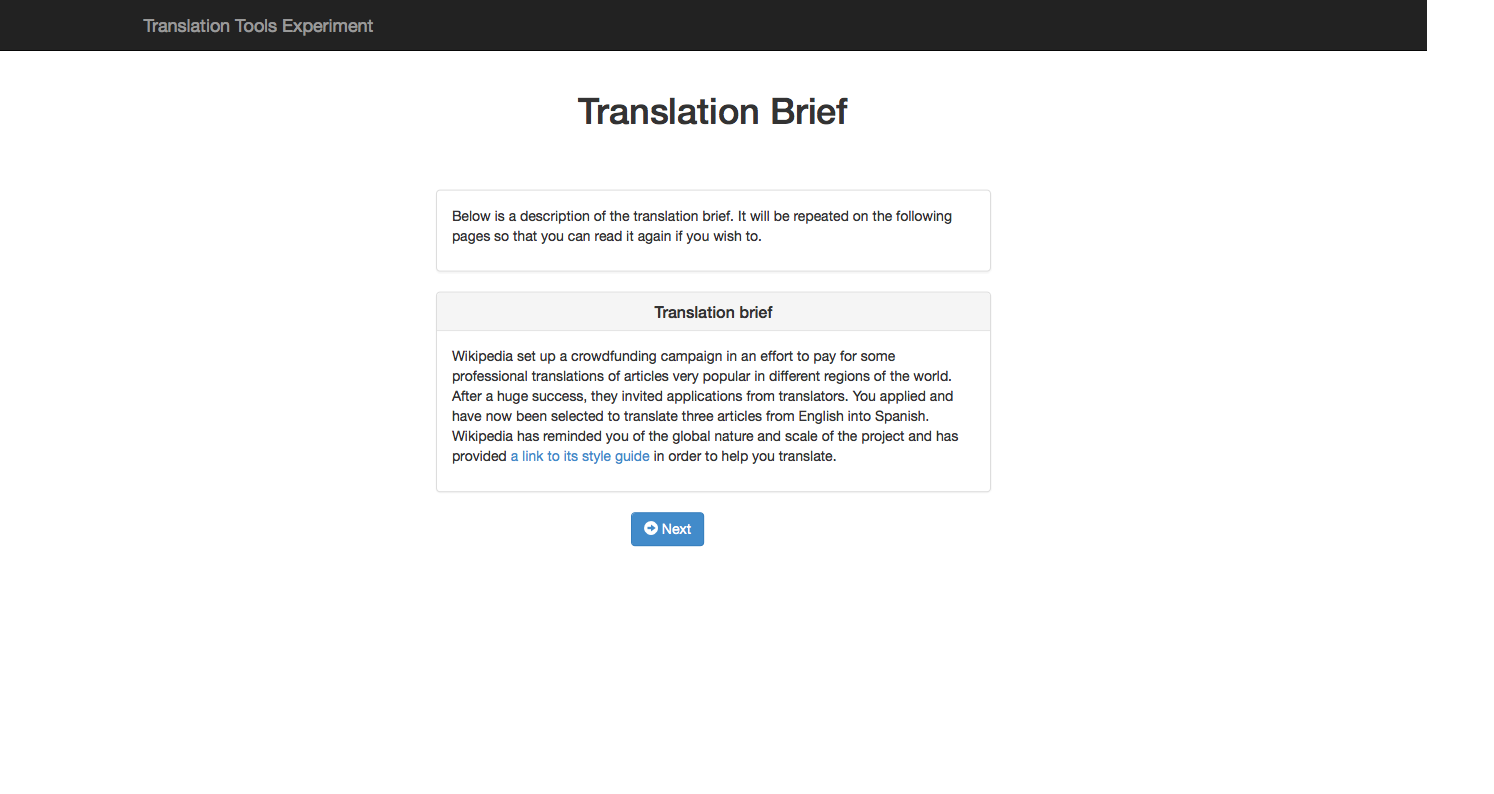
\includegraphics[width=\textwidth]{img/web/web_3.png}
\caption{Website (Page 3). Translation brief description.}
\label{fig:web_brief}
\end{figure}

Then, participants had to carry out the three translations. At the top of each page, instructions were provided for each setup and the translation brief was included. First, the \scratch setup (\autoref{fig:web_scratch}). Second, the \ac{PE} setup (\autoref{fig:web_pe}). Third, the \style setup (\autoref{fig:web_style}). The texts were presented according to the order participants had been provided in the initial link.

\begin{figure}[h]
\myfloatalign
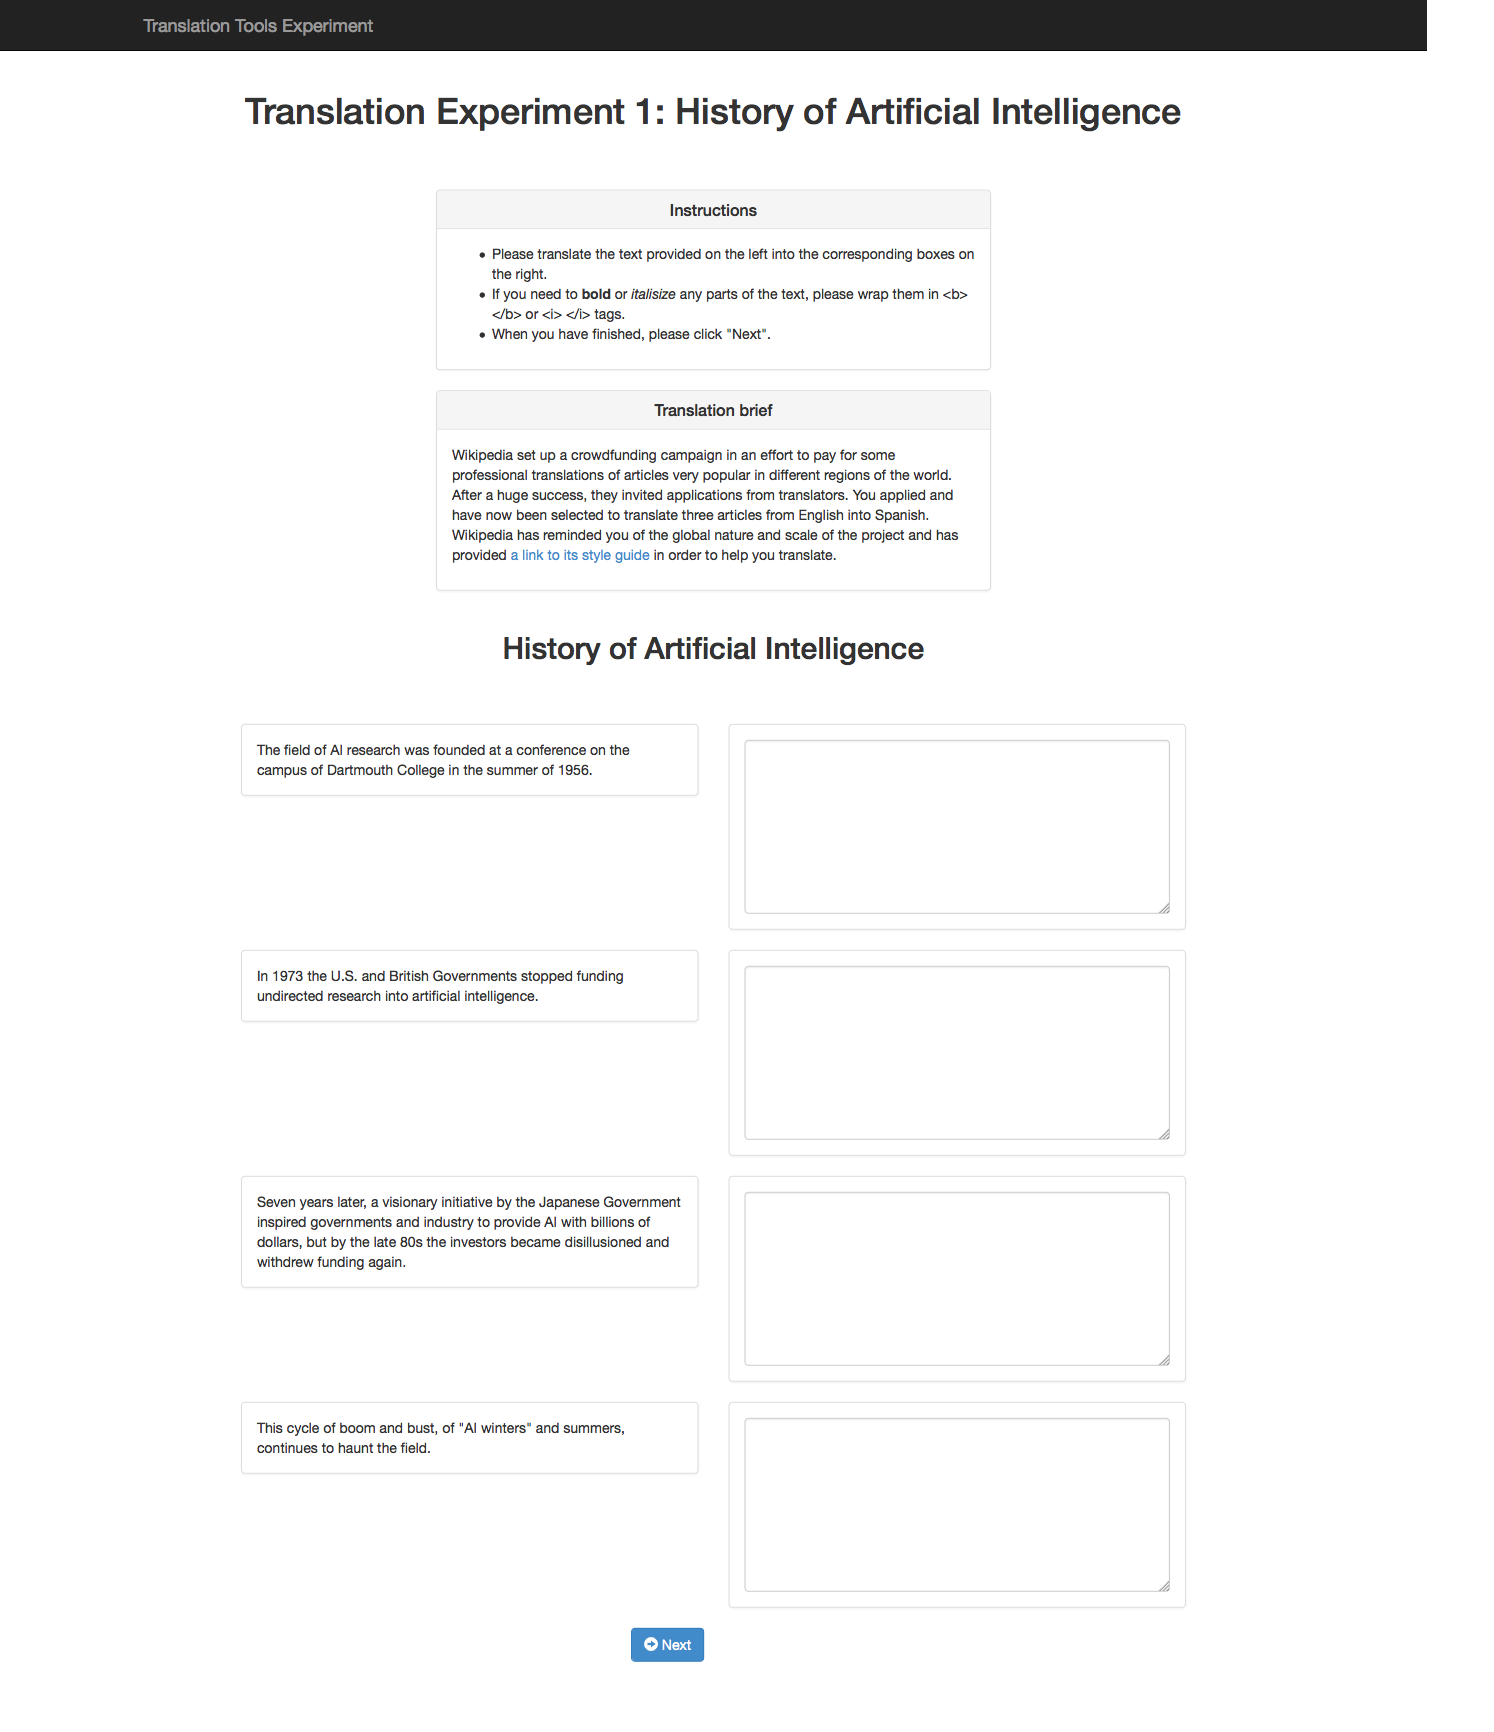
\includegraphics[width=\textwidth]{img/web/web_4.png}
\caption{Website (Page 4). Participants translate in the from-scratch setup.}
\label{fig:web_scratch}
\end{figure}

\begin{figure}[h]
\myfloatalign
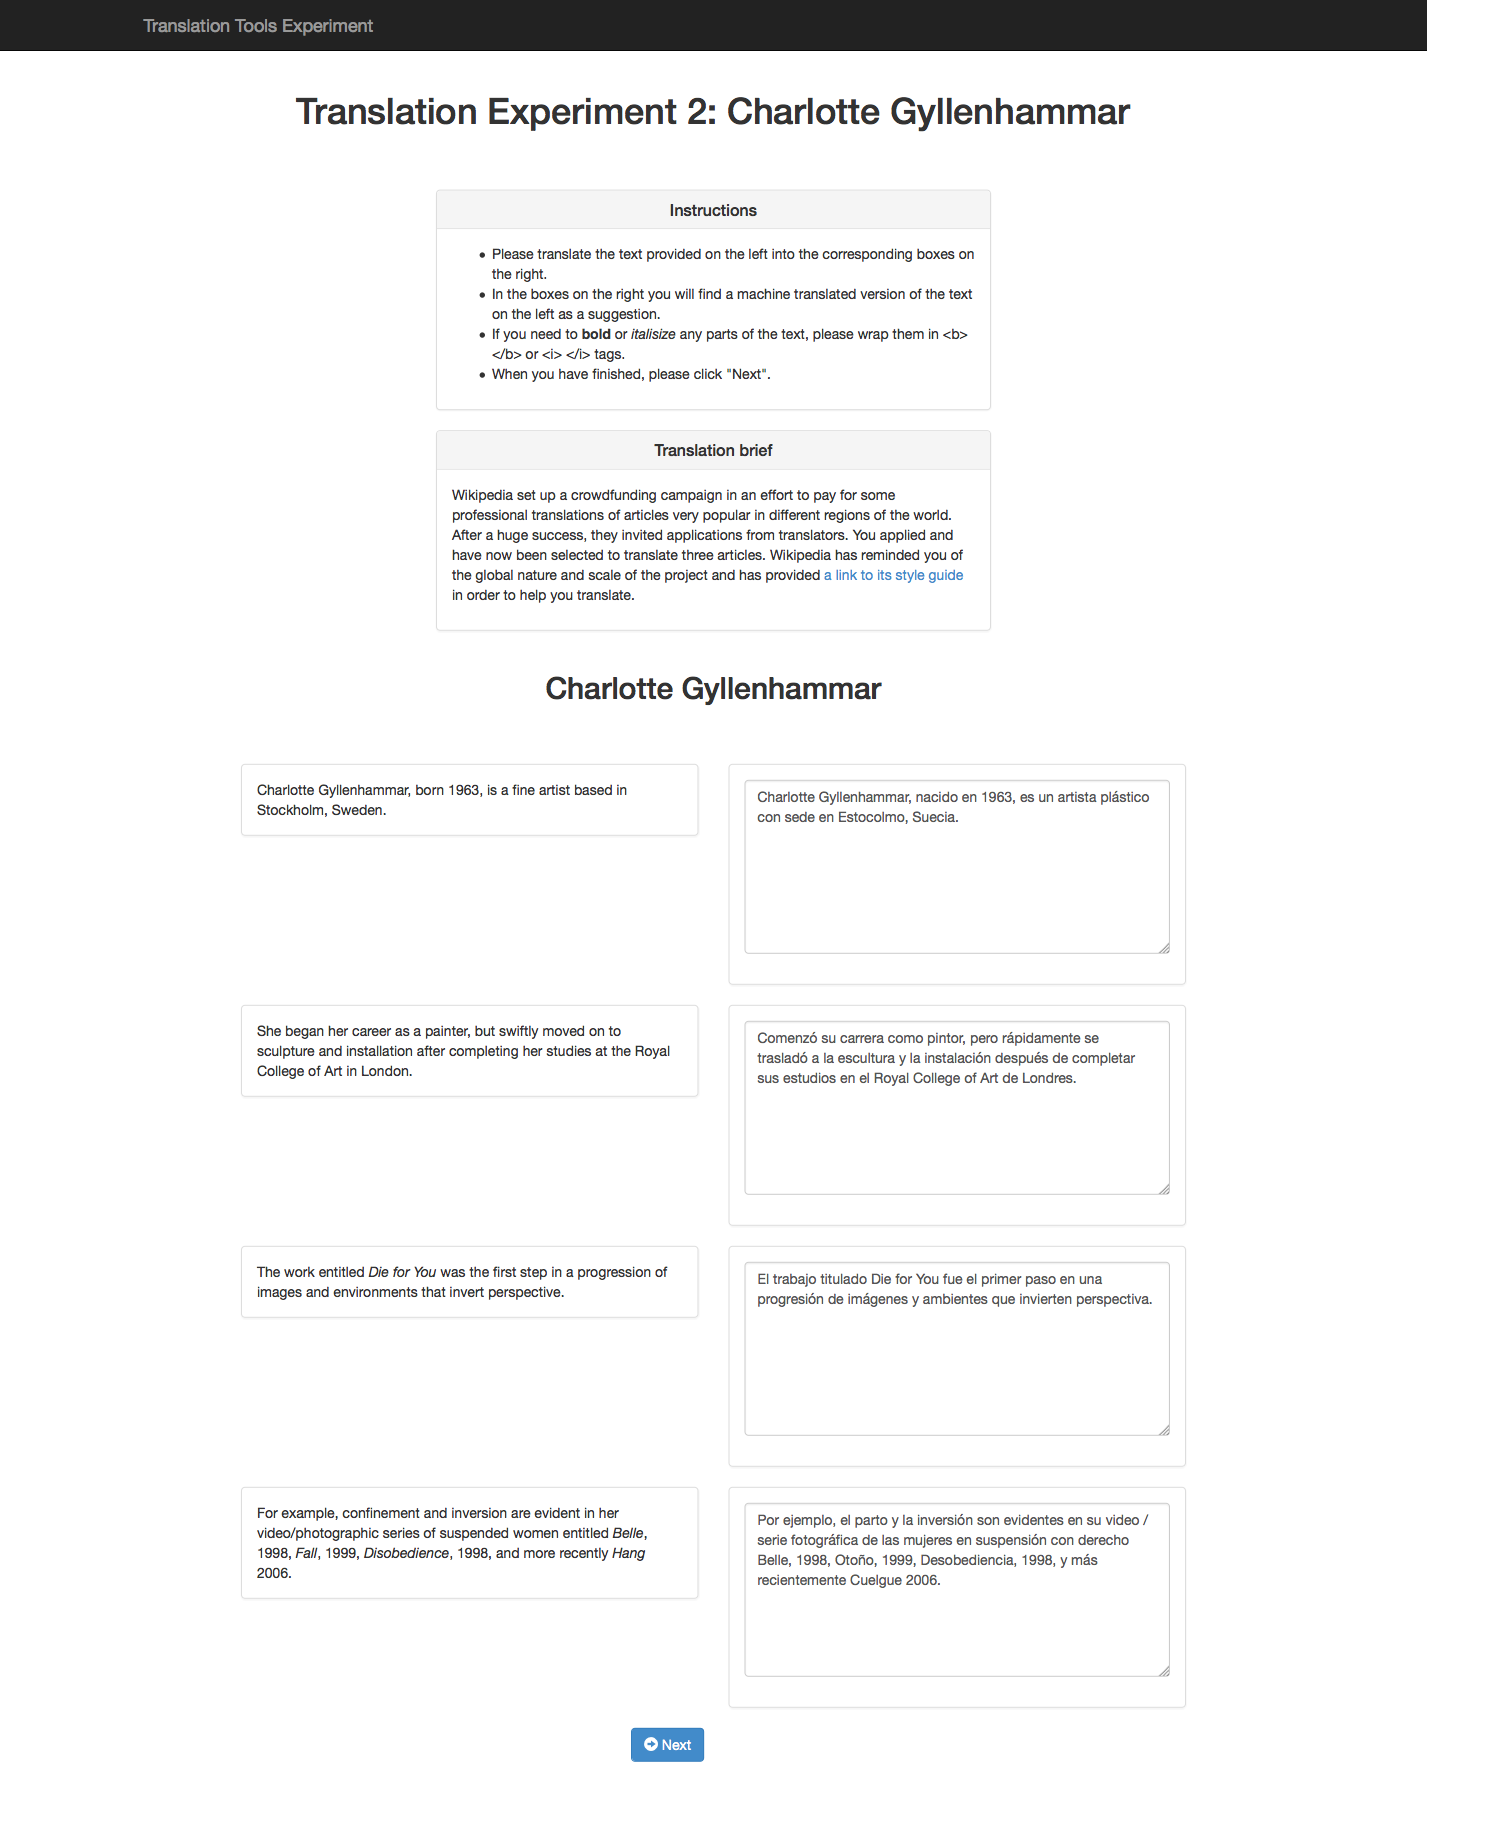
\includegraphics[width=\textwidth]{img/web/web_5.png}
\caption{Website (Page 5). Participants translate in the \ac{PE} setup.}
\label{fig:web_pe}
\end{figure}

\begin{figure}[h]
\myfloatalign
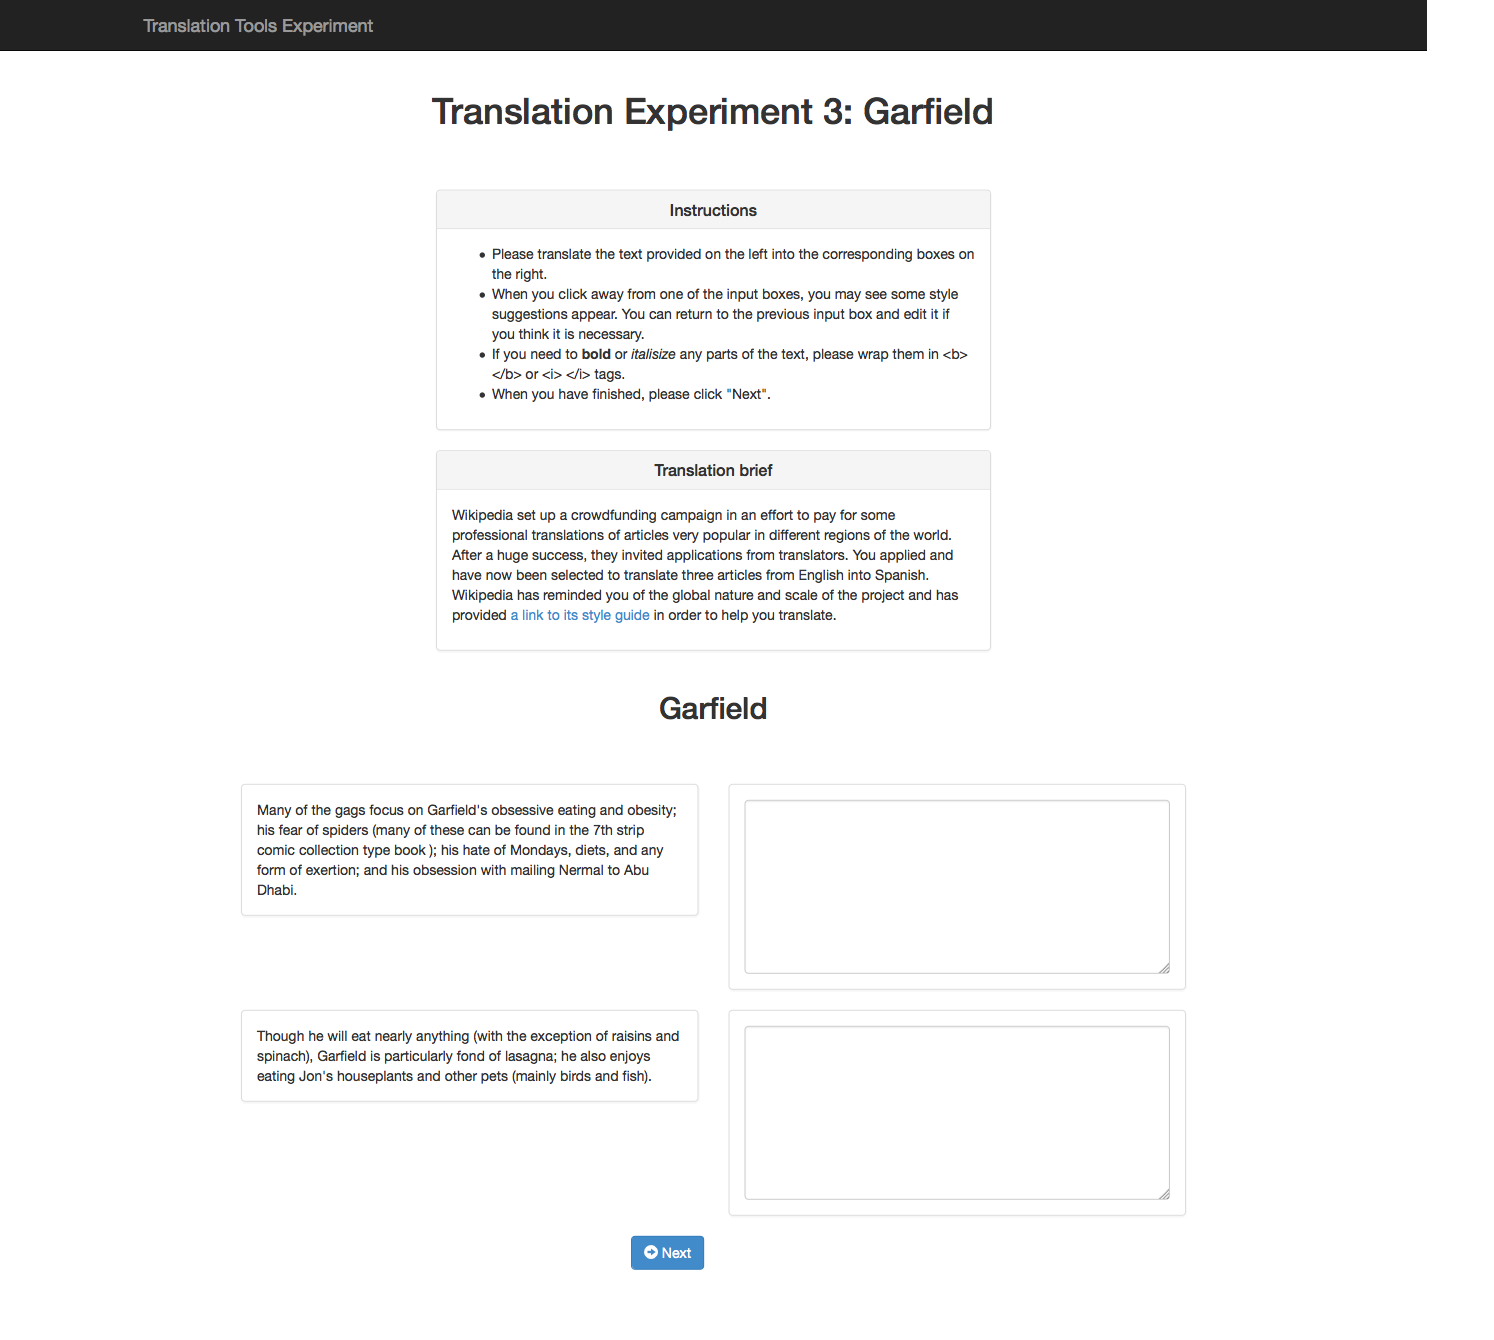
\includegraphics[width=\textwidth]{img/web/web_6.png}
\caption{Website (Page 6). Participants translate in the style setup.}
\label{fig:web_style}
\end{figure}

Finally, participants were asked to complete the final questionnaire (\autoref{fig:web_final}). They were provided with the \ac{ST} of the translations they had completed (and the \ac{MT} suggestion in the \ac{PE} setup) to help jog their memory. Finally, participants are thanked for their participation (\autoref{fig:web_thanks}).

\begin{figure}[h]
\myfloatalign
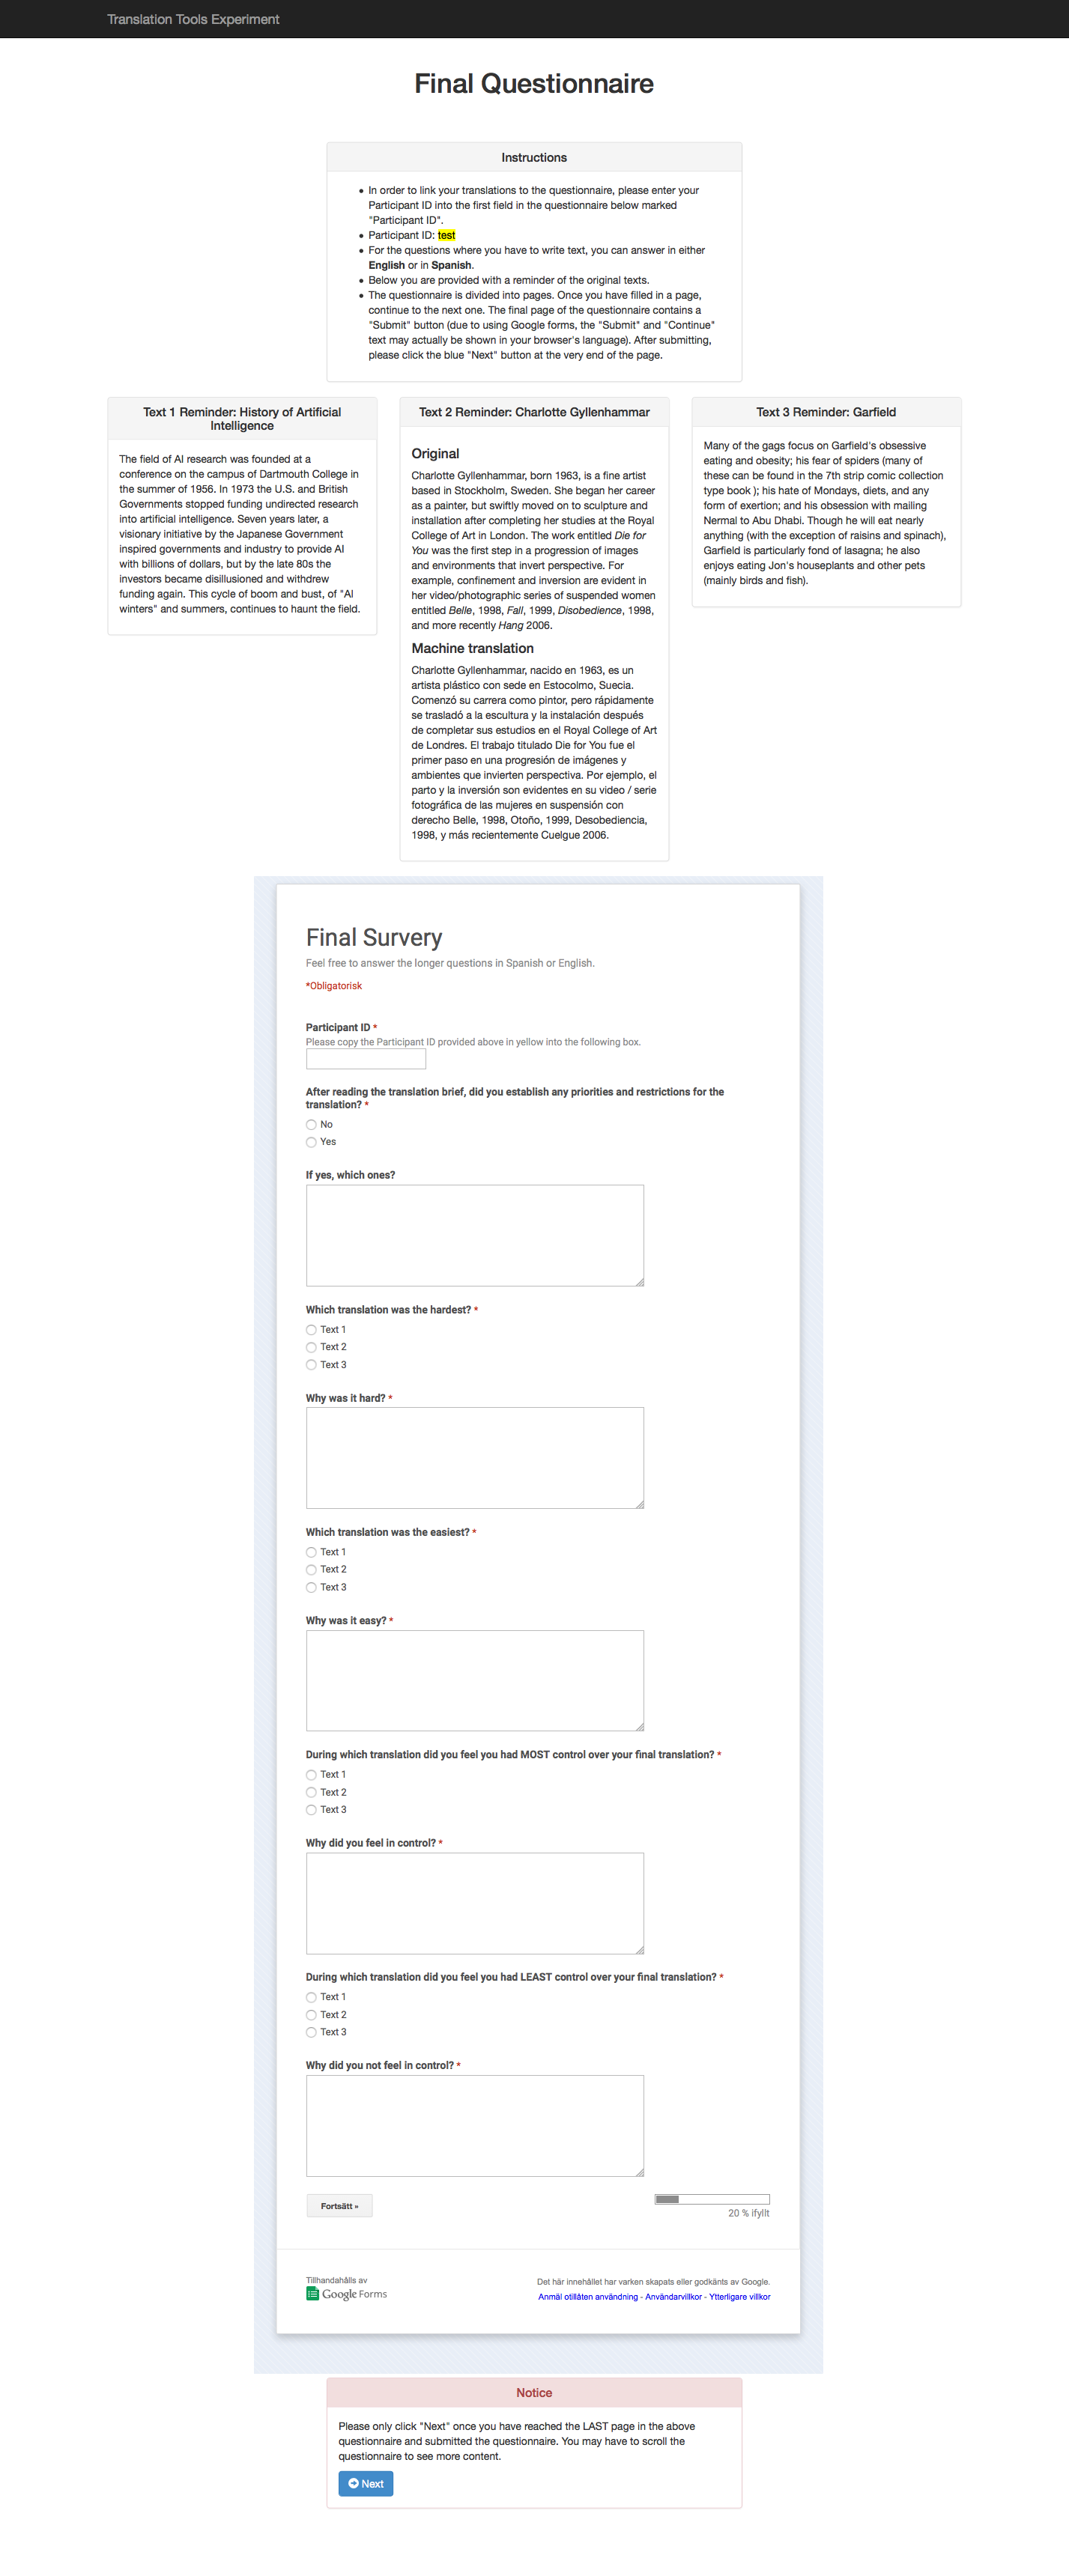
\includegraphics[height=\textheight]{img/web/web_7.png}
\caption{Website (Page 7). Participants are asked to answer the final questionnaire.}
\label{fig:web_final}
\end{figure}

\begin{figure}[h]
\myfloatalign
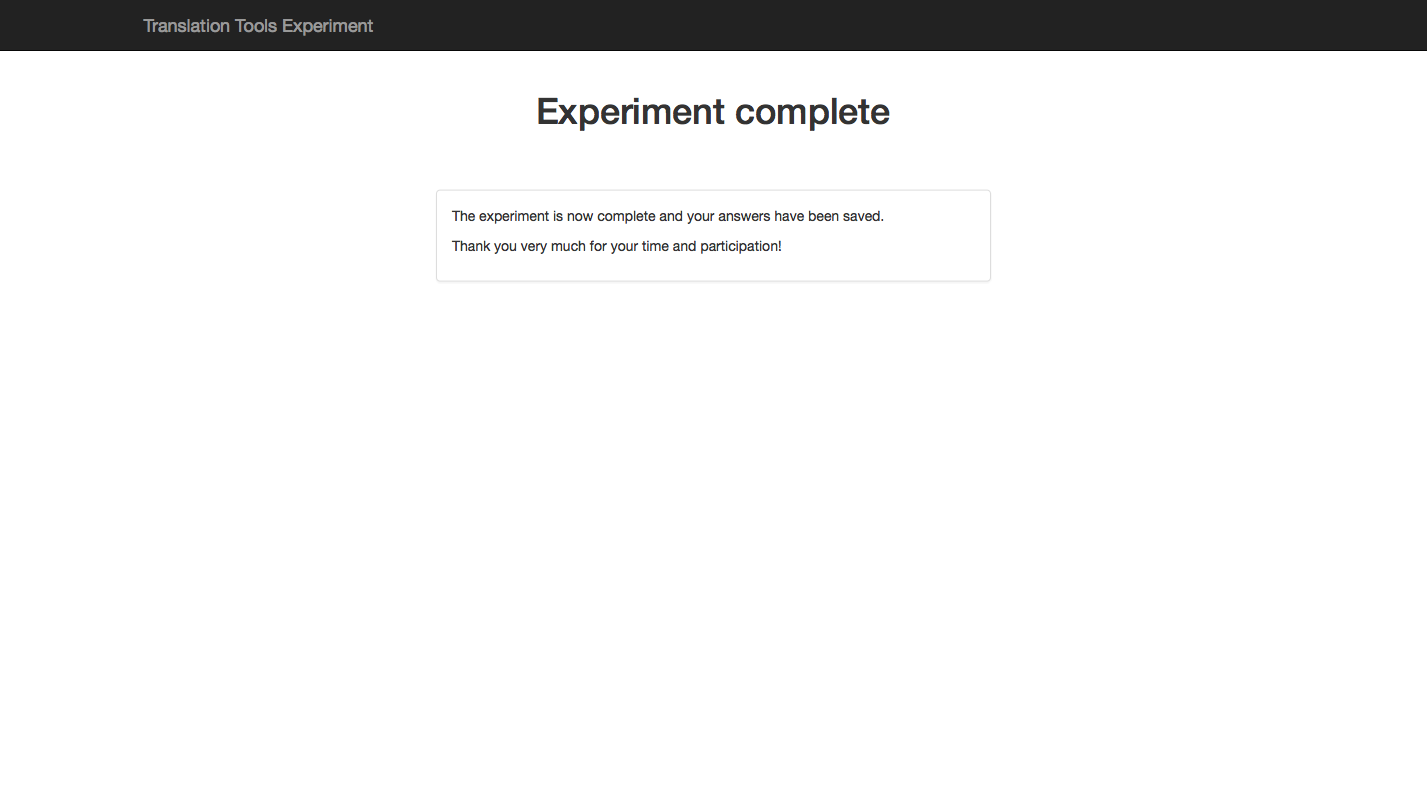
\includegraphics[width=\textwidth]{img/web/web_8.png}
\caption{Website (Page 7). Participants are thanked for their collaboration.}
\label{fig:web_thanks}
\end{figure}
 % Appendix Experiment Walkthrough
% Appendix A

\chapter{Questionnaires}
\label{an:questionnaires}

%----------------------------------------------------------------------------------------

\noindent This appendix contains screenshots of both the initial (before translating) and final (after translating) questionnaires that were given to the study's participants. For further details on the design of the questionnaires, please refer to \autoref{ch:questionnaires}.

\paragraph{Please Note:} Form navigation and interface elements, such as the ``Next'' and ``Submit'' buttons and ``Required*'' field, were shown in the language participants have their Google account set up in or, if they don't have one, in the browser's default language. The screenshots in this chapter show the navigation and interface elements in Swedish, but this varied for each participant.

%----------------------------------------------------------------------------------------

\section{Initial Questionnaire}

\subsection{Questions}

\graffito{Note: in case of closed questions, the possible options are shown in square brackets.}

\begin{enumerate}
\item What does translation mean to you? 
\item What is your gender? [Male, Female, Other]
\item What is your year of birth? 
\item What is your current occupation?
\item Which language(s) are you native in? [English, Spanish, French, German, Catalan, Basque, Galician, Chinese, Japanese, Portuguese, Italian, Russian, Greek, Other]
\item Which other language(s) do you speak? [English, Spanish, French, German, Catalan, Basque, Galician, Chinese, Japanese, Portuguese, Italian, Russian, Greek, Other]
\item Have you studied translation? [Yes, No]
\item If yes, for how many years have you studied translation?
\item Have you worked as a translator? [Yes, No]
\item If yes, for how many years have you worked as a translator?
\item Do you have professional experience working on the following translation-related tasks? [Multiple choices can be selected] [Translating from scratch, Proof-reading, Machine translation post-editing, Transcreation, Loclalizing, Managing terminology, Setting-up style guides, Translating with a CAT tool (For example, Trados), Preparing documents for internationalisation, Machine translation system setup (for example, Moses SMT), Machine translation quality evaluation]
\item What do you think are the most INTERESTING tasks to carry out when translating?
\item What do you think are the most BORING tasks to carry out when translating?
\item If a tool could be created to automate any task you carry out when translating so you don't have to do it, which task would it be?
\item How important are the following considerations when translating? [Very important (1), (2), (3), (4), Not at all important (5)]
\begin{enumerate}
\item Accurately portraying the source text
\item Applying a style guide consistently
\item Using terminology consistently
\item Providing a grammatically correct translation
\item Conforming to what the client requests in the translation brief
\item Providing a fluent translation/idiomatic translation
\end{enumerate}
\item Which of the previous considerations do you prioritise the most? [Accurately portraying the source text, Applying a style guide consistently, Using terminology consistently, Providing a grammatically correct translation, Conforming to what the client requests in the translation brief, Providing a fluent translation/idiomatic translation]
\item Are there any other considerations you usually take into account?
\item Do you usually use glossaries / terminological lists when translating? [Yes, No]
\item Do you usually use style guides when translating? [Yes, No]
\item Do you usually use computer-aided translation (CAT) when translating? [Yes, No]
\item Do you agree with the following statements? [Strongly agree (1), (2), (3), (4), Strongly Disagree (5)]
\begin{enumerate}
\item Machine translation is useful for translators
\item Machine translation is ONLY useful for the general public
\item Machine translation will one day replace human translators
\item Machine translation today provides good quality translations
\item It is difficult to understand how machine translation works
\item I would like to learn more about machine translation
\end{enumerate}
\item Do you think your translations are better than those from machine translation? [Yes, No]
\item Why?
\end{enumerate}

\subsection{Screenshots}

\noindent The following are screenshots of the questionnaire that participants had to fill in before starting the translation tasks.

\begin{figure}[H]
\myfloatalign
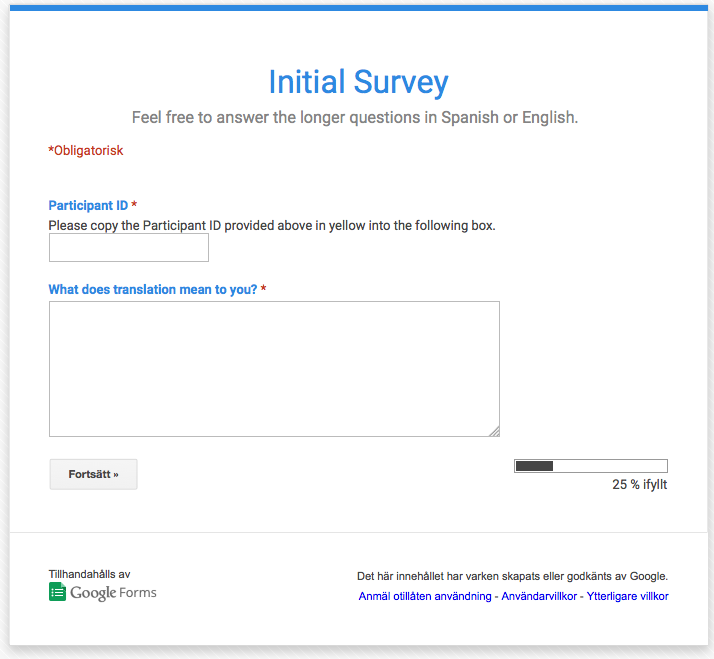
\includegraphics[width=\textwidth]{img/initial_questionnaire/initial_1.png}
\caption{Initial Questionnaire (Page 1)}
\end{figure}

\begin{figure}[H]
\myfloatalign
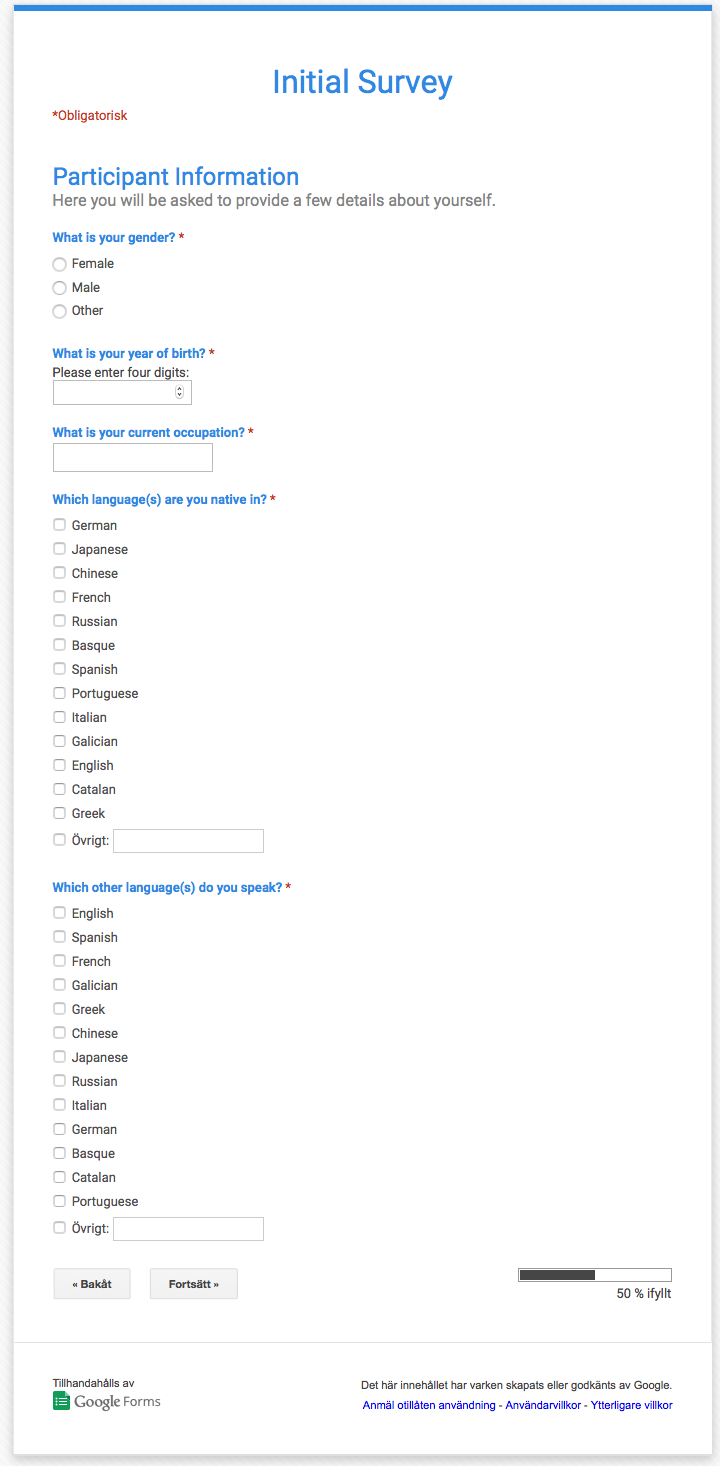
\includegraphics[height=\textheight]{img/initial_questionnaire/initial_2.png}
\caption{Initial Questionnaire (Page 2)}
\end{figure}

\begin{figure}[H]
\myfloatalign
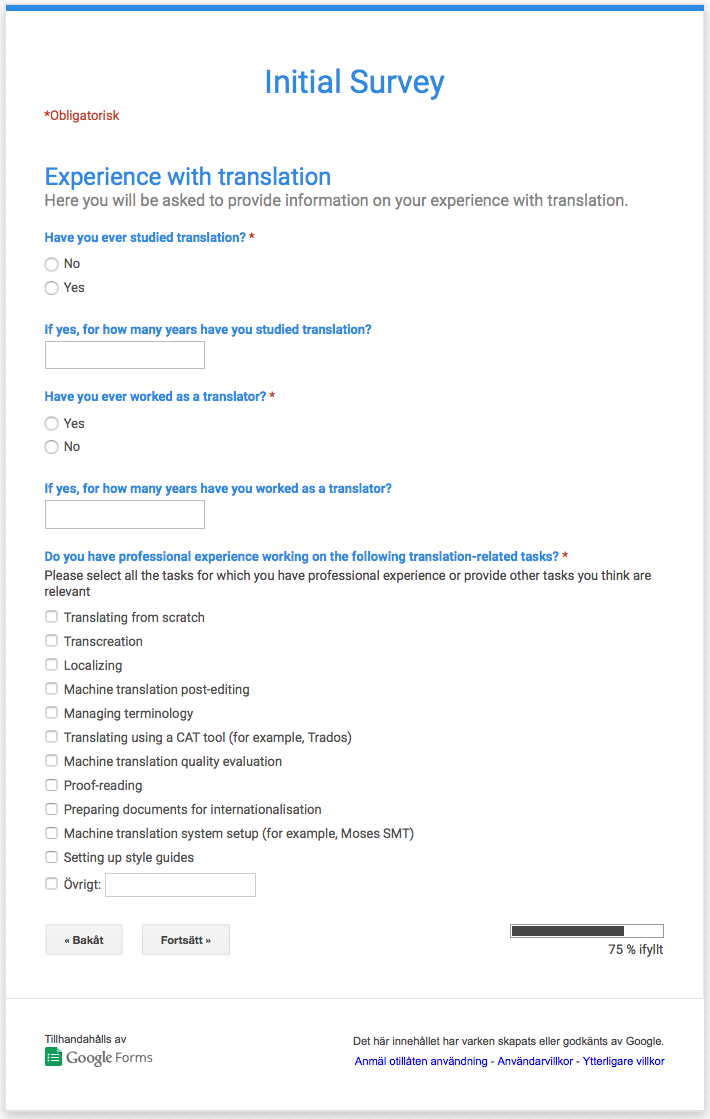
\includegraphics[width=\textwidth]{img/initial_questionnaire/initial_3.png}
\caption{Initial Questionnaire (Page 3)}
\end{figure}

\begin{figure}[H]
\myfloatalign
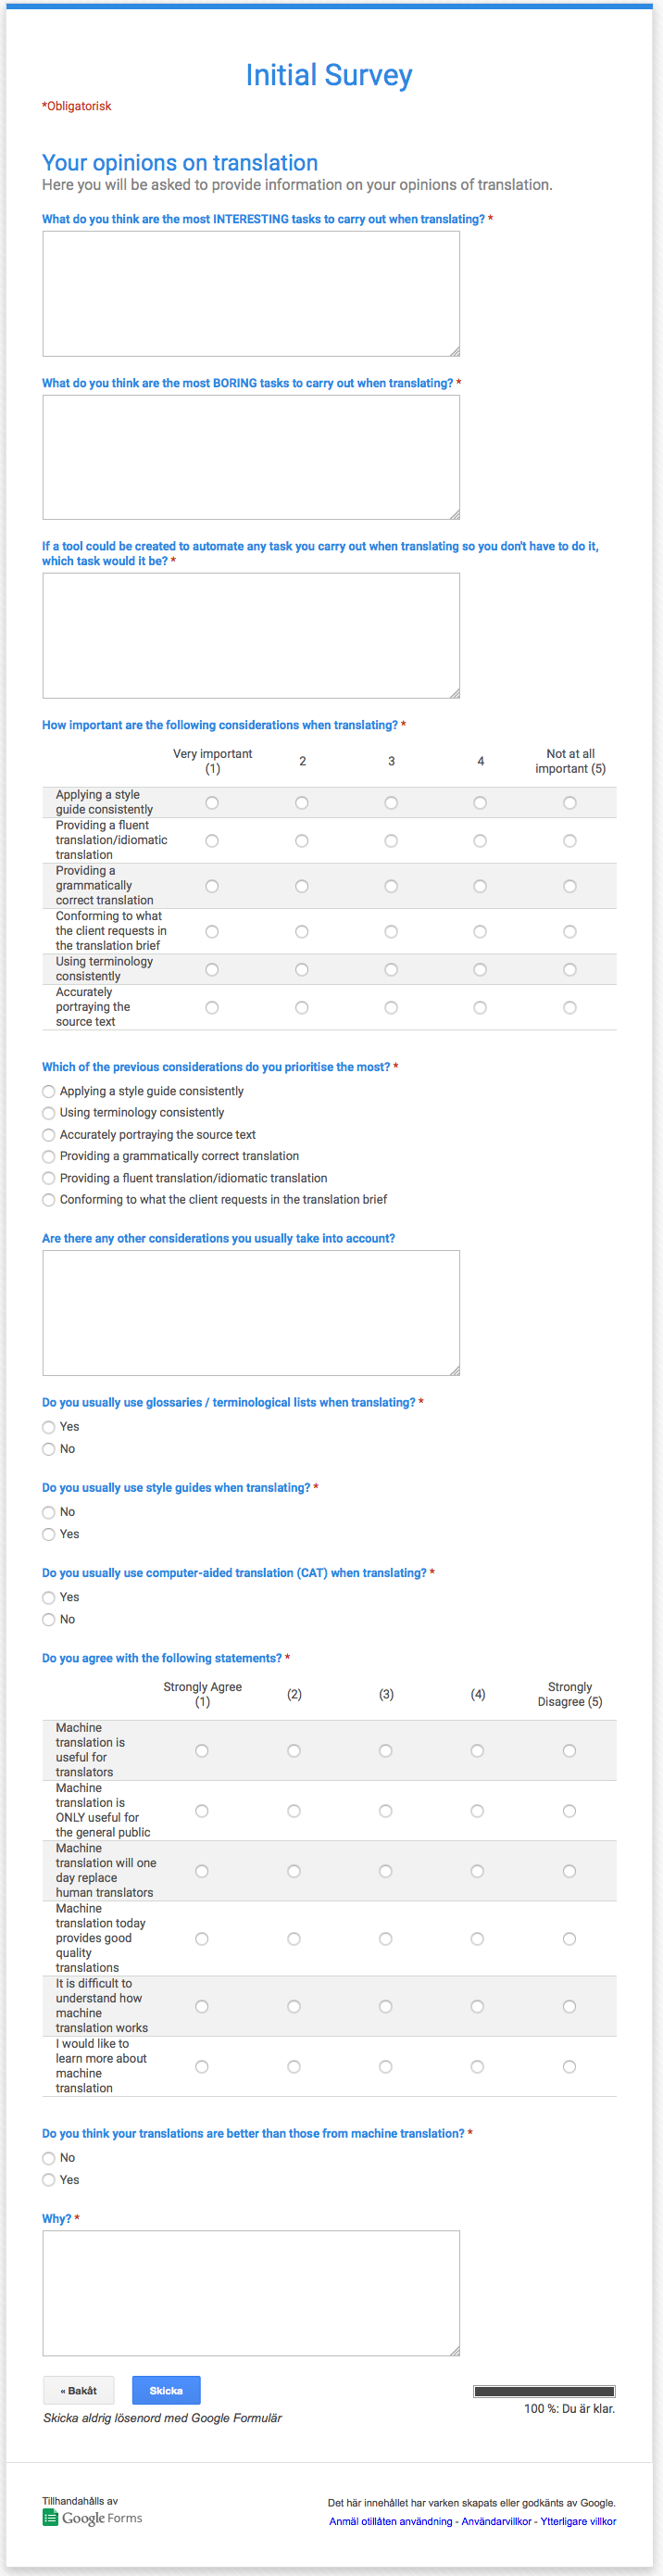
\includegraphics[height=\textheight]{img/initial_questionnaire/initial_4.png}
\caption{Initial Questionnaire (Page 3)}
\end{figure}

\newpage
%----------------------------------------------------------------------------------------

\section{Final Questionnaire}

\subsection{Questions}

\graffito{Note: in case of closed questions, the possible options are shown in square brackets.}

\begin{enumerate}
    \item After reading the translation brief, did you establish any priorities and restrictions for the translation? [Yes, No]
    \item If yes, which ones?
    \item Which translation was the hardest? [Text 1, Text 2, Text 3]
    \item Why was it hard?
    \item Which translation was the easiest? [Text 1, Text 2, Text 3]
    \item Why was it easy?
    \item During which translation did you feel you had MOST control over your final translation? [Text 1, Text 2, Text 3]
    \item Why did you feel in control?
    \item During which translation did you feel you had LEAST control over your final translation? [Text 1, Text 2, Text 3]
    \item Why did you not feel in control?
    \item Approximately, how many minutes do you think it took you to translate Text 1?
    \item What did you LIKE the most about translating Text 1?
    \item What did you DISLIKE the most about translating Text 1?
    \item Overall, how satisfied were you with the task of translating Text 1? [Very satisfied, Somewhat satisfied, Neutral, Somewhat dissatisfied, Very dissatisfied]
    \item Overall, how satisfied were you with the quality of your final translation of Text 1? [Very satisfied, Somewhat satisfied, Neutral, Somewhat dissatisfied, Very dissatisfied]
    \item Do you have any additional comments on the translation of Text 1?
    \item Approximately, how many minutes do you think it took you to translate Text 2?
    \item What did you LIKE the most about translating Text 2?
    \item What did you DISLIKE the most about translating Text 2?
    \item How would you rate the quality of the machine translation suggestions? [Well below average, Below average, Average, Above average, Well above average]
        \begin{enumerate}
            \item Grammaticality
            \item Style
            \item Accuracy
        \end{enumerate}
    \item Would you have preferred to translate from scratch without the machine translation suggestions? [Yes, No]
    \item Overall, how satisfied were you with the task of translating Text 2? [Very satisfied, Somewhat satisfied, Neutral, Somewhat dissatisfied, Very dissatisfied]
    \item Overall, how satisfied were you with the quality of your final translation of Text 2? [Very satisfied, Somewhat satisfied, Neutral, Somewhat dissatisfied, Very dissatisfied]
    \item Do you have any additional comments on the translation of Text 2?
    \item Approximately, how many minutes do you think it took you to translate Text 3?
    \item What did you LIKE the most about translating Text 3?
    \item What did you DISLIKE the most about translating Text 3?
    \item Did you consult the Wikipedia Style Guide linked to in the Translation Brief? [Yes, No]
    \item Why?
    \item Do you agree with the following statements? [Strongly agree (1), (2), (3), (4), Strongly Disagree (5)]
        \begin{enumerate}
            \item The style hints were helpful
            \item There were too many style hints
            \item The style hints were easy to understand
            \item The style hints were too long
            \item The boxes where the style hints were shown were distracting
            \item The style hints contained wrong information
        \end{enumerate}
    \item Would you have preferred to translate from scratch without the style suggestions? [Yes, No]
    \item Overall, how satisfied were you with the task of translating Text 3? [Very satisfied, Somewhat satisfied, Neutral, Somewhat dissatisfied, Very dissatisfied]
    \item Overall, how satisfied were you with the quality of your final translation of Text 3? [Very satisfied, Somewhat satisfied, Neutral, Somewhat dissatisfied, Very dissatisfied]
    \item Do you have any additional comments on the translation of Text 3?
    \item Do you have any final comments about any aspect of the experiment?
\end{enumerate}

\subsection{Screenshots}

\noindent The following are screenshots of the questionnaire that participants had to fill in after completing the translation tasks. Participants were shown a reminder (not seen in the following screeenshots) of the source texts they had translated to help job their memory.

\begin{figure}[h]
\myfloatalign
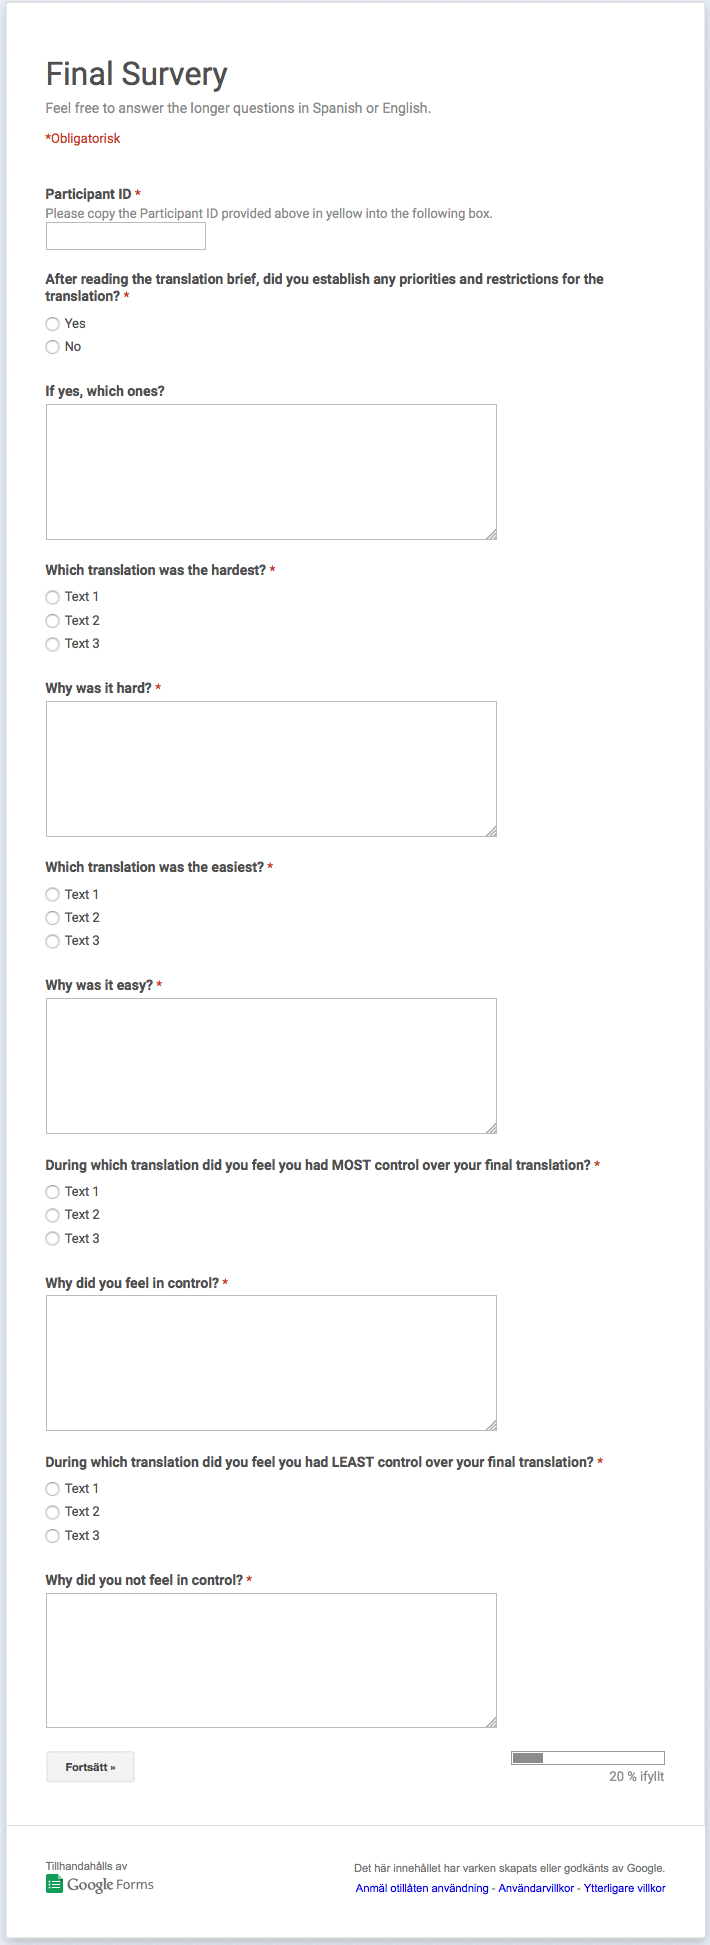
\includegraphics[height=\textheight]{img/final_questionnaire/final_1.png}
\caption{Final Questionnaire (Page 1)}
\end{figure}

\begin{figure}[h]
\myfloatalign
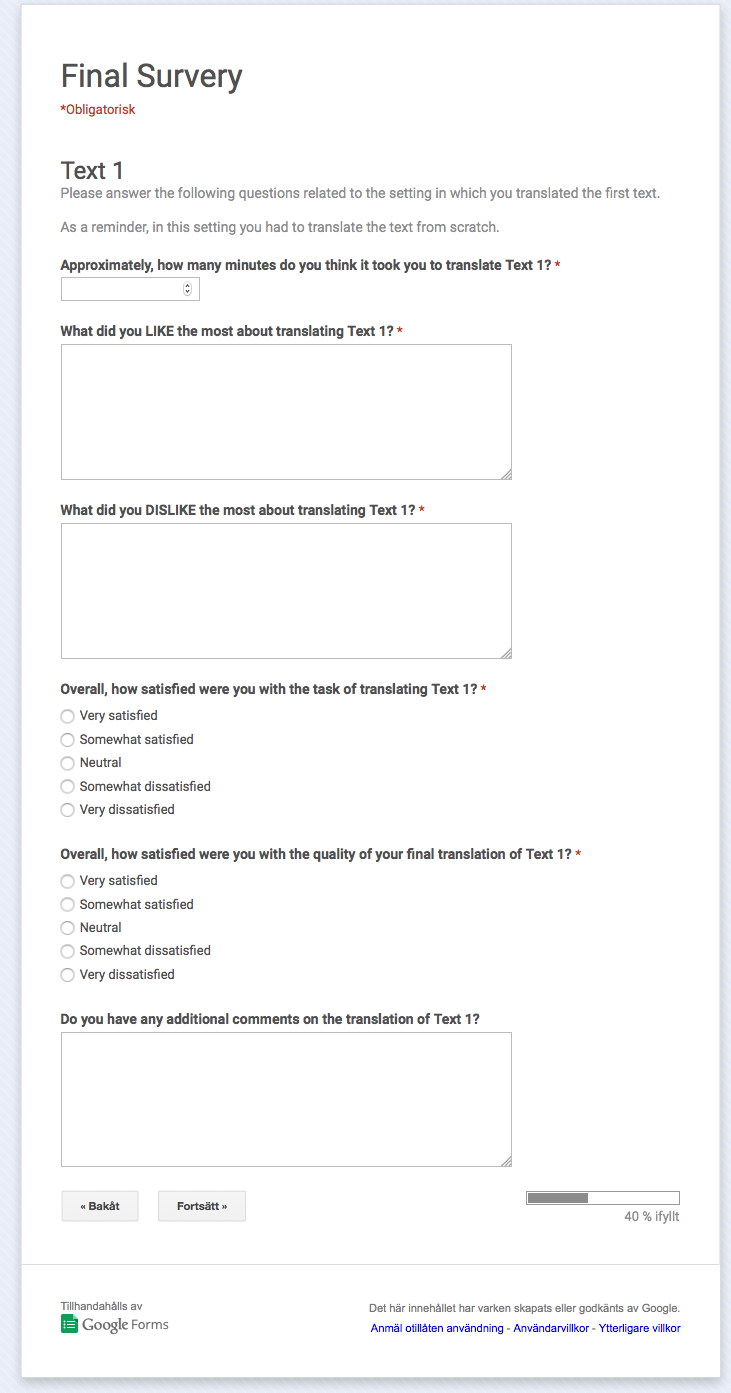
\includegraphics[height=\textheight]{img/final_questionnaire/final_2.png}
\caption{Final Questionnaire (Page 2)}
\end{figure}

\begin{figure}[h]
\myfloatalign
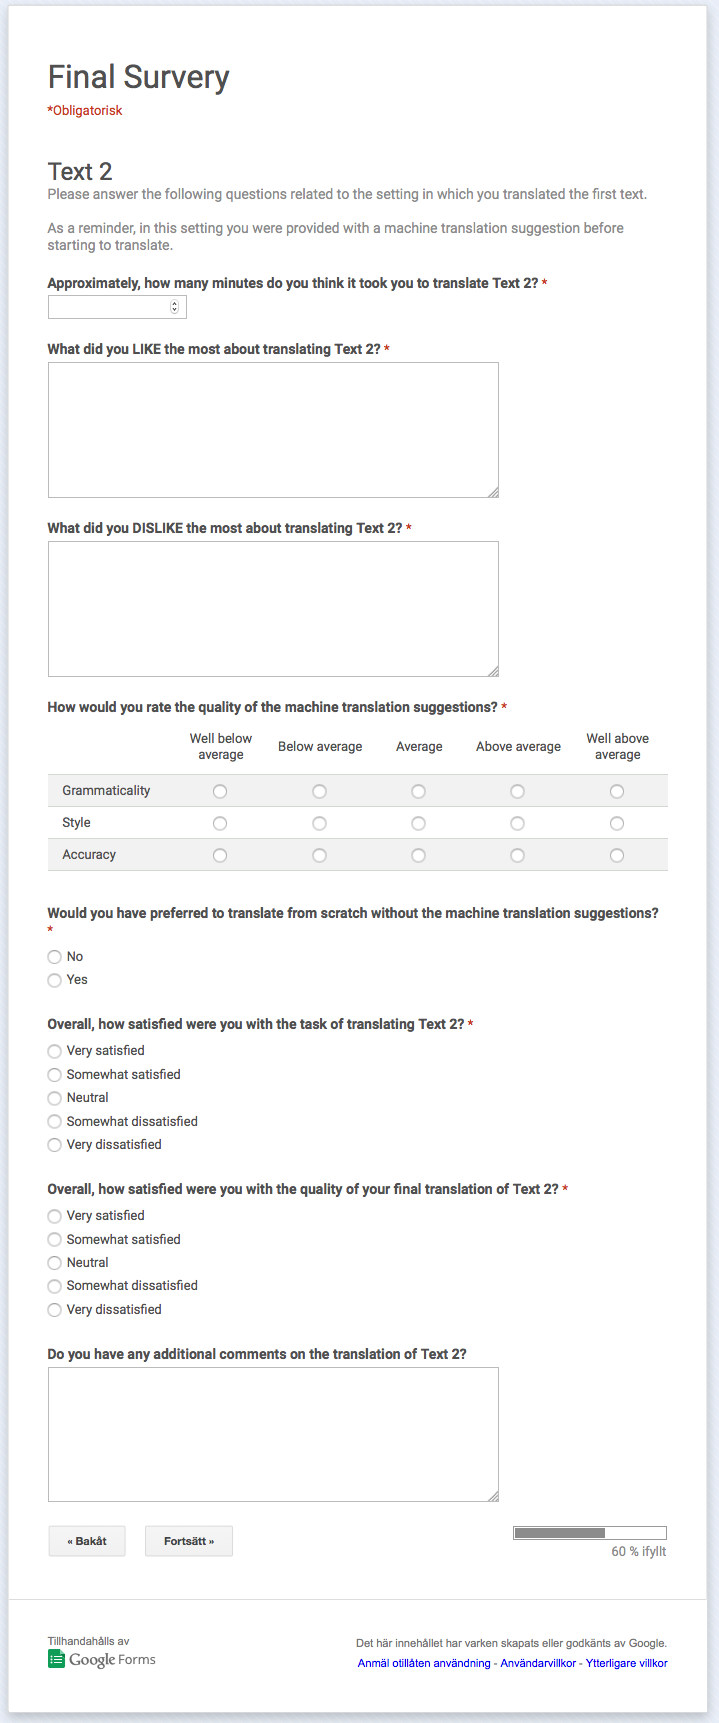
\includegraphics[height=\textheight]{img/final_questionnaire/final_3.png}
\caption{Final Questionnaire (Page 3)}
\end{figure}

\begin{figure}[h]
\myfloatalign
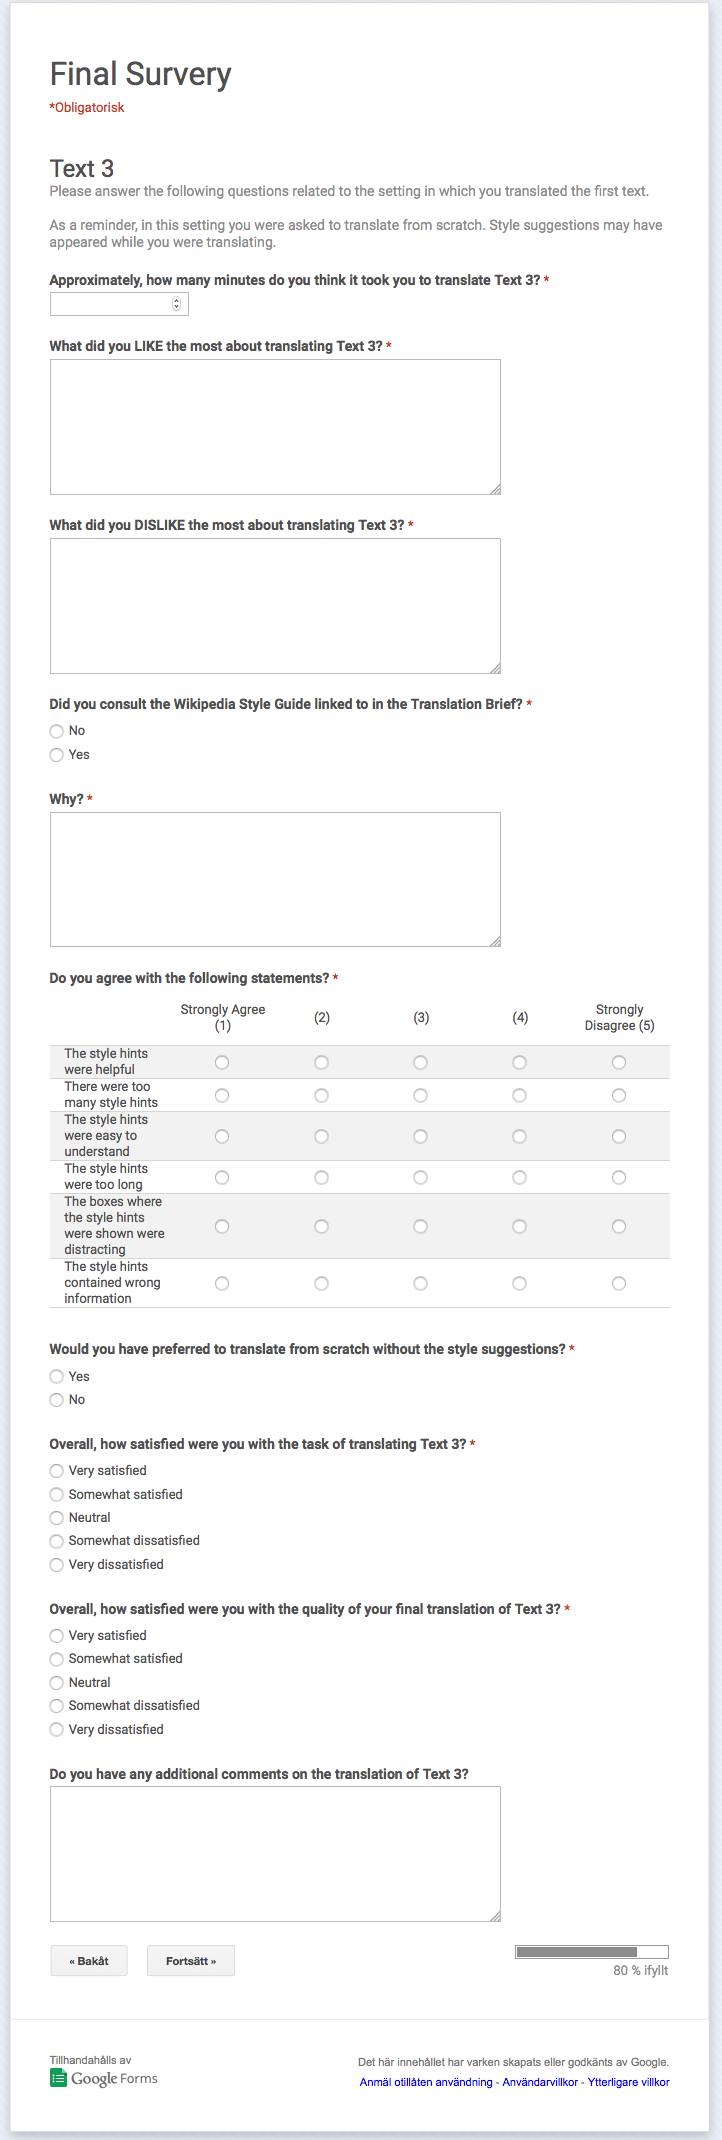
\includegraphics[height=\textheight]{img/final_questionnaire/final_4.png}
\caption{Final Questionnaire (Page 4)}
\end{figure}

\begin{figure}[h]
\myfloatalign
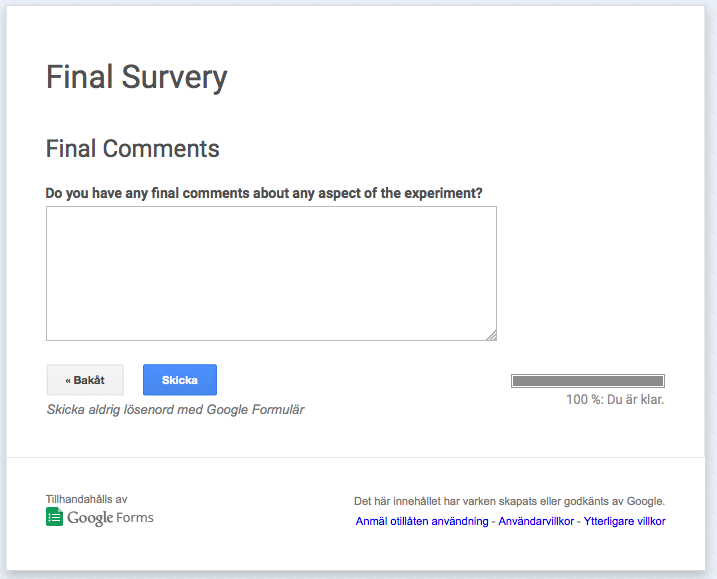
\includegraphics[width=\textwidth]{img/final_questionnaire/final_5.png}
\caption{Final Questionnaire (Page 5)}
\end{figure}
 % Appendix Questionnaires
% Appendix X

\chapter{Wikipedia Texts}
\label{app:texts}

%----------------------------------------------------------------------------------------

% Content begins here

\section{Source Texts}

\noindent The following subsections contain the Wikipedia texts that participants were asked to translate. All links to other Wikipedia articles were removed and not shown to participants, as it was considered too much work for this experiment to ensure that the translation contained the correct links in Spanish.

\subsection{History of Artificial Intelligence}

\begin{quotation}
\noindent The field of AI research was founded at a conference on the campus of Dartmouth College in the summer of 1956. 

[\dots]

In 1973 [\dots] the U.S. and British Governments stopped funding undirected research into artificial intelligence. Seven years later, a visionary initiative by the Japanese Government inspired governments and industry to provide AI with billions of dollars, but by the late 80s the investors became disillusioned and withdrew funding again. This cycle of boom and bust, of "AI winters" and summers, continues to haunt the field.
\flushright\parencite{wikihistory}
\end{quotation}

\subsection{Charlotte Gyllenhammer}

\noindent A slight motification was introduced to this text in order to include a style error. The Wikipedia Spanish Style Guide \parencite{wikistyle} states that lists which can be ordered chronologically, should be ordered in this fashion. Although the original text correctly ordered the artist's works (``\textit{Belle}, 1998, \textit{Disobedience}, 1998, \textit{Fall}, 1999, and more recently \textit{Hang} 2006''), the order of \textit{Disobedience} and \textit{Fall} was swapped, making a clearly unordered list. Also, the bold font styling of ``\textbf{Charlotte Gyllenhammer}'' was removed as it was deemed there were sufficient other style guide considerations in the text.

\begin{quotation}
\noindent Charlotte Gyllenhammar, born 1963, is a fine artist based in Stockholm, Sweden. She began her career as a painter, but swiftly moved on to sculpture and installation after completing her studies at the Royal College of Art in London. 

[\dots] 

The work entitled \textit{Die for You} was the first step in a progression of images and environments that invert perspective. For example, confinement and inversion are evident in her video/photographic series of suspended women entitled \textit{Belle}, 1998, \textit{Fall}, 1999,\textit{Disobedience}, 1998, and more recently \textit{Hang} 2006.
\flushright\parencite{wikicharlotte}
\end{quotation}

\subsection{Garfield}

\noindent The first sentence of the text was shortened from the original, since the long length of the paragraph slowed down the StyleCheck tool and could even block it. The original read ``[\dots] any form of exertion; his constant shedding (which constantly annoys Jon); and his abuse of Odie and Jon as well as his obsession with mailing Nermal to Abu Dhabi.''


\begin{quotation}
\noindent Many of the gags focus on Garfield's obsessive eating and obesity; his fear of spiders (many of these can be found in the 7th strip comic collection type book ); his hate of Mondays, diets, and any form of exertion; and his obsession with mailing Nermal to Abu Dhabi.  Though he will eat nearly anything (with the exception of raisins and spinach), Garfield is particularly fond of lasagna; he also enjoys eating Jon's houseplants and other pets (mainly birds and fish).
\flushright\parencite{wikigarfield}
\end{quotation}

\section{MT Translation Suggestions}

\noindent Machine translation suggestions were obtained by running the text fragments through Google Translate\footnote{\url{https://translate.google.com/}, translations were carried out on 4 May 2015.}. Below are the results as they were used in the \ac{PE} setup of the experiments.

\subsection{History of Artificial Intelligence (MT)}

\begin{quotation}
\noindent El campo de la investigación en IA fue fundada en una conferencia en el campus de la universidad de Dartmouth en el verano de 1956.

En 1973 los EE.UU. y los gobiernos británicos detuvimos financiación de la investigación no dirigida en inteligencia artificial. Siete años más tarde, una iniciativa visionaria de los gobiernos Gobierno inspirado japonés y la industria para proporcionar AI con miles de millones de dólares, pero a finales de los años 80 los inversores se desilusionó y se retiró la financiación de nuevo. Este ciclo de auge y caída, de los "inviernos y veranos AI", sigue acosando el campo.
\end{quotation}

\subsection{Charlotte Gyllenhammer (MT)}

\begin{quotation}
\noindent Charlotte Gyllenhammar, nacido en 1963, es un artista plástico con sede en Estocolmo, Suecia. Comenzó su carrera como pintor, pero rápidamente se trasladó a la escultura y la instalación después de completar sus estudios en el Royal College of Art de Londres.

El trabajo titulado Die for You fue el primer paso en una progresión de imágenes y ambientes que invierten perspectiva. Por ejemplo, el parto y la inversión son evidentes en su video / serie fotográfica de las mujeres en suspensión con derecho Belle, 1998, Otoño, 1999, Desobediencia, 1998, y más recientemente Cuelgue 2006.
\end{quotation}

\subsection{Garfield (MT)}

\begin{quotation}
\noindent Muchos de los gags se centran en la alimentación y la obesidad obsesivo de Garfield; su miedo a las arañas (muchos de ellos se puede encontrar en el séptimo tira tipo de colección cómica del libro); su odio de los lunes, dietas, y cualquier forma de ejercicio; y su obsesión por correo Nermal a Abu Dhabi. A pesar de que va a comer casi cualquier cosa (con la excepción de las pasas y las espinacas), Garfield es particularmente aficionado a la lasaña; también le gusta comer las plantas de interior de Jon y otros animales (principalmente aves y peces).
\end{quotation}

 % Appendix Texts
% Appendix X

\chapter{StyleCheck Grammar}
\label{app:code}

%----------------------------------------------------------------------------------------

\section{Wiki Abstract Syntax}

\lstinputlisting[caption={Abstract syntax where the style rules are defined}, label=lst:wiki]{Code/Wiki.gf}

\section{WikiMaster Concrete Syntax}

\lstinputlisting[caption={Main concrete syntax where the style records are built}, label=lst:wikimaster]{Code/WikiMaster.gf}

\section{WikiHint Concrete Syntax}

\lstinputlisting[caption={Concrete syntax where the hints are selected from the style records}, label=lst:wikihint]{Code/WikiHint.gf}

 % Appendix Code


%----------------------------------------------------------------------------------------
%	POST-CONTENT THESIS PAGES
%----------------------------------------------------------------------------------------

\cleardoublepage% Bibliography

\label{app:bibliography} 

\manualmark
\markboth{\spacedlowsmallcaps{\bibname}}{\spacedlowsmallcaps{\bibname}} 
\refstepcounter{dummy}

\addtocontents{toc}{\protect\vspace{\beforebibskip}} % Place the bibliography slightly below the rest of the document content in the table of contents
\addcontentsline{toc}{chapter}{\tocEntry{\bibname}}

%\bibliographystyle{plainnat}
%\bibliography{Bibliography}

\printbibliography
 % Bibliography
\cleardoublepage
%----------------------------------------------------------------------------------------
%	List of Figures
%----------------------------------------------------------------------------------------

\manualmark
\markboth{\spacedlowsmallcaps{\listfigurename}}{\spacedlowsmallcaps{\listfigurename}} 

\refstepcounter{dummy}
\addcontentsline{toc}{chapter}{\tocEntry{\listfigurename}} % Uncomment if you would like the list of figures to appear in the table of contents
\pdfbookmark[1]{\listfigurename}{lof} % Bookmark name visible in a PDF viewer

\listoffigures

\vspace*{8ex}
\newpage

%----------------------------------------------------------------------------------------
%	List of Tables
%----------------------------------------------------------------------------------------

\refstepcounter{dummy}
\addcontentsline{toc}{chapter}{\tocEntry{\listtablename}} % Uncomment if you would like the list of tables to appear in the table of contents
\pdfbookmark[1]{\listtablename}{lot} % Bookmark name visible in a PDF viewer

\listoftables
        
\vspace*{8ex}
\newpage

    
%----------------------------------------------------------------------------------------
%	List of Listings
%---------------------------------------------------------------------------------------- 

\refstepcounter{dummy}
\addcontentsline{toc}{chapter}{\tocEntry{\lstlistlistingname}} % Uncomment if you would like the list of listings to appear in the table of contents
\pdfbookmark[1]{\lstlistlistingname}{lol} % Bookmark name visible in a PDF viewer

\lstlistoflistings 

\vspace*{8ex}
\newpage

 % Lists of tables and figures
\cleardoublepage% Colophon (a brief description of publication or production notes relevant to the edition)

\pagestyle{empty}

\hfill

\vfill

\pdfbookmark[0]{Colophon}{colophon}

\section*{Colophon}

This document was typeset using the typographical look-and-feel \texttt{classicthesis} developed by Andr\'e Miede. The style was inspired by Robert Bringhurst's seminal book on typography ``\emph{The Elements of Typographic Style}''. 
 
\bigskip

\noindent\finalVersionString
 % Colophon
%\cleardoublepage% Declaration

\refstepcounter{dummy}
\pdfbookmark[0]{Declaration}{declaration} % Bookmark name visible in a PDF viewer

\chapter*{Declaration} % Declaration section text

\thispagestyle{empty}

Put your declaration here.
\bigskip
 
\noindent\textit{\myLocation, \myTime}

\smallskip

\begin{flushright}
\begin{tabular}{m{5cm}}
\\ \hline
\centering\myName, \today \\
\end{tabular}
\end{flushright}
 % Declaration

%----------------------------------------------------------------------------------------

\end{document}
